%%% main.tex — Главный файл дипломной работы
\documentclass[a4paper,14pt]{extarticle}

%% Кодировка и язык
\usepackage[utf8]{inputenc}
\usepackage[T2A]{fontenc}
\usepackage[english,russian]{babel}

%% Шрифт Times New Roman
\usepackage{tempora}
\usepackage[scaled=0.85]{beramono}

%% Геометрия страницы (по СТО)
\usepackage[
  left=30mm,
  right=10mm,
  top=20mm,
  bottom=20mm
]{geometry}

%% Полуторный интервал
\usepackage{setspace}
\onehalfspacing

%% Абзацный отступ
\usepackage{indentfirst}
\setlength{\parindent}{1.25cm}

%% Нумерация страниц — сквозная, по центру снизу
\usepackage{fancyhdr}
\pagestyle{fancy}
\fancyhf{}
\fancyfoot[C]{\thepage}
\renewcommand{\headrulewidth}{0pt}
\renewcommand{\footrulewidth}{0pt}

%% Заголовки разделов
\usepackage{titlesec}
\titleformat{\section}
  {\normalfont\bfseries\large\centering}
  {\thesection}{1em}{}
\titleformat{\subsection}
  {\normalfont\bfseries\normalsize}
  {\thesubsection}{1em}{}
\titleformat{\subsubsection}
  {\normalfont\bfseries\normalsize}
  {\thesubsubsection}{1em}{}

%% Отступы заголовков
\titlespacing*{\section}{0pt}{2em}{1em}
\titlespacing*{\subsection}{\parindent}{1.5em}{0.5em}
\titlespacing*{\subsubsection}{\parindent}{1em}{0.5em}

%% Графика
\usepackage{graphicx}
\graphicspath{{images/}}

%% Таблицы
\usepackage{array}
\usepackage{longtable}
\usepackage{booktabs}
\usepackage{multirow}
\usepackage{tabularx}

%% Подписи к рисункам и таблицам
\usepackage[
  labelsep=endash,
  justification=centering,
  font=small
]{caption}
\DeclareCaptionLabelFormat{gost}{#1~#2}
\captionsetup{labelformat=gost}
\captionsetup[table]{justification=raggedright, singlelinecheck=false}
%% Листинги кода
\usepackage{listings}
\usepackage{xcolor}
\usepackage{fancyvrb}
\lstset{
  language=Python,
  basicstyle=\small\ttfamily,
  keywordstyle=\color{blue}\bfseries,
  commentstyle=\color{gray}\itshape,
  stringstyle=\color{red!70!black},
  numbers=left,
  numberstyle=\tiny\color{gray},
  stepnumber=1,
  numbersep=8pt,
  backgroundcolor=\color{gray!5},
  frame=single,
  rulecolor=\color{gray!30},
  breaklines=true,
  breakatwhitespace=false,
  tabsize=4,
  showstringspaces=false,
  extendedchars=true,
  inputencoding=utf8,
  captionpos=b
}

%% Стиль листинга для приложений (Courier New 11pt, интервал 1.15)
\lstdefinestyle{appendixcode}{
  language=Python,
  basicstyle=\fontsize{11}{12.65}\selectfont\fontfamily{pcr}\selectfont,
  keywordstyle=\bfseries,
  commentstyle=\itshape,
  stringstyle={},
  numbers=none,
  backgroundcolor=\color{white},
  frame=none,
  breaklines=true,
  breakatwhitespace=false,
  tabsize=4,
  showstringspaces=false,
  extendedchars=true,
  inputencoding=utf8,
  xleftmargin=0pt,
  aboveskip=0pt,
  belowskip=0pt,
}

%% Формулы
\usepackage{amsmath}
\usepackage{amssymb}

%% Гиперссылки
\usepackage[
  colorlinks=true,
  linkcolor=black,
  citecolor=black,
  urlcolor=blue
]{hyperref}

%% Приложения
\usepackage[title]{appendix}

%% Содержание — точки между названием и номером страницы, без жирного
\usepackage{tocloft}
\renewcommand{\cftsecleader}{\cftdotfill{\cftdotsep}}
\renewcommand{\cftsecfont}{\normalfont}
\renewcommand{\cftsecpagefont}{\normalfont}

%% Перенос слов
\usepackage{microtype}

%% Перечисления
\usepackage{enumitem}
\setlist{nosep, leftmargin=\parindent}

%% Последняя страница
\usepackage{lastpage}

%% Для корректных кавычек
\usepackage{csquotes}

%% ============================================================
\begin{document}

%% Переопределение «Рис.» → «Рисунок» (после babel)
\renewcommand{\figurename}{Рисунок}

%% Титульный лист (без номера страницы)
%%% title.tex — Титульный лист
\thispagestyle{empty}

\begin{center}
  МИНОБРНАУКИ РОССИИ\\
  Федеральное государственное бюджетное образовательное учреждение\\
  высшего образования\\
  \textbf{<<САРАТОВСКИЙ НАЦИОНАЛЬНЫЙ ИССЛЕДОВАТЕЛЬСКИЙ\\
  ГОСУДАРСТВЕННЫЙ УНИВЕРСИТЕТ ИМЕНИ Н.\,Г.~ЧЕРНЫШЕВСКОГО>>}
\end{center}

\vspace{2em}

\begin{center}
  Кафедра дискретной математики и информационных технологий
\end{center}

\vspace{2em}

\begin{center}
  \textbf{Разработка системы стеганографического сокрытия данных\\
  в сетевых пакетах и модуля обнаружения\\
  вредоносных вложений}

  \vspace{1em}
  БАКАЛАВРСКАЯ РАБОТА
\end{center}

\vspace{3em}

\noindent
студента 4 курса 421 группы\\
направления 09.03.01~--- Информатика и вычислительная техника\\
факультета КНиИТ\\
Иванова Ивана Ивановича

\vfill

\noindent
Научный руководитель\\
канд. техн. наук, доцент \hfill \underline{\hspace{4cm}} \hfill И.\,О.~Фамилия

\vspace{1.5em}

\noindent
Заведующий кафедрой\\
д-р техн. наук, профессор \hfill \underline{\hspace{4cm}} \hfill С.\,С.~Сидоров

\vfill

\begin{center}
  Саратов 2026
\end{center}
\newpage

%% Содержание
{
\renewcommand{\contentsname}{\hfill\large СОДЕРЖАНИЕ\hfill}
\tableofcontents
}
\newpage

%% Обозначения и сокращения
%%% abbreviations.tex — Обозначения и сокращения
\section*{ОБОЗНАЧЕНИЯ И СОКРАЩЕНИЯ}
\addcontentsline{toc}{section}{ОБОЗНАЧЕНИЯ И СОКРАЩЕНИЯ}

\begin{description}[labelwidth=4cm, leftmargin=4.5cm, style=nextline]
  \item[AEAD] Authenticated Encryption with Associated Data~--- аутентифицированное шифрование с ассоциированными данными
  \item[AES] Advanced Encryption Standard~--- расширенный стандарт шифрования
  \item[APT] Advanced Persistent Threat~--- целевая продолжительная атака
  \item[ARQ] Automatic Repeat reQuest~--- автоматический запрос повторной передачи
  \item[BPF] Berkeley Packet Filter~--- пакетный фильтр Беркли
  \item[C2] Command and Control~--- сервер управления вредоносным ПО
  \item[CLI] Command-Line Interface~--- интерфейс командной строки
  \item[CRC] Cyclic Redundancy Check~--- циклический избыточный код
  \item[DLP] Data Loss Prevention~--- система предотвращения утечек данных
  \item[DNS] Domain Name System~--- система доменных имён
  \item[DPI] Deep Packet Inspection~--- глубокий анализ пакетов
  \item[FEC] Forward Error Correction~--- упреждающая коррекция ошибок
  \item[FPR] False Positive Rate~--- доля ложноположительных срабатываний
  \item[GCM] Galois/Counter Mode~--- режим счётчика с аутентификацией Галуа
  \item[ICMP] Internet Control Message Protocol~--- протокол управляющих сообщений
  \item[IDS] Intrusion Detection System~--- система обнаружения вторжений
  \item[IP] Internet Protocol~--- межсетевой протокол
  \item[IPD] Inter-Packet Delay~--- межпакетная задержка
  \item[ISN] Initial Sequence Number~--- начальный порядковый номер TCP
  \item[ML] Machine Learning~--- машинное обучение
  \item[NAC] Network Access Control~--- контроль доступа к сети
  \item[ORM] Object-Relational Mapping~--- объектно-реляционное отображение
  \item[PCAP] Packet Capture~--- формат захвата пакетов
  \item[PPS] Packets Per Second~--- пакеты в секунду
  \item[RFC] Request For Comments~--- документ серии <<Запрос комментариев>>
  \item[SIEM] Security Information and Event Management~--- система управления событиями информационной безопасности
  \item[TCP] Transmission Control Protocol~--- протокол управления передачей
  \item[TSval] Timestamp Value~--- значение метки времени TCP
  \item[UDP] User Datagram Protocol~--- протокол пользовательских датаграмм
\end{description}
\newpage

%% Введение
%%% intro.tex — Введение
\section*{ВВЕДЕНИЕ}
\addcontentsline{toc}{section}{ВВЕДЕНИЕ}

Современный этап развития информационных технологий характеризуется
стремительным ростом объёмов данных, передаваемых по компьютерным сетям,
и одновременным усложнением ландшафта киберугроз. По данным аналитических
отчётов ведущих компаний в области информационной безопасности, количество
инцидентов, связанных с утечками конфиденциальной информации, увеличивается
ежегодно на 15--25\,\%. При этом наблюдается устойчивая тенденция
к переходу злоумышленников от грубых методов атак к изощрённым техникам,
основанным на принципах скрытности и маскировки вредоносной активности.

Одним из наиболее сложных для обнаружения классов угроз является
использование стеганографических методов для скрытой передачи информации
по сетевым каналам. В отличие от криптографии, которая делает
содержимое сообщения нечитаемым, но не скрывает сам факт передачи,
стеганография направлена на сокрытие самого факта существования
коммуникации. Данное свойство делает стеганографию
привлекательным инструментом для организации скрытых каналов связи
в корпоративных сетях, реализации каналов управления вредоносным
программным обеспечением (C2-каналов) и эксфильтрации конфиденциальных
данных в обход систем глубокого анализа трафика (DPI), межсетевых
экранов и систем обнаружения вторжений (IDS).

Стек протоколов TCP/IP, лежащий в основе функционирования глобальной
сети Интернет и подавляющего большинства корпоративных сетей,
содержит значительное количество полей в заголовках
пакетов, которые могут быть использованы в качестве контейнеров для
встраивания скрытой информации. В частности, поле идентификации
IP-датаграммы (IP~Identification, 16~бит), начальный порядковый
номер TCP-сегмента (ISN, 32~бита), опция Timestamp протокола
TCP (32~бита поля TSval), область данных эхо-запроса ICMP
(до 1472~байт) и поле имени запроса DNS (QNAME, до 255~байт)
представляют собой потенциальные носители стеганографических вложений.
Каждое из указанных полей обладает различной ёмкостью, уровнем
скрытности и устойчивостью к обнаружению, что обуславливает
необходимость комплексного исследования методов их использования.

Существующие программные средства обнаружения вторжений, такие как
Zeek, Snort и Suricata, преимущественно
ориентированы на выявление известных сигнатур атак и не обладают
встроенными механизмами обнаружения стеганографических скрытых
каналов. Разработка специализированных детекторов, способных
выявлять аномалии в статистических характеристиках полей заголовков,
является актуальной научно-технической задачей.

\textbf{Объектом исследования} являются сетевые протоколы стека
TCP/IP как среда передачи данных в компьютерных сетях.

\textbf{Предметом исследования} выступают методы стеганографического
сокрытия данных в заголовках и полях сетевых пакетов, а также методы
обнаружения скрытых каналов передачи информации.

\textbf{Целью работы} является разработка и программная реализация
системы стеганографического сокрытия данных в сетевых пакетах
с криптографической защитой и многоуровневым модулем обнаружения
вредоносных вложений.

Для достижения поставленной цели сформулированы следующие
\textbf{задачи}:
\begin{enumerate}
  \item провести анализ современных методов сетевой стеганографии
        и подходов к обнаружению скрытых каналов;
  \item разработать архитектуру системы, включающей пять каналов
        сокрытия данных: ICMP payload, IP~ID, TCP~ISN, DNS~QNAME
        и TCP~Timestamp;
  \item реализовать криптографическую защиту передаваемых данных
        на основе алгоритма AES-256-GCM с функцией деривации ключа
        Argon2id и механизм фрагментации данных с контролем
        целостности;
  \item разработать модуль обнаружения скрытых каналов, объединяющий
        статистический, сигнатурный анализ и методы машинного
        обучения, а также модуль анализа содержимого для обнаружения
        вредоносных вложений;
  \item провести тестирование разработанной системы и выполнить
        анализ эффективности каждого канала сокрытия и метода
        обнаружения.
\end{enumerate}

\textbf{Методы исследования.} В работе применяются методы системного
анализа, теории информации (энтропия Шеннона, критерий хи-квадрат),
математической статистики (критерий Колмогорова--Смирнова),
машинного обучения (алгоритм Isolation Forest для обнаружения аномалий
и алгоритм Random Forest для supervised-классификации), сигнатурный
анализ содержимого payload, а также методы
объектно-ориентированного проектирования и программной инженерии.

\textbf{Практическая значимость} результатов работы заключается
в создании программного комплекса \texttt{NetStego}, который может
быть использован в следующих целях:
\begin{enumerate}[label=\arabic*)]
  \item исследование уязвимостей сетевых протоколов к
        стеганографическим атакам;
  \item обучение специалистов по информационной безопасности
        методам выявления скрытых каналов;
  \item тестирование и совершенствование корпоративных систем
        защиты от утечек данных.
\end{enumerate}

\textbf{Структура работы.} Выпускная квалификационная работа
состоит из введения, трёх глав, заключения, списка использованных
источников и пяти приложений.

В \textit{первой главе} рассматривается актуальность проблемы
стеганографической передачи данных в контексте современной
кибербезопасности: анализируется ландшафт киберугроз, описываются
примеры применения стеганографии злоумышленниками, исследуется
влияние скрытых каналов на безопасность корпоративных сетей
и обосновывается пригодность протоколов TCP/IP в качестве
носителей скрытой информации.

Во \textit{второй главе} изложены теоретические основы сетевой
стеганографии: классификация методов сокрытия, детальное описание
алгоритмов встраивания данных в заголовки пакетов, обзор методов
обнаружения скрытых каналов (статистических, сигнатурных и на
основе машинного обучения), а также сравнительный анализ
существующих программных решений.

В \textit{третьей главе} представлена программная реализация
системы \texttt{NetStego}: описаны используемые инструменты
разработки, архитектура системы, реализация каждого модуля
(криптографического ядра, каналов сокрытия, модуля обнаружения
скрытых каналов и анализа вредоносных вложений,
сетевых модулей отправки и приёма, системы сбора статистики
и визуализации), приведены результаты
тестирования производительности и эффективности обнаружения.

Общий объём работы составляет \pageref{LastPage}~страниц.
Список использованных источников включает 23~наименования.
Работа содержит 8~таблиц, 13~рисунков и 15~листингов.

\newpage

%% Глава 1
%%% chapter1.tex ---Глава 1
\section{Актуальность проблемы стеганографической передачи данных в современной кибербезопасности}

\subsection{Анализ современного ландшафта киберугроз}

Современный ландшафт киберугроз характеризуется высокой динамикой и развитием сложных методов атак. Согласно отчётам компаний Positive Technologies, Kaspersky и Group-IB за период 2024–2026 годов, наблюдается рост числа инцидентов, связанных с утечками данных и проникновениями в корпоративные сети на 20–30\,\% ежегодно~[11, 12, 13]. Среди ключевых угроз выделяются следующие классы:

\begin{enumerate}[label=\arabic*)]
    \item участники продвинутых постоянных угроз (APT-группировки), использующие скрытные техники проникновения и длительного тайного присутствия в сети;
    \item вредоносное программное обеспечение-вымогатели (ransomware), наносящее существенный ущерб информационным системам;
    \item промышленный шпионаж, направленный на похищение интеллектуальной собственности и коммерческих тайн.
\end{enumerate}

Динамика роста числа значимых инцидентов информационной безопасности за период 2019--2024 годов наглядно демонстрирует масштаб проблемы. На рисунке~\ref{fig:incident_dynamics} представлена сравнительная статистика инцидентов в глобальном масштабе и в российском сегменте. Данные основаны на ежегодных отчётах Positive Technologies за указанный период~[11].

\begin{figure}[htbp]
    \centering
    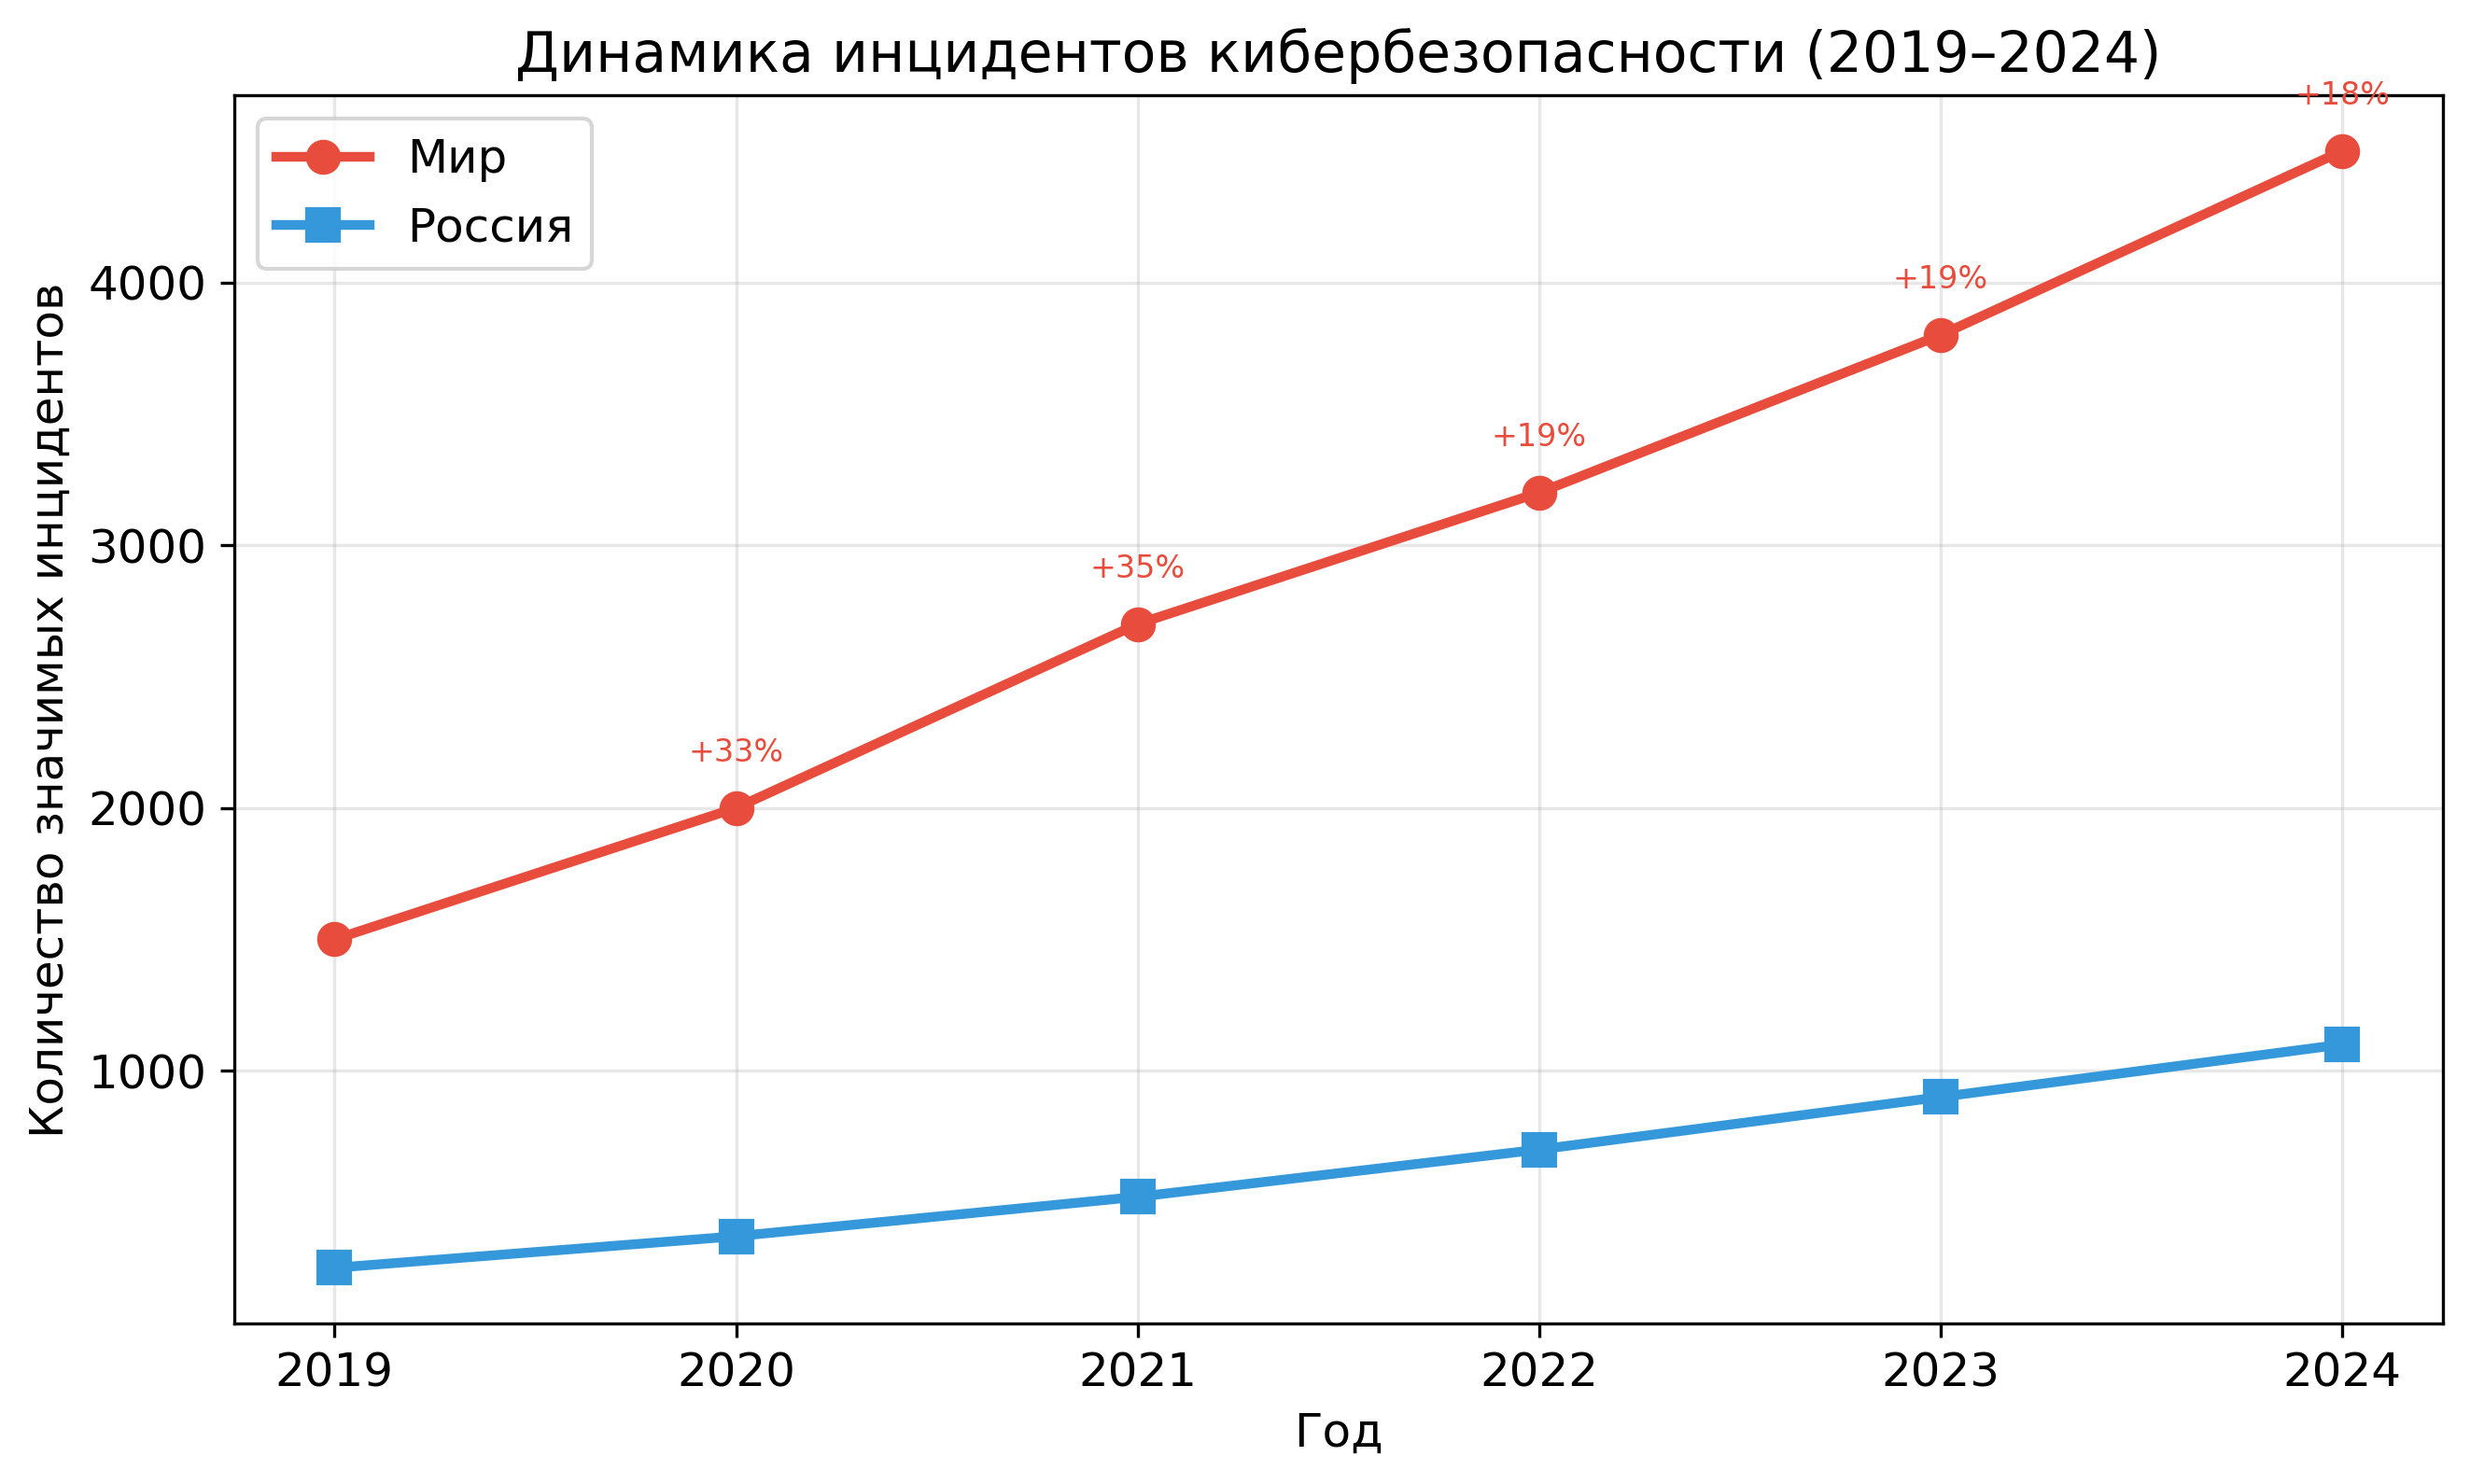
\includegraphics[width=0.85\textwidth]{images/incident_dynamics.png}
    \caption{Динамика инцидентов кибербезопасности (2019--2024)}
    \label{fig:incident_dynamics}
\end{figure}

Как видно из графика, количество значимых инцидентов в мире выросло с~1500 в 2019~году до~4500 в 2024~году, что составляет трёхкратное увеличение за пятилетний период. В российском сегменте наблюдается ещё более выраженная динамика~--- рост с~250 до~1100 инцидентов, то есть более чем в четыре раза. Данная тенденция обусловлена, в частности, геополитическими факторами, усилением активности хактивистских группировок и целенаправленными атаками на объекты критической информационной инфраструктуры Российской Федерации~[12, 13].

Анализ структуры кибератак по типам позволяет выделить наиболее распространённые векторы угроз. На рисунке~\ref{fig:attack_types} представлено распределение типов атак по данным аналитического отчёта Positive Technologies за 2024~год.

\begin{figure}[htbp]
    \centering
    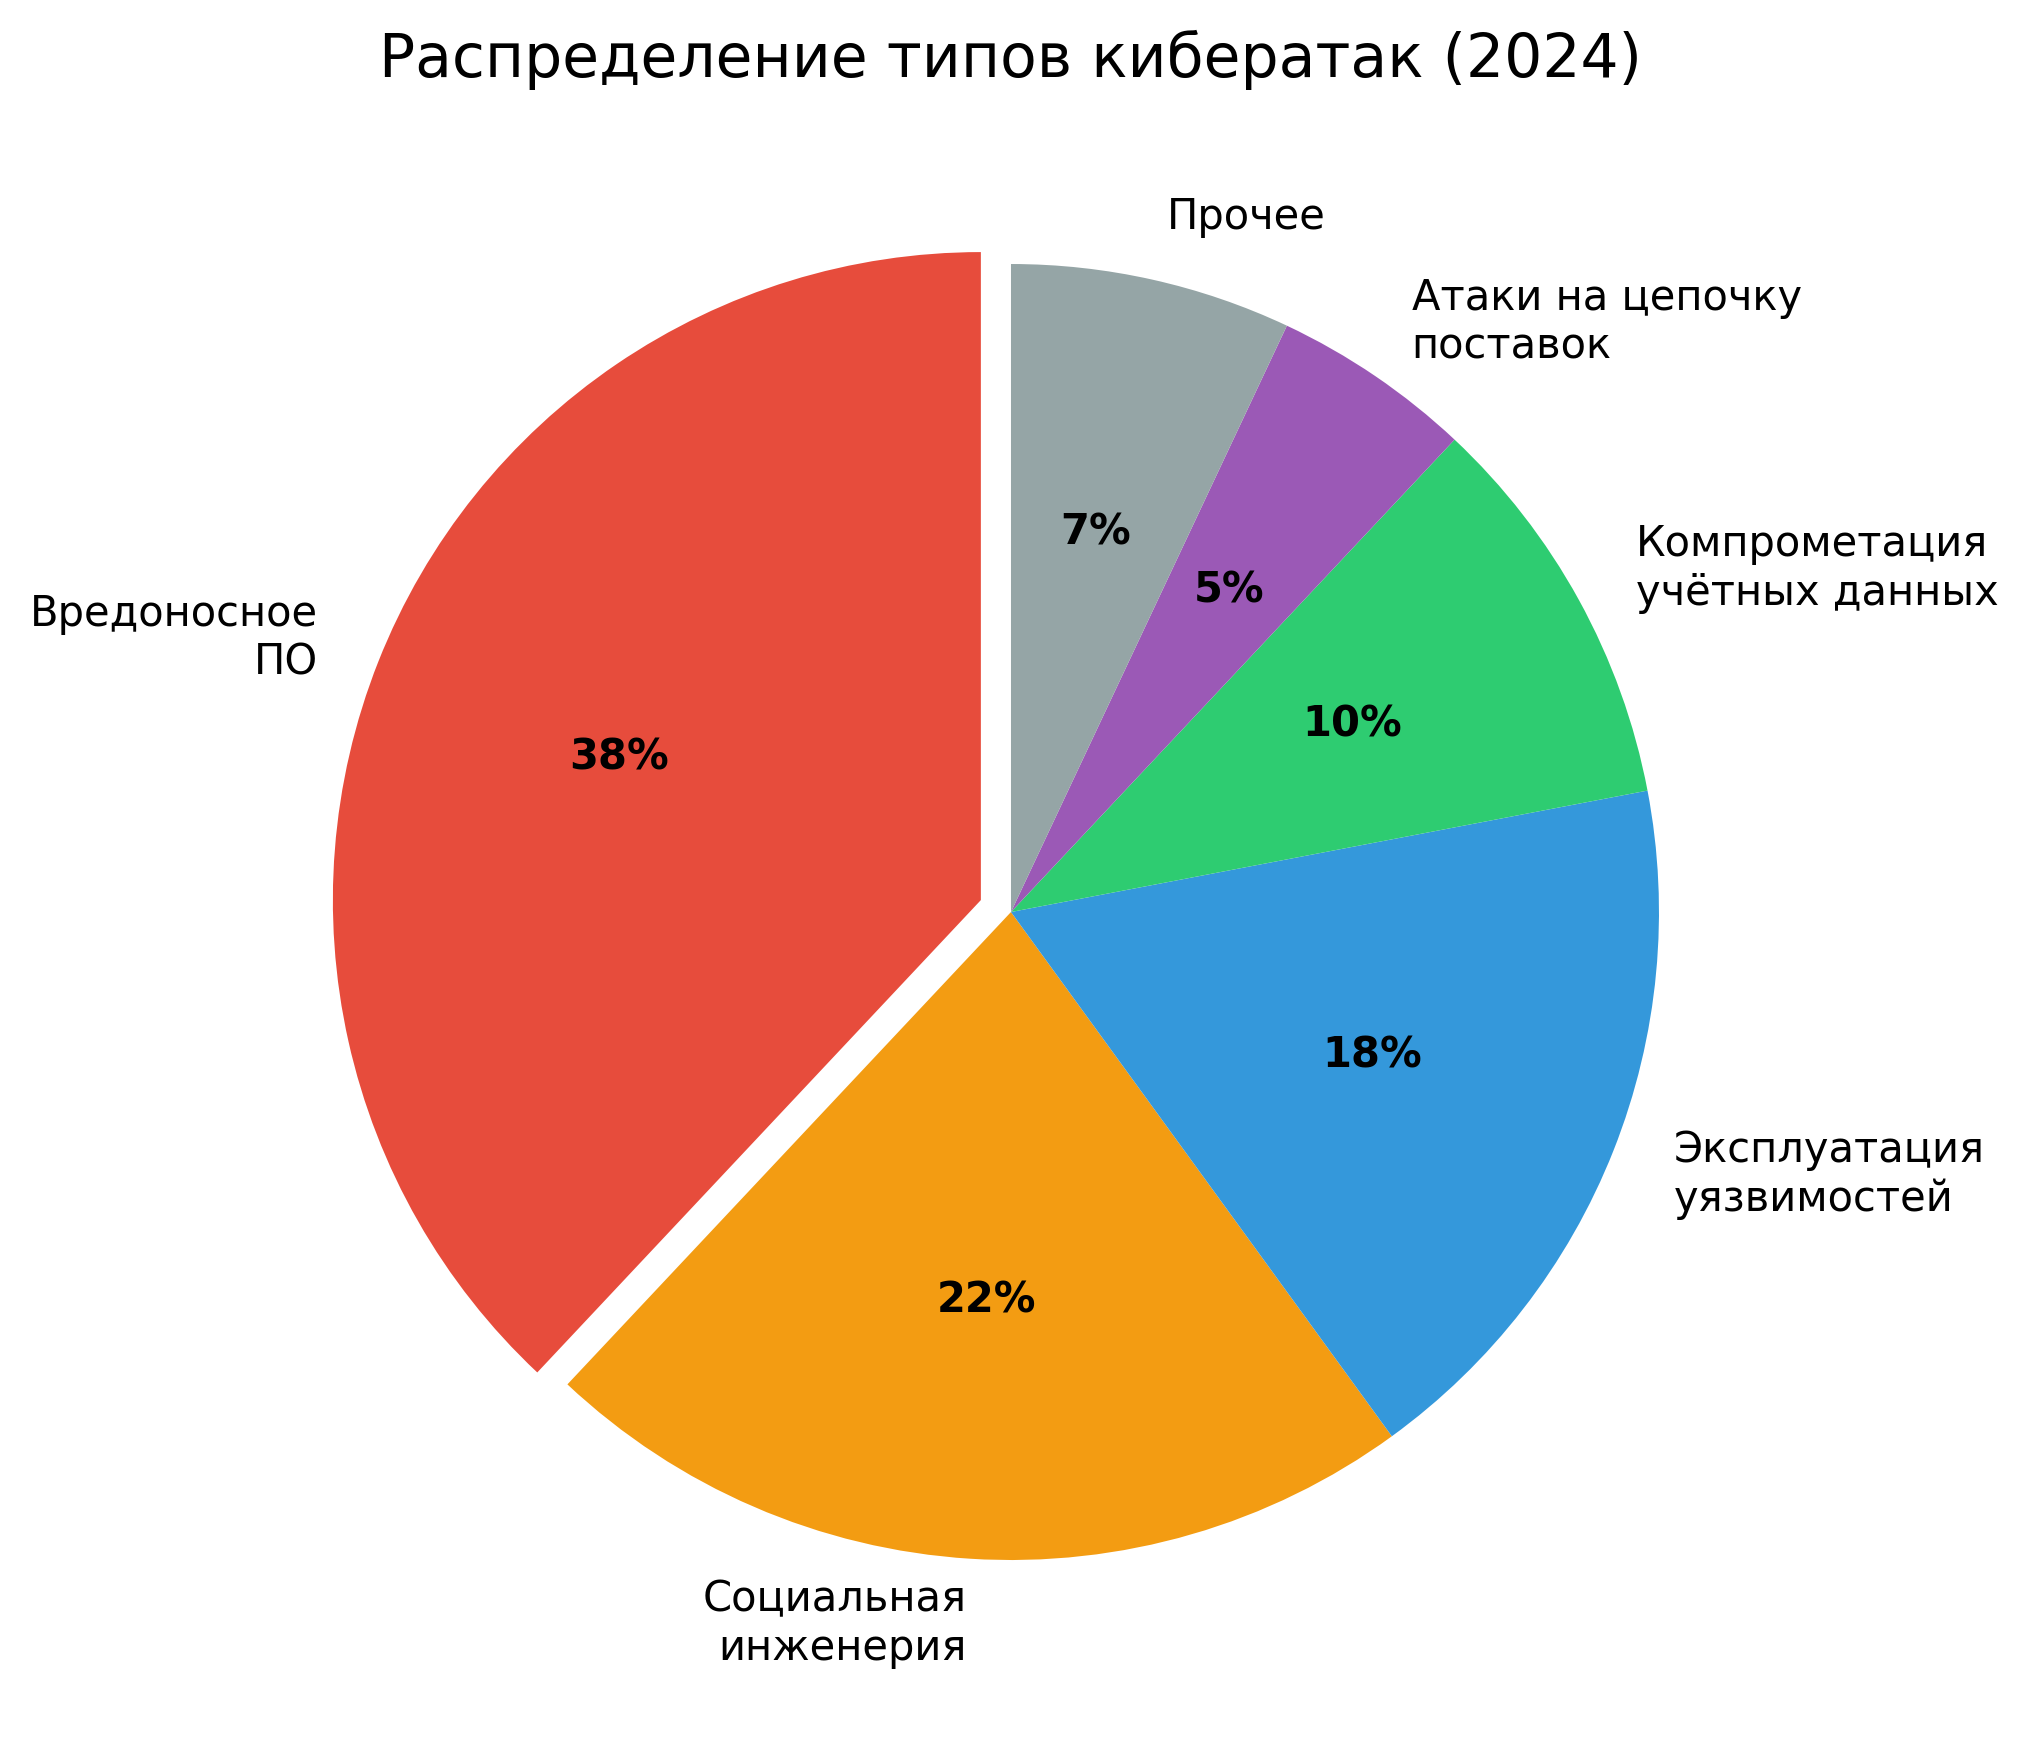
\includegraphics[width=0.75\textwidth]{images/attack_types.png}
    \caption{Распределение типов кибератак (2024)}
    \label{fig:attack_types}
\end{figure}

Доминирующим типом атак остаётся вредоносное программное обеспечение (38\,\%), включающее ransomware, трояны и бэкдоры. Социальная инженерия занимает второе место (22\,\%), что подчёркивает значимость человеческого фактора в обеспечении информационной безопасности. Эксплуатация уязвимостей программного обеспечения составляет 18\,\% инцидентов, что связано с ростом числа обнаруживаемых уязвимостей нулевого дня. Атаки на цепочку поставок (5\,\%), несмотря на относительно малую долю, характеризуются высоким потенциалом ущерба, поскольку позволяют компрометировать множество организаций через единую точку входа.

Важной тенденцией является переход от явных атак и массовых сканирований к методам low-and-slow, в рамках которых злоумышленники стремятся оставаться незаметными за счёт снижения интенсивности активности и использования стеганографических каналов передачи команд и контрольных сообщений~[11]. Это ставит новые задачи для систем киберзащиты, требующих развития механизмов выявления скрытых угроз.

\subsection{Тенденции применения стеганографии злоумышленниками}

Стеганография, как техника скрытия информации внутри иных носителей, издавна использовалась в военных и разведывательных целях, однако с развитием компьютерных технологий и сетей стала инструментом для киберпреступников. Исторические примеры применения сетевой стеганографии включают вредоносные программы Duqu и Flame~[14], а также проект ProjectSauron~[15], где была задокументирована реализация скрытых командных каналов. Современные кейсы, такие как деятельность группировки Turla, демонстрируют использование DNS-запросов в качестве стеганографического канала~[11], а также расследования Equation Group показывают сложные методы встраивания информации в TCP/IP стек~[16].

Более детальный анализ деятельности указанных группировок позволяет оценить масштаб и техническую сложность применяемых стеганографических методов. Группировка Turla (также известная как Snake, Venomous Bear, Uroburos), связываемая аналитиками с российскими спецслужбами, разработала один из наиболее изощрённых механизмов DNS-туннелирования. Вредоносное ПО данной группы формировало DNS-запросы к контролируемым злоумышленниками серверам имён, кодируя команды и эксфильтрируемые данные в полях QNAME с использованием кастомного алфавита Base64. Ключевой особенностью являлось использование легитимных DNS-резолверов организации-жертвы в качестве промежуточных узлов, что позволяло обходить ограничения межсетевого экрана на прямые DNS-запросы к внешним серверам~[11]. Для снижения вероятности обнаружения система ограничивала частоту запросов до 1--2 в минуту и варьировала длину QNAME, имитируя паттерны обращений к CDN-сервисам.

Группировка Equation Group, описанная в отчётах компании Kaspersky~[16], применяла модификацию полей TCP/IP стека для организации скрытых каналов управления имплантами. В частности, было задокументировано использование поля IP Identification для передачи однобайтовых команд, а также манипуляция порядковыми номерами TCP для кодирования четырёхбайтовых блоков данных. Особый интерес представляет применение данной группировкой техники <<двойного дна>>: первичный канал связи осуществлялся через HTTP, а стеганографический канал в TCP ISN активировался только при получении специальной команды-триггера, что существенно затрудняло его обнаружение при ретроспективном анализе трафика.

Вредоносное ПО StegoLoader, впервые обнаруженное исследователями Dell SecureWorks, представляет пример гибридного подхода: основной модуль загрузки использовал стеганографию в PNG-изображениях для доставки полезной нагрузки, однако командно-контрольный канал был реализован через манипуляцию полями ICMP Echo Request. Размер полезной нагрузки ICMP-пакетов варьировался в пределах 56--84~байт, что соответствовало типичным значениям для утилиты \texttt{ping} различных ОС, а данные размещались в последних 8--16~байтах payload.

Группировка APT29 (Cozy Bear) в рамках кампании Hammertoss использовала многоуровневую стеганографическую схему: управляющие команды кодировались в изображениях, публикуемых на платформе Twitter (ныне X), а адреса серверов для эксфильтрации извлекались из временных меток публикаций. Данный подход демонстрирует тенденцию к использованию легитимных социальных платформ в качестве промежуточного звена стеганографической коммуникации, что существенно усложняет блокировку C2-каналов на уровне сетевой инфраструктуры.

Обобщённая характеристика APT-группировок, применяющих стеганографические техники, представлена на рисунке~\ref{fig:apt_stego}. Диаграмма отражает продолжительность известной активности каждой группировки и используемые ею стеганографические методы.

\begin{figure}[htbp]
    \centering
    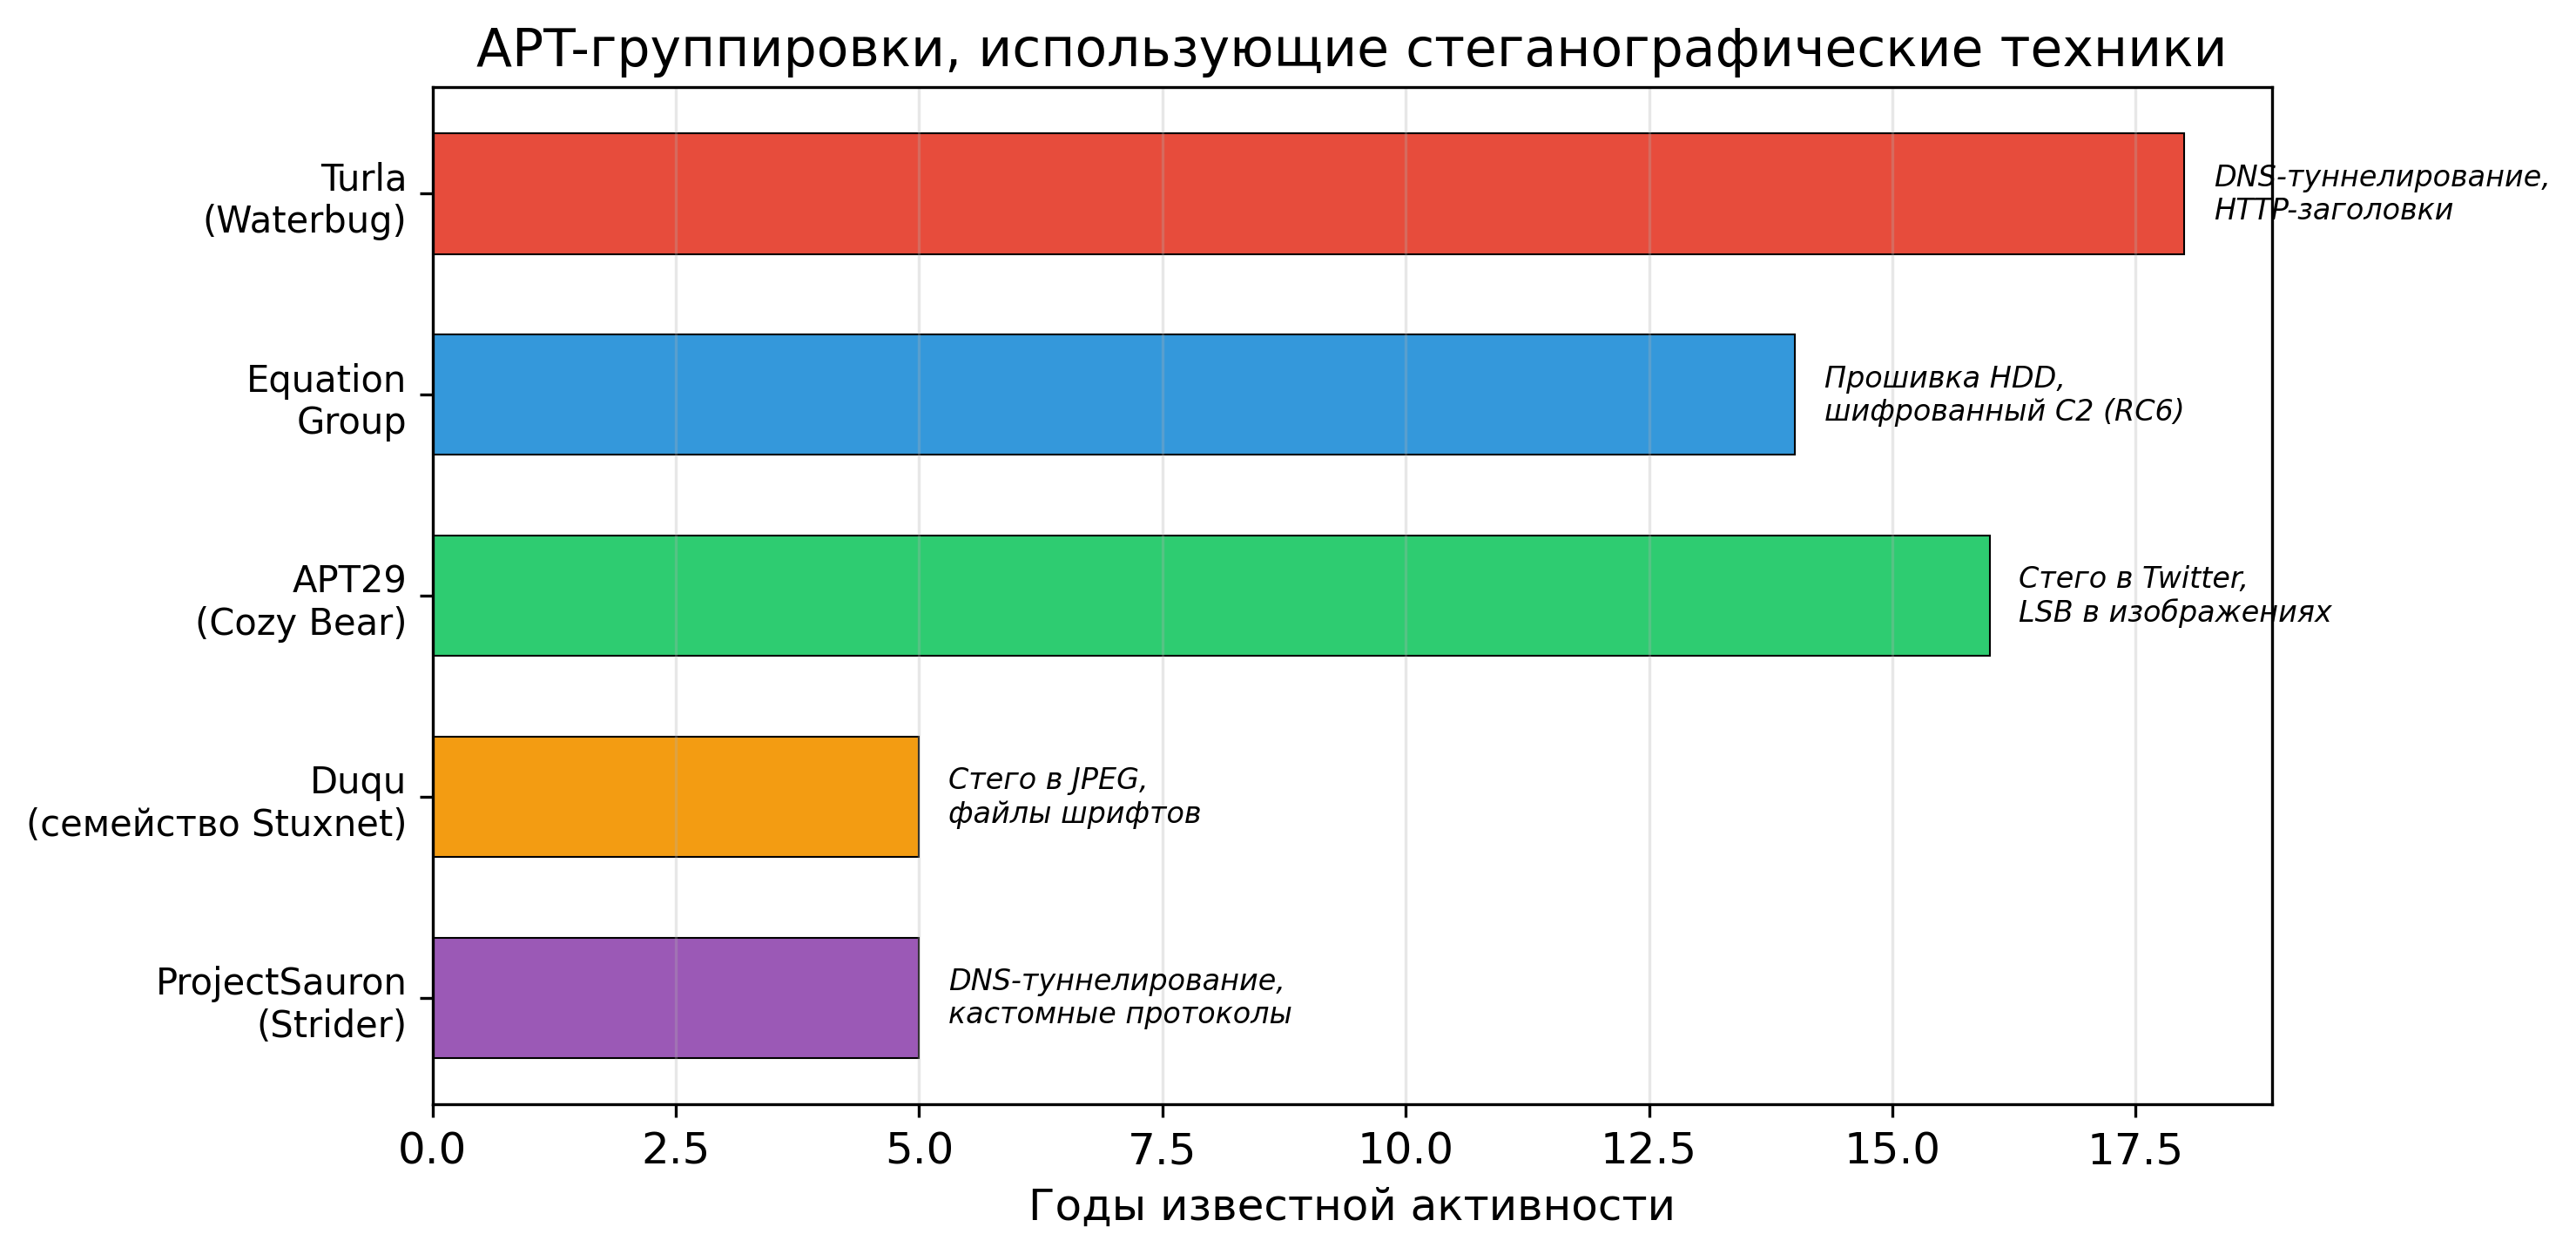
\includegraphics[width=0.9\textwidth]{images/apt_stego.png}
    \caption{APT-группировки, использующие стеганографические техники}
    \label{fig:apt_stego}
\end{figure}

Как видно из диаграммы, некоторые из рассмотренных группировок ведут активную деятельность на протяжении более 15~лет (Turla~--- с 2008~года, Equation Group~--- с 2001~года), что свидетельствует о высокой эффективности стеганографических методов сокрытия и трудности их обнаружения традиционными средствами защиты. Разнообразие применяемых техник~--- от DNS-туннелирования и модификации TCP/IP-заголовков до стеганографии в изображениях~--- указывает на необходимость комплексного подхода к обнаружению, сочетающего статистический анализ, машинное обучение и сигнатурные методы.

Рост популярности стеганографии в сетевых протоколах обусловлен рядом факторов:

\begin{enumerate}[label=\arabic*)]
    \item обход систем глубокого анализа трафика (DPI), основанных на детектировании сигнатур;
    \item способность маскироваться под обычный сетевой трафик, снижая вероятность обнаружения;
    \item отсутствие сквозного шифрования заголовков протоколов TCP/IP, что упрощает манипуляции с ними;
    \item широкий выбор полей и опций, пригодных для стеганографии.
\end{enumerate}

\subsection{Влияние скрытых каналов на безопасность корпоративных сетей}

Скрытые каналы связи (covert channels) были впервые формализованы в работах Lampson (1973)~[17] и разделены на два основных типа: каналы хранения (covert storage channels) и каналы времени (covert timing channels). В контексте сетевых протоколов каналы хранения реализуются через встраивание данных в поля заголовков или полезной нагрузки пакетов, а каналы времени~--- через манипуляцию интервалами передачи пакетов.

Сравнительная характеристика типов скрытых каналов по ключевым параметрам представлена на рисунке~\ref{fig:channel_classification}. Оценка производится по трём критериям: пропускная способность, скрытность и сложность обнаружения.

\begin{figure}[htbp]
    \centering
    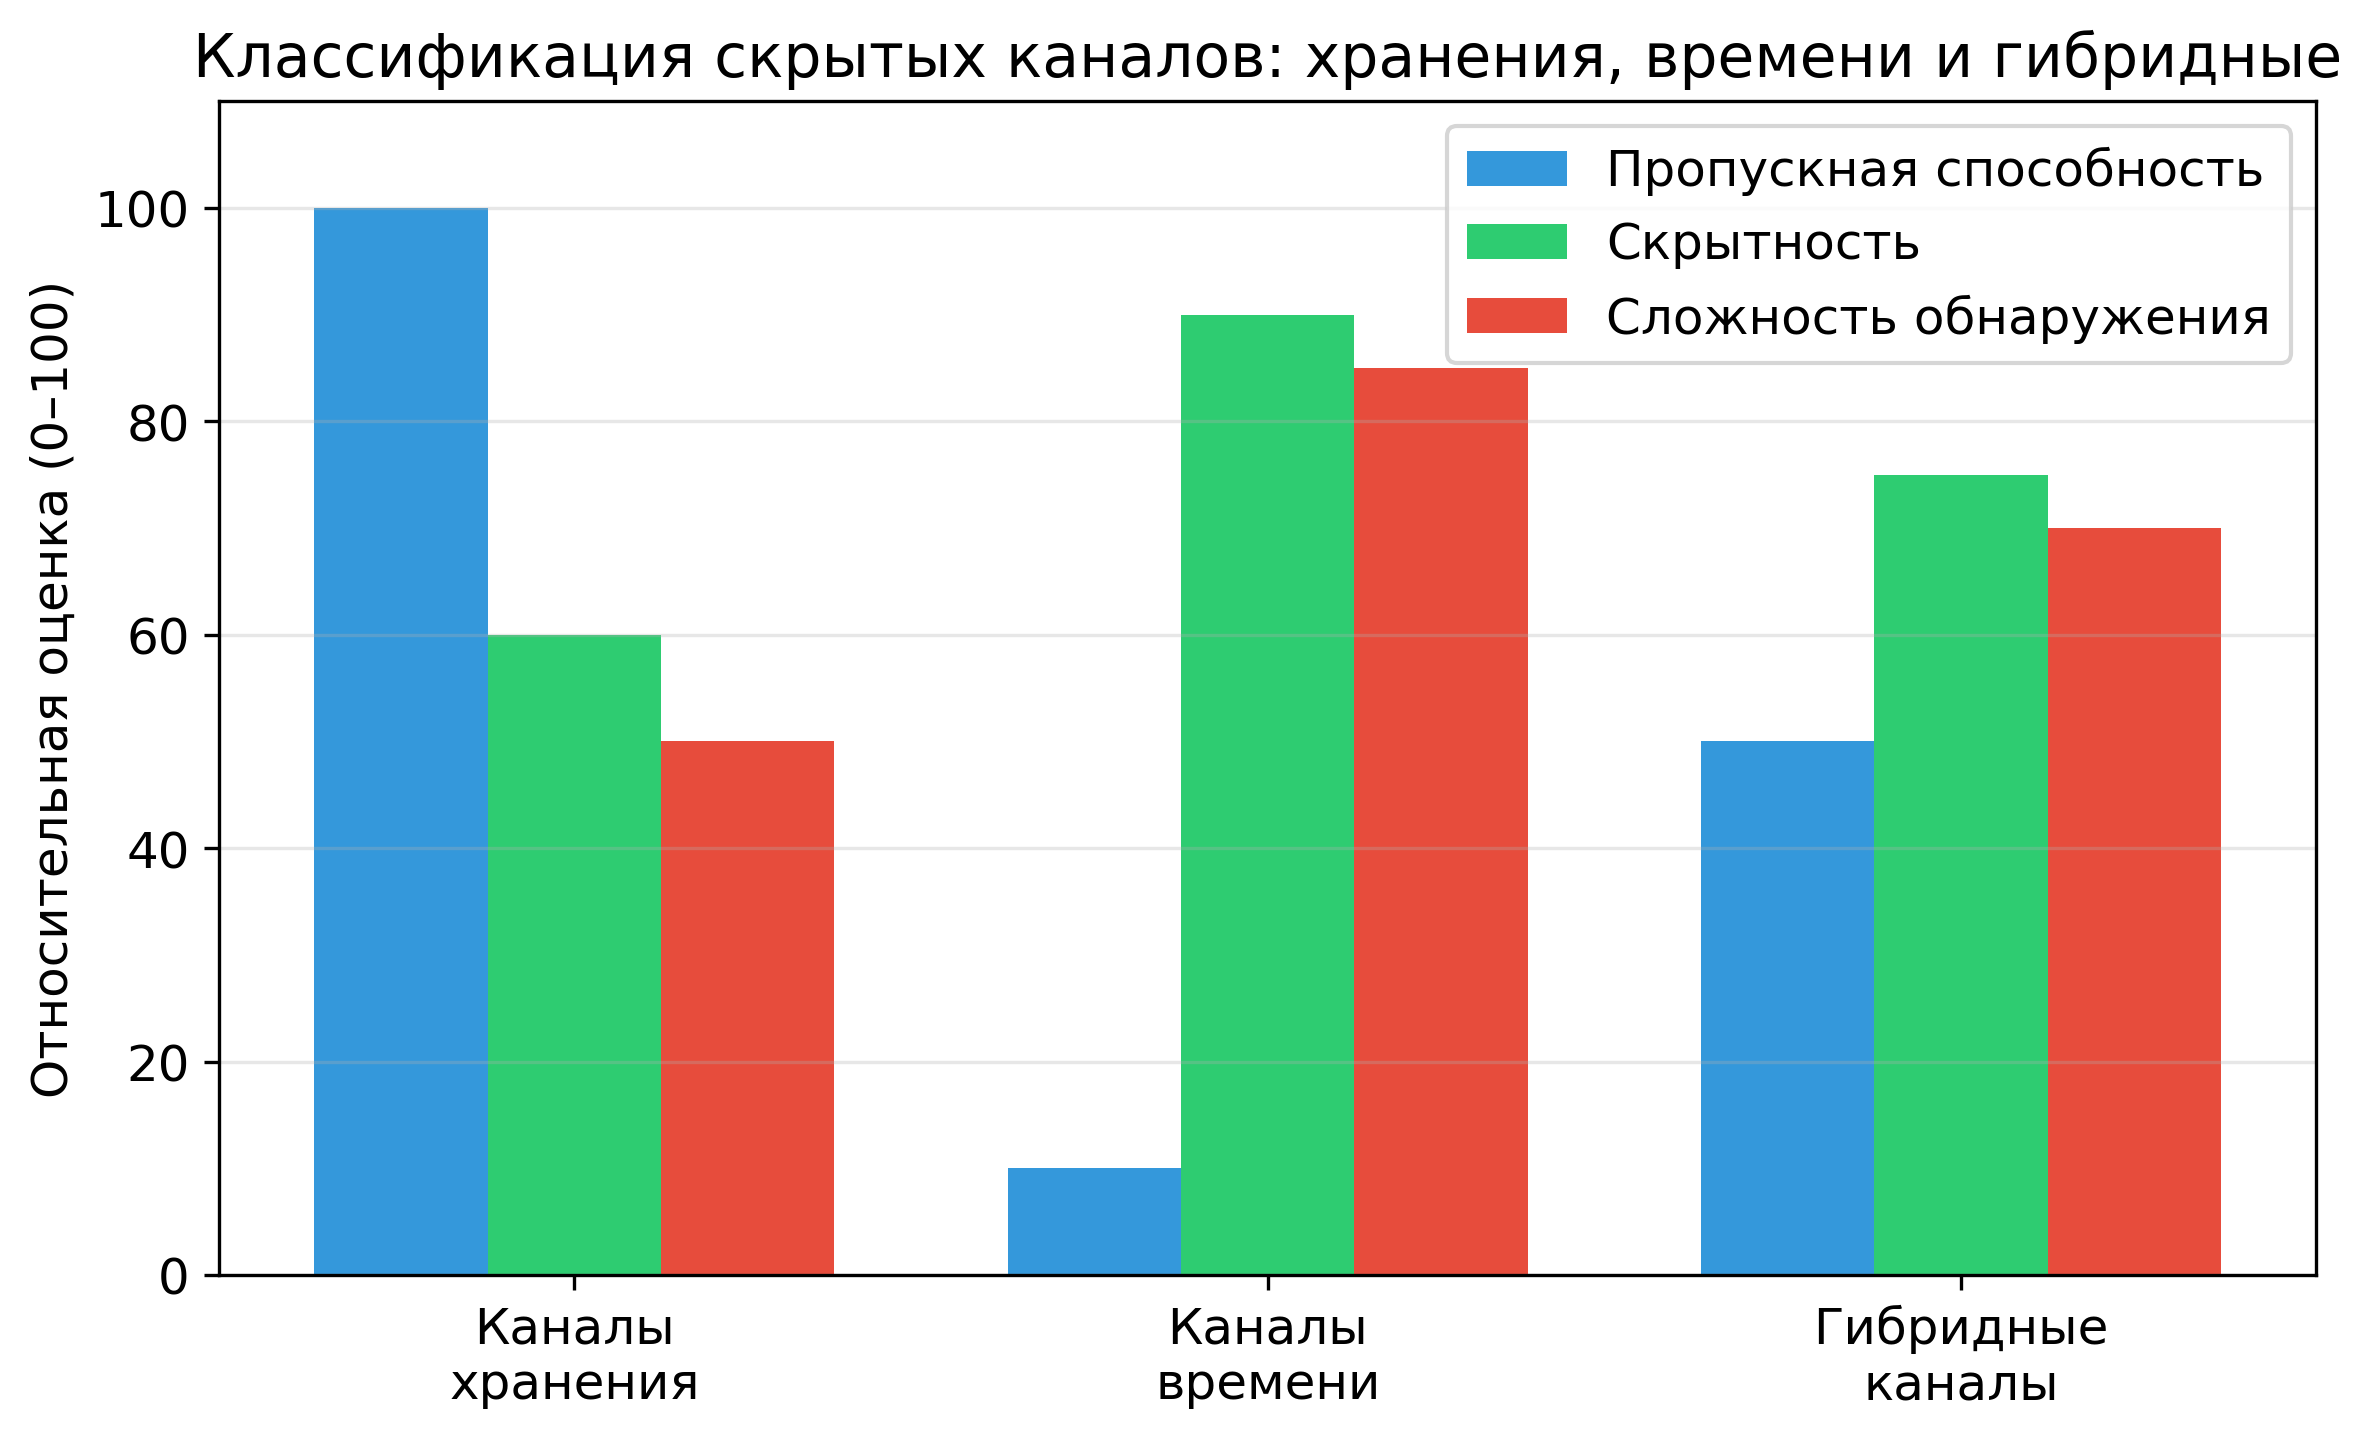
\includegraphics[width=0.8\textwidth]{images/channel_classification.png}
    \caption{Классификация скрытых каналов: хранения, времени и гибридные}
    \label{fig:channel_classification}
\end{figure}

Каналы хранения обладают наибольшей пропускной способностью, поскольку позволяют встраивать данные непосредственно в поля пакетов, однако их скрытность относительно невысока~--- модифицированные поля могут быть выявлены статистическим анализом. Каналы времени, напротив, характеризуются высокой скрытностью и сложностью обнаружения, но их пропускная способность существенно ограничена, так как информация кодируется через межпакетные задержки. Гибридные каналы, комбинирующие оба подхода, представляют компромисс между пропускной способностью и скрытностью, однако их реализация значительно сложнее.

Использование таких скрытых каналов представляет серьёзные риски для безопасности корпоративных сетей, включая:

\begin{enumerate}[label=\arabic*)]
    \item эксфильтрацию конфиденциальных данных в обход систем контроля доступа (NAC) и межсетевых экранов;
    \item реализацию командно-контрольных (C2) каналов для управления вредоносным ПО;
    \item затруднение обнаружения и идентификации атакующих активностей.
\end{enumerate}

Помимо непосредственных технических рисков, скрытые каналы создают значительные проблемы для процессов реагирования на инциденты. При расследовании компрометации организации аналитики, как правило, фокусируются на анализе известных индикаторов компрометации (IoC) --- IP-адресов, доменных имён, хешей файлов. Стеганографические каналы, использующие легитимные протоколы и не создающие новых сетевых соединений, не порождают характерных IoC и могут оставаться незамеченными даже при детальном ретроспективном анализе трафика. Это обстоятельство значительно увеличивает среднее время обнаружения инцидента (Mean Time to Detect, MTTD), которое, по данным отчёта IBM Cost of a Data Breach~[12], составляет 204~дня для атак с использованием продвинутых техник сокрытия.

Кроме того, наличие скрытых каналов в корпоративной сети ставит под сомнение эффективность контрольных мер, основанных на мониторинге сетевого трафика. Системы класса DLP (Data Loss Prevention), контролирующие исходящий трафик на предмет утечки конфиденциальных данных, оказываются неэффективными при стеганографической эксфильтрации, поскольку данные передаются в полях заголовков, не подвергаемых содержательному анализу~[13]. Аналогичным образом, системы SIEM (Security Information and Event Management), агрегирующие журналы событий, не фиксируют манипуляции с полями заголовков на уровне отдельных пакетов.

Таким образом, понимание и обнаружение скрытых каналов является ключевой задачей обеспечения комплексной защиты информационных систем.

\subsection{Нормативно-правовые аспекты обнаружения скрытых каналов}

Проблема обнаружения скрытых каналов в сетевых протоколах имеет не только техническое, но и нормативно-правовое измерение. В Российской Федерации вопросы защиты информации в информационных системах регулируются комплексом нормативных актов и руководящих документов.

Федеральная служба по техническому и экспортному контролю (ФСТЭК России) определяет требования к защите информации в информационных системах различных классов. Приказ ФСТЭК России №~17 от 11~февраля 2013~года <<Об утверждении требований о защите информации, не составляющей государственную тайну, содержащейся в государственных информационных системах>> устанавливает обязательность применения мер по обнаружению вторжений (ОБС) и анализу защищённости (АНЗ) для информационных систем 1-го и 2-го классов защищённости. В контексте данных требований скрытые каналы представляют собой класс угроз, для противодействия которым необходимы специализированные средства анализа.

Приказ ФСТЭК России №~239 от 25~декабря 2017~года <<Об утверждении требований по обеспечению безопасности значимых объектов критической информационной инфраструктуры Российской Федерации>> определяет меры по защите значимых объектов КИИ. Для объектов 1-й категории значимости предусматривается необходимость контроля информационных потоков и обнаружения скрытых каналов утечки информации. Методический документ ФСТЭК <<Меры защиты информации в государственных информационных системах>> конкретизирует данные требования, указывая на необходимость анализа сетевого трафика с целью выявления нехарактерных информационных потоков.

Федеральный закон №~187-ФЗ <<О безопасности критической информационной инфраструктуры Российской Федерации>> от 26~июля 2017~года обязывает субъектов КИИ обеспечивать непрерывность функционирования объектов и информирование ГосСОПКА о компьютерных инцидентах. Использование злоумышленниками стеганографических каналов для управления вредоносным ПО на объектах КИИ создаёт угрозу нарушения их функционирования, что обуславливает необходимость разработки и внедрения средств обнаружения таких каналов.

На международном уровне стандарт ISO/IEC~27001:2022 в рамках контрольных мер приложения~A (A.8.16 <<Monitoring activities>>) предусматривает мониторинг сетевого трафика с целью выявления аномалий, в том числе скрытых каналов. Стандарт NIST~SP~800-53~Rev.~5 включает контрольную меру SC-31 <<Covert Channel Analysis>>, непосредственно адресующую проблему анализа скрытых каналов в информационных системах и рекомендующую проведение систематического анализа системных интерфейсов на предмет наличия скрытых каналов.

Таким образом, разработка инструментов обнаружения стеганографических скрытых каналов в сетевых протоколах является не только научно-исследовательской задачей, но и необходимым условием обеспечения соответствия информационных систем требованиям регуляторов в области информационной безопасности.

\subsection{Роль протоколов TCP/IP как носителей скрытой информации}

Стек протоколов TCP/IP остаётся основным стандартом передачи данных в глобальной сети. Его широкое распространение и отсутствие шифрования некоторых заголовочных полей делают его удобной средой для реализации сетевой стеганографии~[1, 3].

Основными полями и элементами протоколов, подходящими для сокрытия данных, являются:

\begin{enumerate}[label=\arabic*)]
    \item \textbf{IP Identification (IP ID)} --- 16-битное поле в заголовке IPv4 (RFC 791~[3]), предназначенное для идентификации фрагментов пакетов. Использование этого поля позволяет встраивать 2 байта данных на пакет, при этом необходимо учитывать особенности поведения операционной системы, такие как инкрементальное или случайное формирование значения~[3].
    \item \textbf{TCP Initial Sequence Number (ISN)} --- 32-битное поле, устанавливаемое при инициации TCP-соединения (RFC 793~[4]), однако с применением рандомизации (RFC 6528~[18]) для повышения безопасности. Встраивание данных требует аккуратной обработки и обхода защитных механизмов.
    \item \textbf{TCP Timestamp (TSval)} --- 32-битное поле в опции TCP Timestamp (RFC 7323~[7]), используемое для оценки времени прохождения пакетов. Для корректной работы метод должен учитывать политики операционной системы относительно timestamps (например, net.ipv4.tcp\_timestamps = 1).
    \item \textbf{ICMP Echo Request Payload} --- поле данных в ICMP-пакетах (RFC 792~[5]), объёмом до 1472 байт (с учётом MTU Ethernet), предоставляющее значительный объём для скрытия информации, хотя и менее скрытное из-за отсутствия шифрования и возможности анализа размера.
    \item \textbf{DNS QNAME} --- имя доменного запроса в протоколе DNS (RFC 1035~[6]), длина до 255 байт, с возможностью кодирования в base32 и маскировкой под легитимные DNS-запросы.
\end{enumerate}

Существенным фактором, определяющим возможности и ограничения стеганографического использования указанных полей, является различие в поведении операционных систем при формировании значений заголовков пакетов.

В отношении поля IP~ID наблюдаются принципиальные различия между операционными системами. Ядро Linux (начиная с версии 4.1) использует алгоритм генерации IP~ID на основе хеш-функции от адреса назначения, что приводит к формированию отдельной инкрементальной последовательности для каждого уникального адреса. Для пакетов с установленным флагом DF (Don't Fragment) ядро Linux может устанавливать IP~ID в значение~0, что является допустимым согласно RFC~6864~[3]. Операционные системы семейства Windows (начиная с Windows~Vista) используют глобальный инкрементальный счётчик IP~ID, увеличиваемый на единицу для каждого исходящего пакета вне зависимости от адреса назначения. Операционная система FreeBSD реализует случайную генерацию IP~ID с использованием криптографически стойкого генератора. Указанные различия имеют непосредственное значение для стеганографии: замена значения IP~ID на произвольное значение наиболее заметна в среде Windows с её предсказуемой инкрементальной моделью, и наименее заметна в FreeBSD, где значения и без того являются случайными.

В отношении начальных порядковых номеров TCP (ISN) все современные операционные системы реализуют рандомизацию в соответствии с RFC~6528~[18], однако конкретные алгоритмы различаются. Ядро Linux использует функцию SipHash от четвёрки значений (IP-адреса и порты источника и назначения) с добавлением счётчика, инкрементируемого каждые 64~наносекунды. Windows использует аналогичный подход, однако с собственной реализацией хеш-функции и другим интервалом инкрементирования. Для стеганографии в TCP~ISN критическим является тот факт, что полная замена значения ISN нарушает корреляцию между значениями ISN для последовательных соединений к одному серверу, что может быть выявлено при статистическом анализе.

Поведение TCP Timestamp также зависит от операционной системы. В Linux начальное значение TSval формируется на основе значения \texttt{jiffies} --- внутреннего счётчика ядра с частотой, определяемой конфигурацией \texttt{CONFIG\_HZ} (типичные значения~--- 100, 250 или 1000~Гц). Таким образом, TSval инкрементируется с предсказуемой частотой, и любое отклонение от линейного роста может служить индикатором стеганографической модификации. В Windows TCP Timestamp инкрементируется с частотой 100~Гц (шаг 10~мс). Стеганографическая замена TSval на произвольное значение нарушает монотонность последовательности, что является обнаруживаемой аномалией.

Для протокола ICMP различия между ОС проявляются в размере полезной нагрузки по умолчанию: утилита \texttt{ping} в Linux отправляет 56~байт данных (в итоге 64~байта с заголовком ICMP), в Windows~--- 32~байта, а в macOS~--- также 56~байт. Содержимое payload по умолчанию также различается: Linux заполняет его временной меткой и инкрементируемыми байтами, Windows использует повторяющуюся последовательность \texttt{abcdefghijklmnop...}. Стеганографическое использование ICMP payload требует имитации паттерна конкретной ОС для снижения вероятности обнаружения.

Данные поля образуют базу для создания эффективных и скрытных стеганографических каналов в сетевых коммуникациях.


\newpage

%% Глава 2
%%% chapter2.tex — Глава 2
\section{Теоретические основы сетевой стеганографии и обнаружения вредоносных вложений}

В предыдущей главе обоснована актуальность задачи обнаружения сетевой стеганографии в условиях современного ландшафта киберугроз и выделены конкретные поля заголовков TCP/IP, пригодные для встраивания скрытой информации. В настоящей главе формализуются теоретические основы как методов сокрытия данных в этих полях, так и методов их обнаружения~--- что позволяет в дальнейшем перейти к программной реализации соответствующих подсистем.

\subsection{Основные понятия и классификация методов стеганографии}

Стеганография --- это метод скрытой передачи информации путём встраивания её в другой, внешне нейтральный контейнер, с целью скрыть факт коммуникации~[2]. В отличие от криптографии, обеспечивающей конфиденциальность содержимого сообщения, стеганография скрывает само существование передаваемых данных. Сочетание обоих подходов обеспечивает максимальный уровень защиты: даже при обнаружении скрытого канала содержимое остаётся нечитаемым без ключа расшифрования.

По среде передачи стеганографические методы классифицируются следующим образом~[11]:

\begin{enumerate}[label=\arabic*)]
  \item \textbf{Текстовая стеганография} --- встраивание информации в текстовые файлы с использованием невидимых символов, пробелов, особенностей шрифтов.
  \item \textbf{Графическая стеганография} --- сокрытие данных в изображениях путём модификации младших значащих бит (LSB) пикселей, частотных компонент или цветовых каналов.
  \item \textbf{Аудио- и видеостеганография} --- кодирование данных в аудиопотоках или видеофайлах с использованием психоакустических моделей и временны\'{х} характеристик.
  \item \textbf{Сетевая стеганография} --- внедрение информации в поля и поведение сетевых протоколов при формировании и передаче пакетов TCP/IP.
\end{enumerate}

По методам встраивания выделяют три основных подхода:

\begin{enumerate}[label=\arabic*)]
  \item \textbf{С заменой (substitution)} --- внедрение информации путём замены битов или полей исходного контейнера на скрытые данные. В сетевой стеганографии этот метод применяется при модификации полей заголовков (IP~ID, TCP~ISN).
  \item \textbf{С расширением (extension)} --- добавление дополнительных полей или данных, увеличивающих объём контейнера. Например, включение дополнительных опций TCP или расширенных DNS-записей.
  \item \textbf{С генерацией (generation)} --- создание специально сформированного контейнера, изначально содержащего скрытые данные. Примером является генерация DNS-запросов с закодированными в QNAME данными.
\end{enumerate}

Формальная модель стеганографической системы включает следующие компоненты~[11, 12]:

\begin{enumerate}[label=\arabic*)]
  \item \textbf{контейнер (Cover)} --- исходный объект, в который внедряется сообщение;
  \item \textbf{стеганографический ключ} --- секретный параметр, определяющий алгоритм и место встраивания;
  \item \textbf{функция встраивания $E(C, M, K) \to S$} --- преобразование контейнера $C$, сообщения $M$ и ключа $K$ в стегоконтейнер $S$;
  \item \textbf{функция извлечения $D(S, K) \to M$} --- восстановление скрытого сообщения из стегоконтейнера;
  \item \textbf{нарушитель (Warden)} --- субъект, осуществляющий пассивный или активный анализ с целью обнаружения или уничтожения скрытой информации.
\end{enumerate}

\subsection{Сравнительный анализ сетевой и контейнерной стеганографии}

При выборе метода скрытой передачи данных по сети возникает вопрос: что целесообразнее --- встраивать информацию в поля сетевых протоколов или использовать классическую контейнерную стеганографию, передавая по сети изображения, аудио- и видеофайлы с внедрёнными данными? Оба подхода имеют свои преимущества и ограничения, и выбор между ними определяется конкретным сценарием применения.

\textbf{Контейнерная стеганография} (встраивание в изображения, аудио, видео) обладает высокой ёмкостью: метод LSB (Least Significant Bit) позволяет встроить до 12{,}5\,\% от объёма изображения (1~бит на канал на пиксель при 3~каналах), а частотные методы (DCT, DWT) обеспечивают ёмкость порядка 5--10\,\% при лучшей устойчивости к стегоанализу. Для изображения размером 1~МБ это означает возможность передачи 50--125~КБ скрытых данных в одном файле. Видеоконтейнеры ещё более ёмки: в потоке 720p~(30~fps) теоретически возможна скрытая передача данных со скоростью до нескольких Мбит/с.

Однако контейнерная стеганография при передаче по сети имеет существенные недостатки. Во-первых, необходим канал передачи контейнеров --- HTTP, FTP, электронная почта или мессенджер, что создаёт дополнительные метаданные (URL, отправитель, получатель, временны\'{е} метки), анализируемые системами DLP и SIEM. Во-вторых, промежуточные сервисы часто выполняют перекодирование мультимедиа: социальные сети сжимают изображения (JPEG с потерей качества), мессенджеры конвертируют видео, CDN-серверы оптимизируют контент. Перекодирование разрушает встроенные данные, если не использованы устойчивые (robust) алгоритмы встраивания. В-третьих, регулярная передача изображений или видеофайлов между определёнными узлами сети может привлечь внимание аналитиков безопасности, особенно если данные узлы обычно не обмениваются мультимедийным контентом.

\textbf{Сетевая стеганография} (встраивание в заголовки протоколов) обладает принципиально иными характеристиками. Её главное преимущество --- отсутствие дополнительного контейнера: скрытые данные передаются непосредственно в служебных полях пакетов, которые генерируются при любом сетевом взаимодействии. Это означает, что стеганографическая передача не создаёт новых информационных потоков и не требует дополнительных приложений или протоколов. Пакеты ICMP, DNS-запросы, TCP-соединения являются штатными элементами сетевой активности любой организации, и их наличие само по себе не вызывает подозрений.

К недостаткам сетевой стеганографии относятся низкая ёмкость каналов (от 2~до 1470~байт на пакет, что на порядки меньше, чем у контейнерной стеганографии), зависимость от сетевой инфраструктуры (NAT, межсетевые экраны, прокси-серверы могут модифицировать или отбрасывать пакеты) и более строгие требования к синхронизации между отправителем и получателем.

Таким образом, сетевая стеганография наиболее целесообразна в следующих сценариях: передача малых объёмов критически важных данных (криптографические ключи, управляющие команды, координаты C2-серверов --- типичные объёмы до нескольких килобайт); работа в средах с жёстким контролем контента (где передача мультимедийных файлов ограничена или мониторируется); необходимость полной маскировки факта коммуникации (отсутствие дополнительных файлов и соединений). Контейнерная стеганография, напротив, предпочтительна для передачи больших объёмов данных (документы, базы данных) через каналы, где мультимедийный трафик является нормой (социальные сети, мессенджеры, электронная почта).

В рамках настоящей работы выбор в пользу сетевой стеганографии обусловлен её актуальностью для задач кибербезопасности: именно сетевые скрытые каналы используются APT-группировками для управления имплантами и эксфильтрации данных в корпоративных средах с контролируемым сетевым периметром. Разработка модуля обнаружения таких каналов представляет непосредственную практическую ценность для защиты информационных систем.

\subsection{Методы сокрытия данных в заголовках сетевых протоколов}

Рассмотрим подробнее алгоритмы встраивания данных для каждого из пяти каналов, реализованных в системе \texttt{NetStego}.

\subsubsection{ICMP Payload}

Поле полезной нагрузки ICMP Echo Request (тип~8, код~0) согласно RFC~792~[5] не имеет строго определённого формата содержимого --- стандарт лишь требует, чтобы данные, отправленные в запросе, были возвращены в ответе. Это позволяет использовать до 1472~байт для встраивания скрытых данных при стандартном MTU Ethernet~[1].

Алгоритм встраивания состоит в прямом размещении данных в поле полезной нагрузки ICMP-пакета с добавлением двухбайтового префикса длины для указания объёма полезных данных. Данный канал обеспечивает наибольшую пропускную способность, однако легко обнаруживается при анализе размера и содержимого ICMP-пакетов~[11].

Основными ограничениями канала ICMP Payload являются следующие. Во-первых, многие корпоративные межсетевые экраны блокируют ICMP-трафик или ограничивают его частоту, что снижает доступность канала. Во-вторых, нестандартный размер полезной нагрузки ICMP-пакета (например, 1470~байт вместо типичных 56~или 32~байт) является явным индикатором аномалии. В-третьих, содержимое payload не шифруется на уровне протокола, и системы DPI могут выполнять содержательный анализ данных. Для повышения скрытности канала рекомендуется ограничивать размер payload значениями, характерными для конкретной ОС отправителя, а также использовать предварительное шифрование данных, что реализовано в системе \texttt{NetStego} посредством AES-256-GCM.

Граничные случаи при работе с данным каналом включают обработку пакетов с нулевой полезной нагрузкой, пакетов, превышающих MTU сети (что приводит к фрагментации на уровне IP и потенциальной потере данных при отбрасывании фрагментов), а также ситуацию, когда промежуточный маршрутизатор модифицирует содержимое ICMP payload (что возможно при использовании NAT с поддержкой ICMP ALG).

\subsubsection{IP Identification}

Поле Identification в IPv4-заголовке (16~бит) определено в RFC~791~[3] и предназначено для идентификации фрагментов датаграммы. При отсутствии фрагментации данное поле не несёт семантической нагрузки для получателя и может быть использовано для передачи 2~байт данных на пакет.

Необходимо учитывать, что операционные системы формируют значение IP~ID различными способами: инкрементально (последовательное увеличение на единицу), случайно или на основе хеш-функции. Стеганографическая модификация IP~ID может быть обнаружена путём статистического анализа распределения значений (критерий $\chi^2$)~[11].

Алгоритм встраивания в системе \texttt{NetStego} использует IP~ID для передачи 2~байт данных в каждом ICMP Echo Request пакете. Поскольку канал имеет низкую ёмкость, фреймированный поток данных разбивается на множество пакетов: для передачи 1~КБ данных требуется примерно 587~пакетов. Для обозначения конца потока используется маркерный пакет с IP~ID~=~0xFFFF, содержащий в payload двухбайтовое значение длины последнего фрагмента. Данный маркер выбран потому, что вероятность его случайного появления в нормальном трафике крайне мала (1~из 65535 для каждого пакета), а при инкрементальной генерации IP~ID значение 0xFFFF появляется лишь один раз за полный цикл.

Ограничения канала IP~ID включают невозможность передачи данных через NAT-устройства, которые могут перезаписывать поле IP~ID в процессе трансляции адресов. Кроме того, RFC~6864 допускает установку IP~ID в~0 для нефрагментируемых пакетов, и некоторые промежуточные устройства могут нормализовать данное поле.

\subsubsection{TCP Initial Sequence Number}

Начальный порядковый номер TCP-сегмента (ISN) --- 32-битное поле, устанавливаемое при инициации соединения в SYN-пакете~[4]. Согласно RFC~6528~[10], современные ОС используют криптографически стойкую рандомизацию ISN:
\begin{equation}
\text{ISN} = M + F(\text{sip}, \text{sport}, \text{dip}, \text{dport}, K),
\label{eq:isn_rfc6528}
\end{equation}
где $M$ --- счётчик с интервалом 4~микросекунды, $F$ --- псевдослучайная функция, $K$ --- секретный ключ ОС~[10]. Встраивание данных в ISN осуществляется путём полной замены значения, что требует подавления RST-пакетов ядра ОС с помощью правил межсетевого экрана.

В реализации системы \texttt{NetStego} каждый SYN-пакет содержит 4~байта скрытых данных в поле TCP~Sequence Number. Для обеспечения правильного порядка получения пакетов используются инкрементальные номера портов назначения: первый пакет направляется на порт~1024, второй --- на~1025 и т.\,д. Терминирующий пакет обозначается значением порта источника \texttt{sport~=~65535}. Данный подход позволяет получателю восстановить правильный порядок фрагментов без дополнительных метаданных.

Существенным ограничением канала TCP~ISN является генерация RST-пакетов ядром ОС в ответ на SYN-ACK от получателя. Поскольку ОС отправителя не инициировала TCP-соединение (SYN-пакет формируется библиотекой Scapy в обход TCP-стека ядра), входящий SYN-ACK воспринимается ядром как неожиданный и отвергается пакетом RST. Для предотвращения этого эффекта необходимо блокировать исходящие RST-пакеты с помощью правил межсетевого экрана (например, \texttt{iptables~-A~OUTPUT~-p~tcp~--tcp-flags~RST~RST~-j~DROP} на Linux). Данное ограничение является характерным для всех инструментов, использующих TCP~ISN для стеганографии~[20].

\subsubsection{DNS QNAME}

Протокол DNS (RFC~1035~[6]) определяет максимальную длину доменного имени в 255~байт, при этом каждая метка (label) ограничена 63~октетами. Данные кодируются в base32 и разбиваются на метки субдоменов, формируя запросы вида:
\begin{center}
\texttt{k3f7g9a1b4c...cdn-cache.net}
\end{center}

Преимуществом данного канала является его маскировка под легитимный DNS-трафик. Каждый пакет передаёт до 30~байт сырых данных при использовании двух меток по 55~символов~[6].

В реализации системы \texttt{NetStego} кодирование данных выполняется следующим образом. Входные данные разбиваются на фрагменты по 30~байт, каждый фрагмент кодируется в base32 (результат --- строка длиной до 48~символов), которая разбивается на метки по 30~символов и оформляется как субдомен конфигурируемого базового домена. Суффикс доменного имени является настраиваемым параметром (по умолчанию --- реалистичное доменное имя \texttt{cdn-cache.net}), что существенно снижает вероятность обнаружения сигнатурным методом по сравнению с использованием фиксированного суффикса. Терминирующий пакет содержит специальную метку \texttt{term} в QNAME, позволяющую получателю определить конец передачи.

Основным преимуществом канала DNS QNAME является возможность работы через корпоративные межсетевые экраны, поскольку DNS-трафик (UDP, порт~53) практически никогда не блокируется полностью. Кроме того, DNS-запросы к произвольным доменам являются штатной активностью для любой корпоративной сети. Однако данный канал имеет ряд ограничений: DNS-запросы с длинными QNAME и нечитаемыми субдоменами могут быть выявлены системами анализа DNS-трафика (DNS analytics); DNS-резолверы могут кешировать ответы, что приводит к потере повторных запросов; максимальная длина доменного имени (255~байт) ограничивает объём данных на запрос.

\subsubsection{TCP Timestamp}

Опция TCP Timestamp, описанная в RFC~7323~[7], содержит два 32-битных поля: Timestamp Value (TSval) и Timestamp Echo Reply (TSecr). Поле TSval устанавливается отправителем и используется получателем для оценки RTT и поддержки механизма PAWS~[7].

Встраивание данных осуществляется путём замены значения TSval на 4~байта скрытых данных. Для корректной работы канала необходима включённая поддержка TCP~Timestamp в операционной системе (\texttt{net.ipv4.tcp\_timestamps = 1} в Linux).

В реализации системы \texttt{NetStego} используются ACK-пакеты с установленной опцией TCP Timestamp. Каждый пакет содержит 4~байта данных в поле TSval. Для обозначения конца передачи используется маркерный пакет со значением \texttt{TSecr~=~1} (Timestamp Echo Reply), которое не встречается в нормальном TCP-трафике, поскольку TSecr является эхом TSval удалённой стороны и всегда превышает единицу в установленном соединении.

Канал TCP Timestamp обладает высокой скрытностью, поскольку опция Timestamp является стандартной частью современных TCP-реализаций и присутствует практически в каждом TCP-сегменте. Однако нарушение монотонности последовательности значений TSval является обнаруживаемой аномалией: в нормальном трафике TSval монотонно возрастает с частотой, определяемой ОС (100--1000~Гц), тогда как стеганографические значения не связаны с системным таймером и не обладают данным свойством. Для противодействия обнаружению возможно применение техники <<инкрементального кодирования>>, при которой скрытые данные добавляются к текущему значению системного таймера, однако данный подход снижает ёмкость канала и не реализован в текущей версии системы.

В таблице~\ref{tab:stego_methods_comparison} приведена сводная характеристика рассмотренных методов.

\begin{table}[htb]
\centering
\caption{Сравнение методов сокрытия данных в сетевых протоколах}
\label{tab:stego_methods_comparison}
\begin{tabular}{|l|c|c|c|c|}
\hline
Метод & Байт/пакет & Скрытность & Устойчивость & Сложность \\
 & & & к обнаружению & реализации \\
\hline
ICMP Payload   & 1470 & Низкая  & Низкая   & Низкая   \\
IP ID          & 2    & Высокая & Средняя  & Низкая   \\
TCP ISN        & 4    & Высокая & Высокая  & Высокая  \\
DNS QNAME      & 30   & Средняя & Средняя  & Средняя  \\
TCP Timestamp  & 4    & Высокая & Высокая  & Средняя  \\
\hline
\end{tabular}
\end{table}

\subsection{Методы обнаружения скрытых каналов и вредоносных вложений}

Обнаружение стеганографии в сетевых пакетах опирается на три основных направления: статистический анализ, сигнатурные методы и методы машинного обучения.

\subsubsection{Статистические методы}

Статистические методы обнаружения основаны на анализе распределений значений полей заголовков и временны\'{х} характеристик трафика.

\textbf{Энтропия Шеннона.} Вычисление энтропии поля позволяет выявить аномалии в распределении значений. Энтропия $H$ для дискретной случайной величины определяется как:
\begin{equation}
H = -\sum_{i=1}^{n} p_i \log_2 p_i,
\label{eq:shannon}
\end{equation}
где $p_i$ --- вероятность $i$-го значения в анализируемом наборе данных, $n$ --- количество уникальных значений. Высокая нормализованная энтропия (близкая к 1) свидетельствует о квазиравномерном распределении, характерном для зашифрованных или стеганографических данных~[11].

\textbf{Критерий $\chi^2$ (хи-квадрат).} Применяется для проверки гипотезы о равномерности распределения значений поля. Статистика $\chi^2$ вычисляется как:
\begin{equation}
\chi^2 = \sum_{i=1}^{k} \frac{(O_i - E_i)^2}{E_i},
\label{eq:chi_squared}
\end{equation}
где $O_i$ --- наблюдаемая частота $i$-го значения, $E_i$ --- ожидаемая частота при равномерном распределении, $k$ --- количество категорий (бинов). При $p$-значении ниже уровня значимости $\alpha$ (обычно $\alpha = 0{,}05$) гипотеза о нормальности отклоняется, что может указывать на стеганографическую модификацию.

\textbf{Критерий Колмогорова--Смирнова (KS).} Используется для сравнения распределения межпакетных интервалов (IPD) с эталонным (экспоненциальным) распределением, характерным для обычного сетевого трафика. Стеганографический трафик часто демонстрирует более регулярные интервалы~[11].

\textbf{Анализ регулярности межпакетных интервалов.} Коэффициент вариации $CV = \sigma / \mu$ межпакетных задержек позволяет оценить их регулярность. Низкий $CV$ (менее 0{,}1) свидетельствует об искусственно регулярных интервалах, характерных для автоматизированной стеганографической передачи.

\subsubsection{Сигнатурные методы}

Сигнатурные методы основаны на поиске характерных фиксированных последовательностей байт в полезной нагрузке пакетов. Примеры сигнатур:
\begin{enumerate}[label=\arabic*)]
  \item магические последовательности стеганографических протоколов (например, \texttt{NST\textbackslash x00} --- четырёхбайтовый маркер заголовка чанка системы NetStego);
  \item аномальные фиксированные значения в полях (IP~ID = 0xDEAD, TCP~TSval с нулевой энтропией);
  \item паттерн length-prefix фрейминга --- 4-байтовый префикс длины, за которым следует магическая последовательность.
\end{enumerate}

Сигнатурные методы обеспечивают высокую точность при обнаружении известных стеганографических протоколов, однако неэффективны против новых или модифицированных реализаций~[20].

\subsubsection{Методы машинного обучения}

Современный подход к обнаружению скрытых каналов использует алгоритмы машинного обучения, обученные на образцах нормального трафика~[19]. Наиболее эффективным для данной задачи является алгоритм Isolation Forest, относящийся к классу методов обнаружения аномалий (anomaly detection).

Принцип работы Isolation Forest основан на рекурсивном случайном разбиении пространства признаков. Аномалии, будучи редкими и отличными от нормальных точек, изолируются за меньшее количество разбиений. Для каждого образца $x$ вычисляется оценка аномальности~[19]:
\begin{equation}
s(x, n) = 2^{-\frac{E[h(x)]}{c(n)}},
\label{eq:isolation_forest}
\end{equation}
где $E[h(x)]$ --- математическое ожидание глубины изоляции образца $x$ по ансамблю деревьев, $c(n)$ --- средняя глубина неуспешного поиска в бинарном дереве для $n$ образцов.

Признаковое пространство для обнаружения сетевой стеганографии формируется в скользящем окне размером $w = 5$ пакетов и включает следующие признаки: значение анализируемого поля $v_i$, первая разность $\Delta v_i = v_i - v_{i-1}$, межпакетный интервал $\text{IPD}_i = t_i - t_{i-1}$, размер пакета $s_i$, скользящее среднее значения поля $\bar{v}_w = \frac{1}{w}\sum_{j=i-w+1}^{i} v_j$, скользящее стандартное отклонение значения $\sigma_{v,w}$, скользящее стандартное отклонение IPD $\sigma_{\text{IPD},w}$, энтропия payload $H_{\text{payload}}$ (бит/байт) и длина payload $l_{\text{payload}}$ (байт). Два последних признака позволяют выявлять зашифрованные данные в полезной нагрузке: зашифрованный шифротекст имеет энтропию, близкую к максимальной ($H \approx 8{,}0$~бит/байт), тогда как нормальные данные --- существенно ниже. Таким образом, для каждого пакета формируется 9-мерный вектор признаков.

Перед обучением модели все признаки нормализуются с использованием \texttt{StandardScaler}, приводящего каждый признак к нулевому среднему и единичной дисперсии. Нормализация необходима, поскольку значения полей заголовков (например, IP~ID в диапазоне 0--65535) и межпакетные интервалы (порядка 0{,}1~с) имеют существенно различные масштабы, что может негативно влиять на качество разбиения пространства в Isolation Forest.

Ключевым параметром модели является \texttt{contamination} --- ожидаемая доля аномалий в обучающей выборке. В системе \texttt{NetStego} данный параметр установлен в значение 0{,}05, что соответствует допущению о том, что не более 5\,\% обучающих данных могут содержать стеганографический трафик. Выбор данного значения обоснован экспериментальными результатами: при \texttt{contamination} $< 0{,}02$ наблюдается значительный рост ложноотрицательных срабатываний, а при \texttt{contamination} $> 0{,}1$ --- рост ложноположительных.

Количество деревьев в ансамбле (\texttt{n\_estimators}) установлено равным 100 --- значение по умолчанию библиотеки Scikit-learn~[23], обеспечивающее стабильные результаты. Размер подвыборки для построения каждого дерева (\texttt{max\_samples}) установлен в значение \texttt{auto}, что соответствует $\min(256, n)$, где $n$ --- размер обучающей выборки. Ограничение размера подвыборки является ключевым элементом алгоритма Isolation Forest, обеспечивающим как вычислительную эффективность, так и предотвращение переобучения.

Обучение модели выполняется в режиме полуавтоматического обучения (semi-supervised): модель обучается на трафике, предположительно являющемся нормальным, и затем применяется для оценки новых данных. Каждый пакет, получивший метку $-1$ (аномалия) от Isolation Forest, считается подозрительным. Итоговое решение о наличии стеганографии принимается на основе доли аномальных пакетов: если она превышает $2 \cdot \texttt{contamination} = 0{,}1$, трафик считается подозрительным с точки зрения ML-детектора.

Помимо unsupervised-подхода (Isolation Forest), в системе \texttt{NetStego} реализован supervised-классификатор на основе алгоритма Random Forest~[23]. Random Forest строит ансамбль из 100~решающих деревьев (max\_depth~=~10), каждое из которых обучается на случайной подвыборке признаков и данных. Классификатор обучается на размеченных данных: нормальный трафик (класс~0) и стеганографический трафик (класс~1). Используется тот же 9-мерный вектор признаков, что и для Isolation Forest. Преимуществом данного подхода является высокая точность классификации при наличии обучающей выборки; недостатком --- необходимость предварительной разметки данных.

\subsubsection{Анализ содержимого payload (обнаружение вредоносных вложений)}

Помимо обнаружения самого факта использования стеганографического канала, важной задачей является анализ содержимого скрытых данных для оценки уровня угрозы. Передача текстового сообщения по скрытому каналу представляет существенно меньший риск, чем передача исполняемого файла или шеллкода.

Анализ содержимого основан на сигнатурном сканировании извлечённых данных на наличие характерных последовательностей байт, свидетельствующих о присутствии определённых типов вредоносных вложений. Данный подход аналогичен методам, применяемым в антивирусных системах и системах DLP для детекции вредоносного контента в сетевом трафике.

Категории анализируемого содержимого включают: исполняемые файлы (заголовки PE и ELF), скриптовые маркеры (shebang, PowerShell, cmd.exe), индикаторы веб-атак (HTML-скрипты, вызовы eval/exec), сигнатуры шеллкода (NOP-sled), архивы (ZIP, GZIP, RAR), документы с макросами (OLE2, PDF) и обфускацию (base64-декодирование). Каждая сигнатура характеризуется уровнем уверенности, зависящим от вероятности ложноположительного срабатывания.

В таблице~\ref{tab:detection_comparison} приведено сравнение методов обнаружения.

\begin{table}[htb]
\centering
\caption{Сравнение методов обнаружения скрытых каналов}
\label{tab:detection_comparison}
\small
\begin{tabular}{|l|c|c|c|c|}
\hline
Метод & Точность & Ложные & Слож- & Обнаруж. \\
 & & срабат. & ность & каналы \\
\hline
Энтропия Шеннона     & Средняя       & Высокие      & Низкая  & ICMP, DNS \\
$\chi^2$-тест        & Средняя       & Средние      & Низкая  & IP ID, TCP TS \\
KS-тест IPD          & Средняя       & Средние      & Низкая  & Все типы \\
Isolation Forest     & Высокая       & Низкие       & Средняя & Все типы \\
Random Forest        & Высокая       & Низкие       & Средняя & Все (superv.) \\
Сигнатуры            & Оч. высокая   & Оч. низкие   & Низкая  & Известные \\
Анализ содержимого   & Оч. высокая   & Низкие       & Низкая  & Payload \\
\hline
\end{tabular}
\end{table}

\subsection{Обзор существующих программных решений}

Существующие инструменты обнаружения вторжений обладают базовыми возможностями для детекции классических атак, однако специализированных механизмов для выявления стеганографии в сетевых протоколах недостаточно~[12].

Среди систем обнаружения вторжений следует выделить:

\begin{enumerate}[label=\arabic*)]
  \item \textbf{Zeek (Bro)} --- фреймворк анализа сетевого трафика с поддержкой пользовательских скриптов. Позволяет реализовать детекцию стеганографии через механизм событий, однако требует значительных усилий по разработке и не содержит готовых модулей для этой цели.
  \item \textbf{Snort и Suricata} --- системы обнаружения вторжений на основе сигнатур и правил. Поддерживают написание пользовательских правил для анализа полей пакетов, но не обеспечивают встроенной статистической или ML-детекции.
\end{enumerate}

Среди стеганографических инструментов известны:

\begin{enumerate}[label=\arabic*)]
  \item \textbf{Hydan} --- исследовательский инструмент для сокрытия данных в TCP~ISN~[20]. Ограничен одним каналом, не поддерживает шифрование.
  \item \textbf{Nstego} --- пакетный стеганографический инструмент для ICMP и IP-полей. Не обеспечивает фрагментацию и контроль целостности.
  \item \textbf{StegTunnel} --- реализация стеганографического VPN-канала. Ориентирован на туннелирование, а не на скрытую передачу файлов.
\end{enumerate}

Общим недостатком перечисленных аналогов является отсутствие комплексного подхода, объединяющего криптографическую защиту, фрагментацию с контролем целостности, многоканальную передачу и многоуровневое обнаружение в единой системе.

\subsection{Подходы, используемые при анализе сетевого трафика}

Для анализа сетевого трафика и реализации как стеганографических каналов, так и модуля обнаружения используются два основных подхода.

\textbf{PCAP и live capture.} Формат PCAP (Packet Capture) позволяет анализировать ранее сохранённый трафик без необходимости привилегий администратора. Live capture с использованием библиотеки libpcap предоставляет возможность перехвата и анализа трафика в реальном времени, но требует повышенных привилегий (CAP\_NET\_RAW на Linux, административные права на Windows)~[1].

\textbf{BPF-фильтры.} Berkeley Packet Filter (BPF) обеспечивает эффективную фильтрацию пакетов на уровне ядра ОС. Примеры фильтров для различных каналов:
\begin{enumerate}[label=\arabic*)]
  \item \texttt{icmp and icmp[0] == 8} --- ICMP Echo Request;
  \item \texttt{udp port 53} --- DNS-трафик;
  \item \texttt{tcp[tcpflags] \& tcp-syn != 0} --- TCP SYN-пакеты.
\end{enumerate}

\textbf{Библиотеки для работы с пакетами.} Для реализации системы \texttt{NetStego} выбрана библиотека Scapy~[21], предоставляющая возможности создания, модификации, отправки и анализа сетевых пакетов произвольной структуры. В отличие от dpkt (ориентированного на скорость парсинга) и PyShark (обёртки над tshark), Scapy обеспечивает полный контроль над формированием полей заголовков, что критически важно для реализации стеганографических каналов.

\newpage

%% Глава 3
%%% chapter3.tex — Глава 3
\section{Программная реализация системы \texttt{NetStego}}

В данной главе представлена программная реализация системы \texttt{NetStego}. Полные листинги исходного кода приведены в Приложениях~А--В.

\subsection{Используемые инструменты разработки}

В качестве языка программирования выбран Python~3.11, что обусловлено наличием зрелых библиотек для работы с сетевыми протоколами, криптографией и машинным обучением. Основные компоненты технологического стека представлены в таблице~\ref{tab:tech_stack}.

\begin{table}[htb]
\centering
\caption{Технологический стек системы \texttt{NetStego}}
\label{tab:tech_stack}
\small
\begin{tabular}{|l|l|p{7cm}|}
\hline
Библиотека & Версия & Назначение \\
\hline
Scapy~[21]          & 2.5+  & Создание, отправка и анализ пакетов \\
Cryptography~[22]   & 42+   & AES-256-GCM шифрование \\
argon2-cffi          & 23+   & Деривация ключа (Argon2id, RFC~9106~[9]) \\
Scikit-learn~[23]    & 1.4+  & Isolation Forest, Random Forest (ML) \\
SciPy                & 1.12+ & Статистические тесты ($\chi^2$, KS) \\
Click                & 8.1+  & Интерфейс командной строки \\
SQLAlchemy           & 2.0+  & ORM для SQLite базы статистики \\
Matplotlib           & 3.8+  & Генерация графиков и диаграмм \\
Rich                 & 13+   & Форматирование табличного вывода \\
Pydantic             & 2.0+  & Валидация конфигурации \\
\hline
\end{tabular}
\end{table}

Система поддерживает работу на платформах Windows (с установленным драйвером Npcap) и Linux (с привилегиями CAP\_NET\_RAW для захвата и отправки пакетов).

Структура проекта организована в виде Python-пакета \texttt{netstego} со следующей модульной организацией:

\begin{enumerate}[label=\arabic*)]
    \item \texttt{core/} --- криптографическое ядро (шифрование, фрагментация, сборка);
    \item \texttt{channels/} --- реализации стеганографических каналов;
    \item \texttt{network/} --- модули отправки и приёма данных с интеграцией сбора статистики;
    \item \texttt{detection/} --- модуль обнаружения скрытых каналов и анализа вредоносных вложений;
    \item \texttt{stats/} --- сбор статистики, база данных, отчёты и генерация графиков;
    \item \texttt{benchmarks.py} --- бенчмарки конвейера и мониторинг точности обнаружения;
    \item \texttt{cli.py} --- точка входа CLI;
    \item \texttt{config.py} --- модели конфигурации.
\end{enumerate}

\subsection{Применённые подходы при реализации системы}

\subsubsection{Архитектура конвейера обработки данных}

Архитектура системы построена в виде конвейера (pipeline), последовательно обрабатывающего данные на стороне отправителя и приёмника. Конвейер отправки включает этапы:

\begin{enumerate}[label=\arabic*)]
    \item загрузка исходного файла и 256-битного ключа шифрования;
    \item шифрование файла алгоритмом AES-256-GCM с генерацией уникального 12-байтного nonce;
    \item фрагментация шифротекста на чанки с добавлением протокольного заголовка NST (17~байт);
    \item фрейминг --- добавление 4-байтового префикса длины к каждому чанку;
    \item кодирование потока байт в сетевые пакеты выбранным стеганографическим каналом;
    \item отправка пакетов с заданной скоростью (PPS) и джиттером;
    \item запись метаданных сессии и пакетов в базу данных статистики.
\end{enumerate}

Конвейер приёма выполняет обратные преобразования: захват пакетов (live или из PCAP), декодирование каналом, разбор фреймов, сборка чанков с обработкой out-of-order, расшифрование, запись файла. На каждом этапе ведётся протоколирование в базе статистики с фиксацией статуса сессии (completed/failed).

Реализация конвейера отправки представлена в Приложении~А.

\subsubsection{Криптографическая защита}

Для обеспечения конфиденциальности и целостности передаваемых данных применяется алгоритм аутентифицированного шифрования AES-256-GCM, описанный в NIST~SP~800-38D~[8]. Выбор данного алгоритма обусловлен следующими свойствами:

\begin{enumerate}[label=\arabic*)]
    \item обеспечение одновременно конфиденциальности и аутентификации (AEAD);
    \item 256-битный ключ, обеспечивающий устойчивость к атакам перебора;
    \item 128-битный тег аутентификации, гарантирующий обнаружение модификации;
    \item 96-битный nonce (12~байт), генерируемый криптографически стойким генератором случайных чисел.
\end{enumerate}

Формат зашифрованных данных:
\begin{center}
\texttt{nonce (12 байт) || ciphertext || tag (16 байт)}
\end{center}

Генерация ключа осуществляется функцией \texttt{secrets.token\_bytes(32)}, обеспечивающей криптографически стойкую случайность. Для деривации ключа из пароля используется функция Argon2id (RFC~9106~[9]) с параметрами: time\_cost~=~3, memory\_cost~=~65536~КиБ, что обеспечивает устойчивость к атакам по словарю и на специализированном оборудовании.

Реализация модуля шифрования приведена в Приложении~Б.

\subsubsection{Протокол фрагментации и сборки}

Зашифрованные данные разбиваются на чанки фиксированного размера, каждый из которых снабжается внутренним протокольным заголовком. Формат заголовка чанка (17~байт) представлен в таблице~\ref{tab:chunk_header}.

\begin{table}[htb]
\centering
\caption{Формат заголовка чанка протокола NST}
\label{tab:chunk_header}
\begin{tabular}{|c|c|l|}
\hline
Смещение & Размер, байт & Поле \\
\hline
0  & 4 & Магическая последовательность \texttt{NST\textbackslash x00} \\
4  & 4 & Порядковый номер (SEQ, uint32 big-endian) \\
8  & 4 & Общее количество чанков (TOTAL, uint32 BE) \\
12 & 4 & Контрольная сумма CRC32 данных (uint32 BE) \\
16 & 1 & Флаги (FLAGS, uint8) \\
17 & $N$ & Данные чанка \\
\hline
\end{tabular}
\end{table}

Флаги кодируются побитово: 0x01 --- первый чанк (данные начинаются с SHA-256 хеша исходного файла, 32~байта), 0x02 --- последний чанк, 0x04 --- запрос повторной передачи (NACK).

Включение SHA-256 хеша в первый чанк обеспечивает сквозную верификацию целостности файла после сборки. CRC32 каждого чанка позволяет выявить повреждение данных на уровне отдельных фрагментов.

Реализация функции фрагментации приведена в Приложении~Б.

Класс \texttt{Reassembler} реализует сборку чанков с поддержкой приёма не по порядку (out-of-order). Чанки хранятся в словаре с ключом --- порядковым номером. При каждом добавлении проверяется CRC32, после получения всех чанков выполняется сортировка по номерам, извлечение SHA-256 из первого чанка и верификация целостности восстановленных данных.

\subsubsection{Абстракция каналов сокрытия}

Все каналы реализованы как подклассы абстрактного базового класса \texttt{StegoChannel}, определяющего единый интерфейс. Класс включает четыре обязательных метода:

\begin{enumerate}[label=\arabic*)]
    \item \texttt{encode(data, dest\_ip)} --- кодирование данных в список пакетов Scapy;
    \item \texttt{decode(packets)} --- извлечение скрытых данных из списка пакетов;
    \item \texttt{bits\_per\_packet} --- количество бит данных на один пакет;
    \item \texttt{protocol\_filter} --- BPF-фильтр для перехвата пакетов.
\end{enumerate}

Такая архитектура обеспечивает расширяемость: для добавления нового канала достаточно реализовать подкласс \texttt{StegoChannel} с четырьмя методами.

\subsection{Реализация функциональных возможностей}

Система \texttt{NetStego} предоставляет интерфейс командной строки (CLI) с семью командами: \texttt{keygen} --- генерация 256-битного ключа, \texttt{send} --- шифрование, фрагментация и отправка данных, \texttt{receive} --- приём и восстановление данных, \texttt{detect} --- анализ трафика на наличие скрытых каналов и вредоносных вложений, \texttt{stats} --- просмотр статистики сессий, \texttt{benchmark} --- бенчмарк канала, \texttt{report} --- полный отчёт с генерацией графиков.

\subsubsection{Передача данных}

Команда \texttt{send} поддерживает два режима ввода: передача файла (\texttt{-{}-file}) и передача текстовой строки (\texttt{-{}-text}), что позволяет отправлять произвольные типы данных --- текстовые сообщения, изображения, документы, криптографические ключи. Параметр \texttt{-{}-redundancy~N} активирует механизм устойчивости к потере пакетов: каждый чанк дублируется $N$~раз, а дубликаты перемешиваются для равномерного распределения по потоку. На стороне приёмника класс \texttt{Reassembler} автоматически дедуплицирует чанки по порядковому номеру. Параметр \texttt{-{}-pcap-out} сохраняет отправленные пакеты в формат PCAP. Параметр \texttt{-{}-db} позволяет указать путь к базе данных статистики для протоколирования сессии.

Конвейер отправки определяет размер чанка в зависимости от ёмкости канала: для высокоёмких каналов (ICMP, 1472~байта) чанк помещается в один пакет, для низкоёмких (IP~ID, 2~байта) используется фиксированный размер 128~байт. Регулировка скорости реализована с помощью межпакетных задержек с джиттером ($\pm10$\,\%) для повышения скрытности.

Конвейер приёма выполняет обратные операции: захват пакетов с BPF-фильтром, декодирование каналом, извлечение и сборка чанков с верификацией CRC32 и SHA-256, расшифрование AES-256-GCM. На каждом этапе, где возможна ошибка (отсутствие пакетов, ошибка декодирования, неполная сборка, ошибка расшифровки), сессия помечается статусом <<failed>> в базе статистики с фиксацией количества обработанных пакетов.

\subsubsection{Стеганографические каналы}

Каждый канал реализован как подкласс абстрактного базового класса \texttt{StegoChannel} с методами \texttt{encode}/\texttt{decode}. Характеристики каналов представлены в таблице~\ref{tab:channels}.

\begin{table}[htb]
\centering
\caption{Характеристики стеганографических каналов}
\label{tab:channels}
\small
\begin{tabular}{|l|l|c|l|}
\hline
Канал & Поле-носитель & Бит/пак. & Механизм кодирования \\
\hline
ICMP Payload   & Payload ICMP Echo & 11\,776 & Length prefix (2~Б) \\
IP ID          & IPv4 Identification & 16 & Прямая запись uint16 \\
TCP ISN        & TCP Seq Number & 32 & SYN с инкр. dport \\
DNS QNAME      & Поддомен DNS & 240 & Base32-кодирование \\
TCP Timestamp  & TCP TSval Option & 32 & Прямая запись uint32 \\
\hline
\end{tabular}
\end{table}

Канал ICMP Payload помещает данные в поле полезной нагрузки ICMP Echo Request (до 1470~байт на пакет с учётом length prefix). Канал IP~ID встраивает 2~байта в поле \texttt{IP.id}, используя терминирующий пакет с \texttt{id=0xFFFF} для передачи общей длины. Канал TCP~ISN --- 4~байта в поле \texttt{TCP.seq} SYN-пакетов. Канал TCP~Timestamp встраивает 4~байта в поле TSval TCP Timestamp Option.

Канал DNS~QNAME кодирует данные в base32 в субдоменах DNS-запросов (до 30~байт на пакет). Доменный суффикс является конфигурируемым параметром (по умолчанию --- реалистичное доменное имя вместо фиксированной сигнатуры), что снижает вероятность обнаружения сигнатурным методом. Терминирующий DNS-запрос содержит маркер <<term.>> с закодированной общей длиной данных.

\subsubsection{Модуль обнаружения скрытых каналов}

Модуль обнаружения объединяет четыре метода анализа: статистический, машинное обучение (unsupervised и supervised) и сигнатурный с анализом содержимого payload.

\textbf{Статистический анализ} включает девять тестов: критерий $\chi^2$ для оценки равномерности распределения значений полей, тест Колмогорова--Смирнова для проверки экспоненциальности межпакетных задержек, нормализованная энтропия Шеннона для выявления случайных данных в полях заголовков, коэффициент вариации IPD для обнаружения регулярных задержек, проверка последовательности IP~ID (в нормальном Windows-трафике ID инкрементируется на 1--3), проверка монотонности TSval, анализ энтропии DNS QNAME, анализ размера ICMP payload и анализ побайтовой энтропии payload (зашифрованные данные имеют $H > 7{,}0$~бит/байт).

\textbf{ML-обнаружение (unsupervised)} реализовано на основе алгоритма Isolation Forest с 9~признаками: значение поля, дельта от предыдущего значения, межпакетная задержка, размер пакета, скользящее среднее и стандартное отклонение значений поля (окно~5), скользящее среднее IPD, энтропия payload (бит/байт) и длина payload. Стандартизация признаков выполняется с помощью StandardScaler. Аномалия фиксируется при доле аномальных пакетов, превышающей $2 \cdot \texttt{contamination}$.

\textbf{ML-обнаружение (supervised)} реализовано на основе алгоритма Random Forest (100~деревьев, max\_depth~=~10) с теми же 9~признаками. Классификатор обучается на размеченных данных: нормальный трафик (класс~0) и стеганографический трафик (класс~1). Данный подход используется в модуле мониторинга для оценки теоретически достижимой точности классификации каналов.

\textbf{Сигнатурный анализ} выполняет поиск в полезной нагрузке пакетов магической последовательности \texttt{NST\textbackslash x00} протокола фрагментации (уверенность 100\,\%), паттерна <<length prefix + magic>> (уверенность 95\,\%), base32-паттернов длиной более 20~символов в DNS QNAME (уверенность 85\,\%) и терминационных маркеров DNS (уверенность 90\,\%).

\textbf{Анализ содержимого payload (обнаружение вредоносных вложений).} Дополнительно к обнаружению факта стеганографии система анализирует содержимое извлечённых данных на наличие индикаторов вредоносных вложений. Данный модуль сканирует payload пакетов на наличие 20 сигнатур, сгруппированных по категориям (таблица~\ref{tab:content_sigs}).

\begin{table}[htb]
\centering
\caption{Сигнатуры анализа содержимого payload}
\label{tab:content_sigs}
\begin{tabular}{|l|l|c|}
\hline
Категория & Сигнатуры & Уверенность \\
\hline
Исполняемые файлы  & MZ (PE/Windows), \texttt{\textbackslash x7fELF} (Linux) & 0{,}90--0{,}95 \\
Скрипты            & Shebang (\texttt{\#!/bin/}), PowerShell, cmd.exe & 0{,}75--0{,}80 \\
Веб-атаки          & \texttt{<script>}, \texttt{eval()}, \texttt{exec()} & 0{,}70 \\
Шеллкод            & NOP sled (\texttt{\textbackslash x90}$\times$8), INT3 sled & 0{,}80--0{,}85 \\
Архивы             & ZIP (PK), GZIP, RAR & 0{,}50--0{,}60 \\
Макро-документы    & OLE2 (Office), PDF & 0{,}50--0{,}70 \\
Обфускация         & base64.b64decode & 0{,}60 \\
\hline
\end{tabular}
\end{table}

Данный подход позволяет не только выявить факт использования скрытого канала, но и классифицировать тип скрытых данных, что существенно для оценки уровня угрозы: передача исполняемого файла или шеллкода представляет значительно более высокий риск, чем передача текстового сообщения.

Оркестратор вычисляет итоговую оценку подозрительности по взвешенной формуле:
\begin{equation}
C = 0{,}4 \cdot I_{\text{stat}} + 0{,}3 \cdot I_{\text{ml}} + 0{,}3 \cdot I_{\text{sig}},
\label{eq:confidence}
\end{equation}
где $I_{\text{stat}} = 1$, если более 50\,\% статистических тестов выявили аномалию или обнаружен хотя бы один сильный индикатор (аномалия TSval, DNS QNAME, размер ICMP payload, энтропия payload, последовательность IP~ID); $I_{\text{ml}} = 1$, если доля аномалий по Isolation Forest превышает $2 \cdot \texttt{contamination}$; $I_{\text{sig}} = 1$, если обнаружены сигнатуры протокола или вредоносного содержимого. Трафик считается подозрительным при $C \geq 0{,}4$. Реализация модуля обнаружения приведена в Приложении~В.

\subsubsection{Система сбора статистики и визуализации}

Модуль \texttt{StatsCollector} интегрирован в конвейеры отправки и приёма и обеспечивает протоколирование каждой сессии передачи данных. При начале операции создаётся запись сессии с метаданными (направление, канал, IP-адреса, размер файла), в ходе обработки фиксируется информация о каждом пакете (порядковый номер, имя поля, размер), по завершении сессия помечается итоговым статусом.

База данных SQLite содержит три таблицы: \texttt{sessions} (метаданные сессий), \texttt{packets\_log} (журнал пакетов), \texttt{anomaly\_scores} (результаты обнаружения). Поддерживается экспорт отчётов в форматах JSON, CSV и HTML.

Модуль визуализации (\texttt{stats/charts.py}) использует библиотеку Matplotlib (backend Agg для работы без GUI) и генерирует шесть типов графиков:

\begin{enumerate}[label=\arabic*)]
    \item \textbf{Сравнение пропускной способности} --- столбчатая диаграмма (лог.~шкала) с подписями значений в MB/s или KB/s;
    \item \textbf{Декомпозиция времени} --- горизонтальная составная диаграмма по этапам конвейера (шифрование, фрагментация, кодирование, декодирование, сборка, расшифрование);
    \item \textbf{Пакеты vs размер данных} --- лог-лог график зависимости числа пакетов от размера payload;
    \item \textbf{Пропускная способность vs размер данных} --- график масштабирования throughput;
    \item \textbf{Точность обнаружения} --- диаграмма Precision/Recall/F1 по каналам;
    \item \textbf{Устойчивость к потерям} --- диаграмма восстановления при потерях пакетов.
\end{enumerate}

Команда CLI \texttt{report} запускает полный цикл бенчмарков (5~каналов $\times$ N~размеров $\times$ K~повторов), опционально --- мониторинг обнаружения, сохраняет результаты в JSON (\texttt{results/data/}) и генерирует графики в PNG (\texttt{results/charts/}).

\subsection{Тестирование системы}

\subsubsection{Среда тестирования}

Тестирование проводилось в следующей среде: ОС~--- Windows~10~Pro и Ubuntu~22.04~LTS, сеть~--- loopback-интерфейс (127.0.0.1), фреймворк тестирования~--- pytest с плагинами для оценки покрытия. Для визуального контроля корректности формирования пакетов использовался анализатор Wireshark.

\subsubsection{Модульные тесты}

Модульные тесты (unit tests) проверяют корректность работы отдельных компонентов системы. Реализовано 134 модульных теста, покрывающих следующие области:

\begin{enumerate}[label=\arabic*)]
    \item \textbf{Криптографический модуль} (\texttt{test\_crypto.py}, 12~тестов): корректность шифрования/дешифрования, обнаружение повреждённых данных (InvalidTag), проверка формата (nonce~+ ciphertext~+ tag), деривация ключа Argon2id.
    \item \textbf{Фрагментация и сборка} (\texttt{test\_fragmentation.py}, 12~тестов; \texttt{test\_pipeline.py}, 17~тестов): разбиение на чанки, CRC32, сборка в произвольном порядке, обнаружение повреждённых чанков, полный pipeline для всех каналов.
    \item \textbf{Каналы сокрытия} (5 файлов тестов, 40 тестов): roundtrip-тестирование каждого канала по формуле $\texttt{decode}(\texttt{encode}(data)) = data$ для данных различного объёма, проверка конфигурируемого суффикса DNS.
    \item \textbf{Модуль обнаружения} (\texttt{test\_detection.py}, 33 теста): корректность вычисления энтропии, $\chi^2$-теста, работы Isolation Forest и Random Forest на синтетических данных, анализ содержимого payload (PE, ELF, скрипты, шеллкод, архивы, чистые данные).
    \item \textbf{Бенчмарки и мониторинг} (\texttt{test\_benchmarks.py}, 35 тестов): pipeline-бенчмарки для всех каналов, тесты избыточности, мониторинг обнаружения (включая supervised ML), генераторы нормального и стеганографического трафика, метрики DetectionMetrics.
    \item \textbf{Графики} (\texttt{test\_charts.py}, 17 тестов): генерация каждого из 6 типов графиков, проверка формата PNG и размера файла.
    \item \textbf{Модуль статистики} (\texttt{test\_stats.py}, 5 тестов): создание и чтение записей в SQLite, экспорт отчётов.
\end{enumerate}

\subsubsection{Интеграционные тесты}

Интеграционные тесты (68~тестов) проверяют работу полного конвейера:

\begin{enumerate}[label=\arabic*)]
    \item \textbf{Целостность данных} (\texttt{test\_data\_integrity.py}, 67 тестов): полный roundtrip через PCAP для всех 5~каналов с различными типами данных (ASCII, UTF-8, бинарные), размерами (1~байт -- 100~КБ), побайтовое сравнение SHA-256 хешей.
    \item \textbf{PCAP-конвейер} (\texttt{test\_pcap\_pipeline.py}, 15 тестов): отправка с сохранением в PCAP, приём из PCAP для каждого канала.
    \item \textbf{CLI-интерфейс} (\texttt{test\_cli.py}, 10 тестов): тестирование команд CLI через \texttt{CliRunner}, проверка параметров и кодов возврата.
    \item \textbf{Статистика} (\texttt{test\_stats\_integration.py}, 5 тестов): интеграция StatsCollector в receiver --- создание сессий, логирование пакетов, обработка ошибок (неверный ключ), все 5 каналов.
    \item \textbf{Команда report} (\texttt{test\_report\_cli.py}, 5 тестов): генерация отчётов, JSON-файлов и графиков через CLI.
\end{enumerate}

Общее количество тестов составляет 269 (134 модульных + 68 интеграционных + 67 тестов целостности данных). Все тесты завершаются успешно.

\subsubsection{Обработка ошибок и граничные случаи}

При разработке системы \texttt{NetStego} значительное внимание уделено корректной обработке ошибок и граничных случаев, возникающих на различных этапах конвейера обработки данных.

На этапе криптографической обработки основным источником ошибок является использование некорректного ключа при дешифровании. Алгоритм AES-256-GCM обеспечивает аутентификацию данных посредством 128-битного тега, поэтому при попытке дешифрования с неверным ключом генерируется исключение \texttt{cryptography.exceptions.InvalidTag}. Система перехватывает данное исключение и формирует информативное сообщение об ошибке, а сессия в базе статистики помечается статусом <<failed>>.

На этапе фрагментации обрабатываются следующие граничные случаи. Пустой входной файл (0~байт) обрабатывается корректно: функция \texttt{fragment} формирует единственный чанк, содержащий только SHA-256 хеш пустых данных. Файл минимального размера (1~байт) также формирует один чанк с хешем и одним байтом данных. Файл, размер которого точно кратен размеру чанка, обрабатывается без создания дополнительного пустого чанка.

На этапе сборки (\texttt{Reassembler}) обрабатываются аномалии доставки чанков. При получении чанка с некорректной контрольной суммой CRC32 чанк отбрасывается. При получении дублированного чанка (с уже полученным порядковым номером) дубликат игнорируется, а счётчик дубликатов инкрементируется. При получении чанка с порядковым номером, выходящим за пределы ожидаемого диапазона, чанк также отбрасывается.

На сетевом уровне обрабатываются ошибки привилегий, ошибки доступности интерфейса и ошибки записи PCAP-файлов. Конвейер приёма содержит пять точек возможного отказа (отсутствие пакетов, ошибка декодирования, отсутствие чанков, неполная сборка, ошибка расшифровки), и в каждой из них сессия корректно завершается со статусом <<failed>> в базе статистики.

Модуль обнаружения обрабатывает случай недостаточного объёма данных для статистического анализа. При количестве пакетов менее~10 статистические тесты возвращают результат <<Insufficient data>> без генерации ложных срабатываний. ML-детекторы (Isolation Forest и Random Forest) требуют минимум 10~признаковых векторов для построения модели; при меньшем количестве ML-анализ пропускается с соответствующим уведомлением.

\subsubsection{Анализ безопасности и ограничения системы}

Система \texttt{NetStego} разработана как исследовательский инструмент для изучения уязвимостей сетевых протоколов к стеганографическим атакам. При оценке безопасности системы необходимо учитывать как её сильные стороны, так и известные ограничения.

К сильным сторонам криптографической подсистемы относятся следующие аспекты. Использование алгоритма AES-256-GCM обеспечивает одновременно конфиденциальность и аутентичность передаваемых данных. Каждая операция шифрования использует уникальный 96-битный nonce, генерируемый криптографически стойким генератором \texttt{secrets.token\_bytes}, что исключает повторное использование nonce при разумных объёмах передачи (вероятность коллизии пренебрежимо мала при количестве операций до $2^{48}$). Функция деривации ключа Argon2id с параметрами memory\_cost~=~65536~КиБ и time\_cost~=~3 обеспечивает устойчивость к атакам перебора на GPU и ASIC.

Среди ограничений системы следует выделить несколько существенных аспектов. Во-первых, протокол NST не реализует ARQ (Automatic Repeat reQuest), что обусловлено требованием минимизации обратного трафика для повышения скрытности. Для компенсации потерь реализован механизм избыточности (параметр \texttt{-{}-redundancy}): каждый чанк дублируется $N$~раз, а приёмник дедуплицирует полученные чанки по порядковому номеру. Тестирование на канале ICMP~Payload с трёхкратной избыточностью показало восстановление данных при потере до 20\,\% пакетов. Во-вторых, сигнатура протокола NST (магическая последовательность \texttt{NST\textbackslash x00}) является обнаруживаемой при содержательном анализе полезной нагрузки. Для повышения скрытности рекомендуется использование каналов с малой ёмкостью (IP~ID, TCP~ISN, TCP~Timestamp), где данные встраиваются в заголовки и не подвергаются содержательному анализу DPI.

В-третьих, система не реализует механизмов маскировки временных характеристик трафика. Хотя джиттер частично рандомизирует межпакетные интервалы, при длительном наблюдении регулярность стеганографического трафика может быть выявлена методами анализа временных рядов. В-четвёртых, система не обеспечивает защиту от активных нарушителей (active wardens), способных модифицировать или отбрасывать подозрительные пакеты в реальном времени~[20]. Защита от активных нарушителей требует реализации механизмов помехоустойчивого кодирования и избыточности, что является направлением будущих исследований.

\subsubsection{Информационно-теоретическая ёмкость каналов}

Теоретическая пропускная способность каждого канала определяется количеством бит данных, встраиваемых в один пакет, и максимальной частотой отправки пакетов, не вызывающей подозрений. Эффективная пропускная способность $C_{\text{eff}}$ канала рассчитывается по формуле:
\begin{equation}
C_{\text{eff}} = b \cdot r \cdot (1 - \eta),
\label{eq:channel_capacity}
\end{equation}
где $b$ --- количество бит данных на пакет, $r$ --- частота отправки пакетов (PPS), $\eta$ --- доля накладных расходов протокола (заголовок NST + фрейминг). Для канала ICMP Payload при $b = 11760$~бит, $r = 10$~PPS и $\eta \approx 0{,}014$ (21~байт накладных расходов из 1470~байт) эффективная пропускная способность составляет $C_{\text{eff}} \approx 115{,}9$~Кбит/с. Для канала IP~ID при $b = 16$~бит, $r = 10$~PPS и $\eta = 0$ (данные встраиваются непосредственно в поле заголовка) $C_{\text{eff}} = 160$~бит/с $\approx 20$~байт/с.

С учётом накладных расходов протокола NST (17~байт заголовка + 4~байта фрейминга + 32~байта SHA-256 в первом чанке) и шифрования AES-256-GCM (12~байт nonce + 16~байт тега аутентификации) суммарные накладные расходы для передачи файла размером $S$~байт через канал с размером данных чанка $d$~байт составляют:
\begin{equation}
O = 28 + \lceil S_c / d \rceil \cdot 21 + 32,
\label{eq:overhead}
\end{equation}
где $S_c = S + 28$ --- размер шифротекста (включая nonce и тег), $\lceil S_c / d \rceil$ --- количество чанков, 21 = 17 + 4 --- заголовок чанка и фрейминг, 32 --- SHA-256 хеш в первом чанке.

\subsubsection{Результаты производительности}

Производительность каналов измерена путём выполнения полного конвейера обработки: шифрование, фрагментация, кодирование в пакеты, декодирование, сборка и дешифрование. Каждый тест повторялся трёхкратно для усреднения. Результаты для различных объёмов данных приведены в таблице~\ref{tab:performance}.

\begin{table}[htb]
\centering
\caption{Результаты тестирования производительности конвейера}
\label{tab:performance}
\small
\begin{tabular}{|l|c|c|c|c|}
\hline
Канал & Бит/пакет & Пакетов & Обработка & Пропуск. способн. \\
      &           & (1 КБ)  & (1 КБ)    & (Б/с) \\
\hline
ICMP Payload   & 11\,776 & 1   & 0{,}62 мс & 1\,668\,169 \\
DNS QNAME      & 240   & 44  & 15{,}8 мс & 64\,982 \\
TCP ISN        & 32    & 320 & 44{,}3 мс & 23\,116 \\
TCP Timestamp  & 32    & 320 & 63{,}2 мс & 19\,184 \\
IP ID          & 16    & 638 & 316{,}5 мс & 3\,238 \\
\hline
\end{tabular}
\end{table}

С учётом сетевых задержек при скорости отправки 10~PPS реальное время передачи файла объёмом 1~КБ составляет: ICMP~--- менее 1~с (1~пакет), DNS~--- 4{,}4~с (44~пакета), TCP~ISN и TCP~TS~--- 32~с (320~пакетов), IP~ID~--- 63{,}8~с (638~пакетов). Для файла объёмом 16~КБ количество пакетов возрастает до 12 (ICMP), 640 (DNS), 4790 (TCP~ISN, TCP~TS) и 9578 (IP~ID).

Результаты подтверждают фундаментальный компромисс между пропускной способностью и скрытностью: канал ICMP~Payload обеспечивает наивысшую пропускную способность (14\,720~Б/с при 10~PPS), однако отличается низкой скрытностью вследствие крупного объёма полезной нагрузки. Каналы IP~ID, TCP~ISN и TCP~Timestamp обеспечивают высокую скрытность за счёт встраивания в стандартные поля заголовков, однако пропускная способность ограничена 20--40~Б/с при 10~PPS.

На рисунке~\ref{fig:throughput} представлено сравнение пропускной способности каналов в логарифмической шкале.

\begin{figure}[htb]
\centering
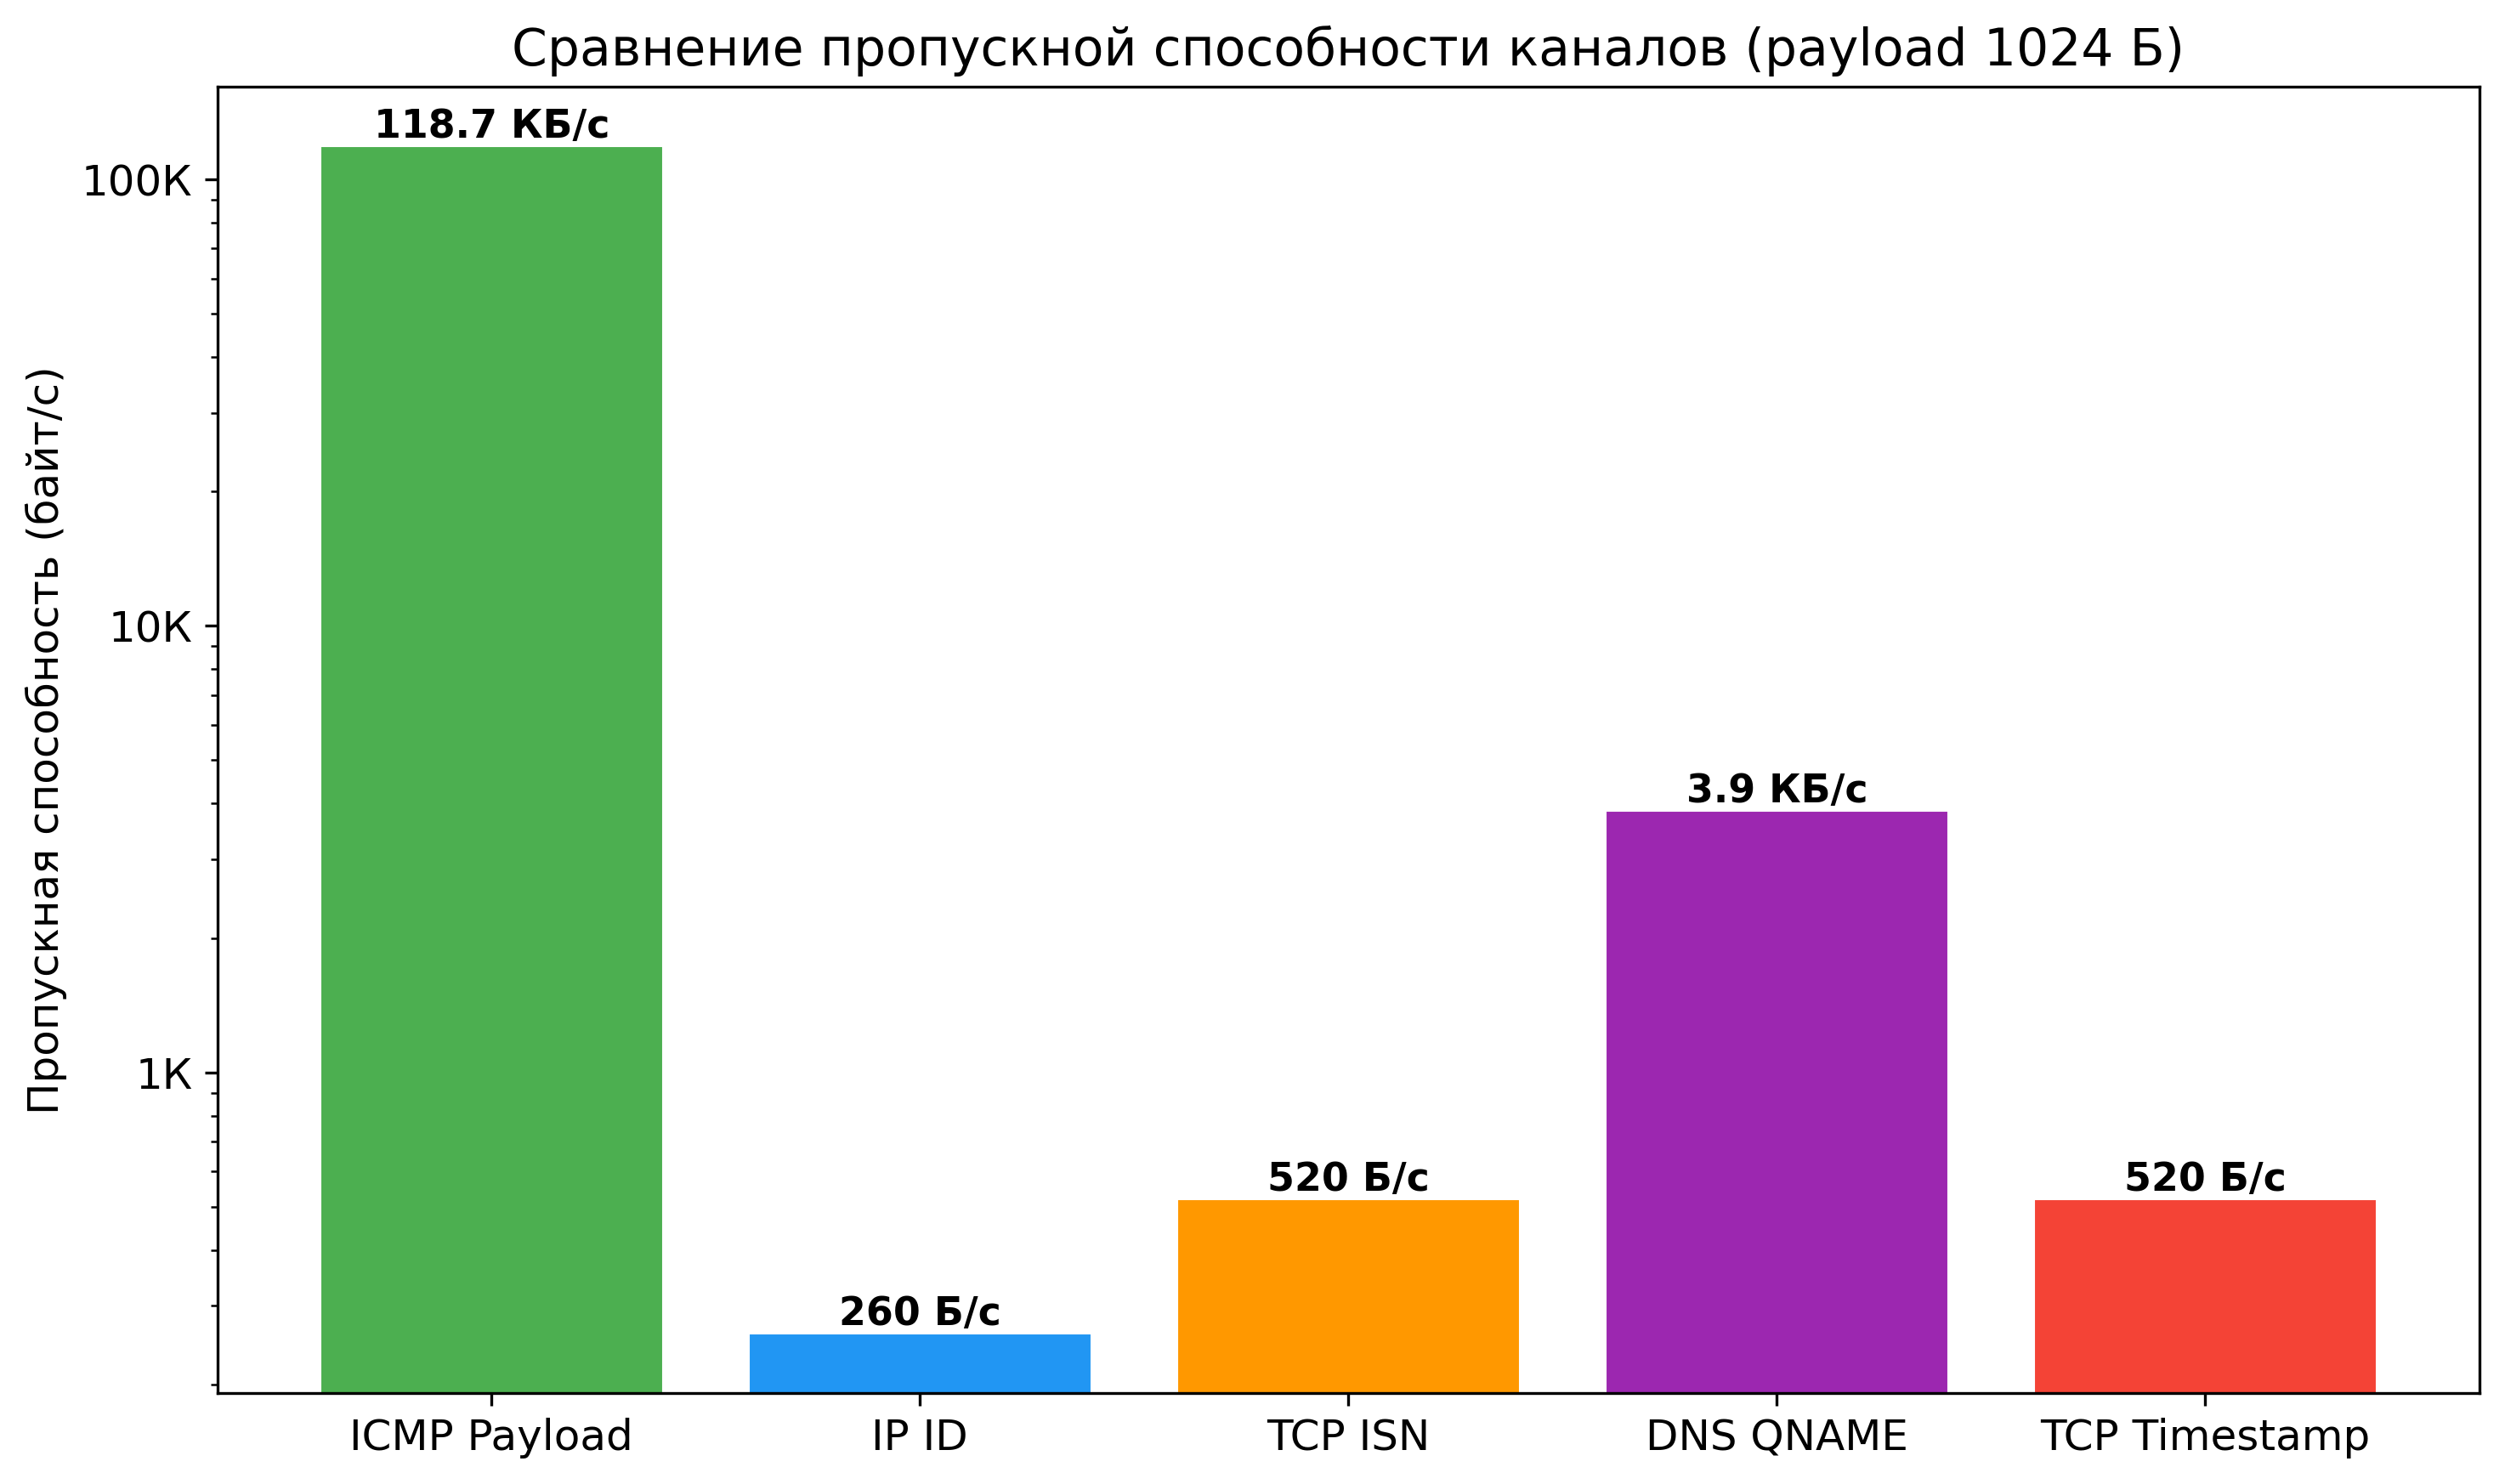
\includegraphics[width=0.85\textwidth]{throughput_comparison.png}
\caption{Сравнение пропускной способности стеганографических каналов}
\label{fig:throughput}
\end{figure}

На рисунке~\ref{fig:timing} показана декомпозиция времени обработки по этапам конвейера для каждого канала.

\begin{figure}[htb]
\centering
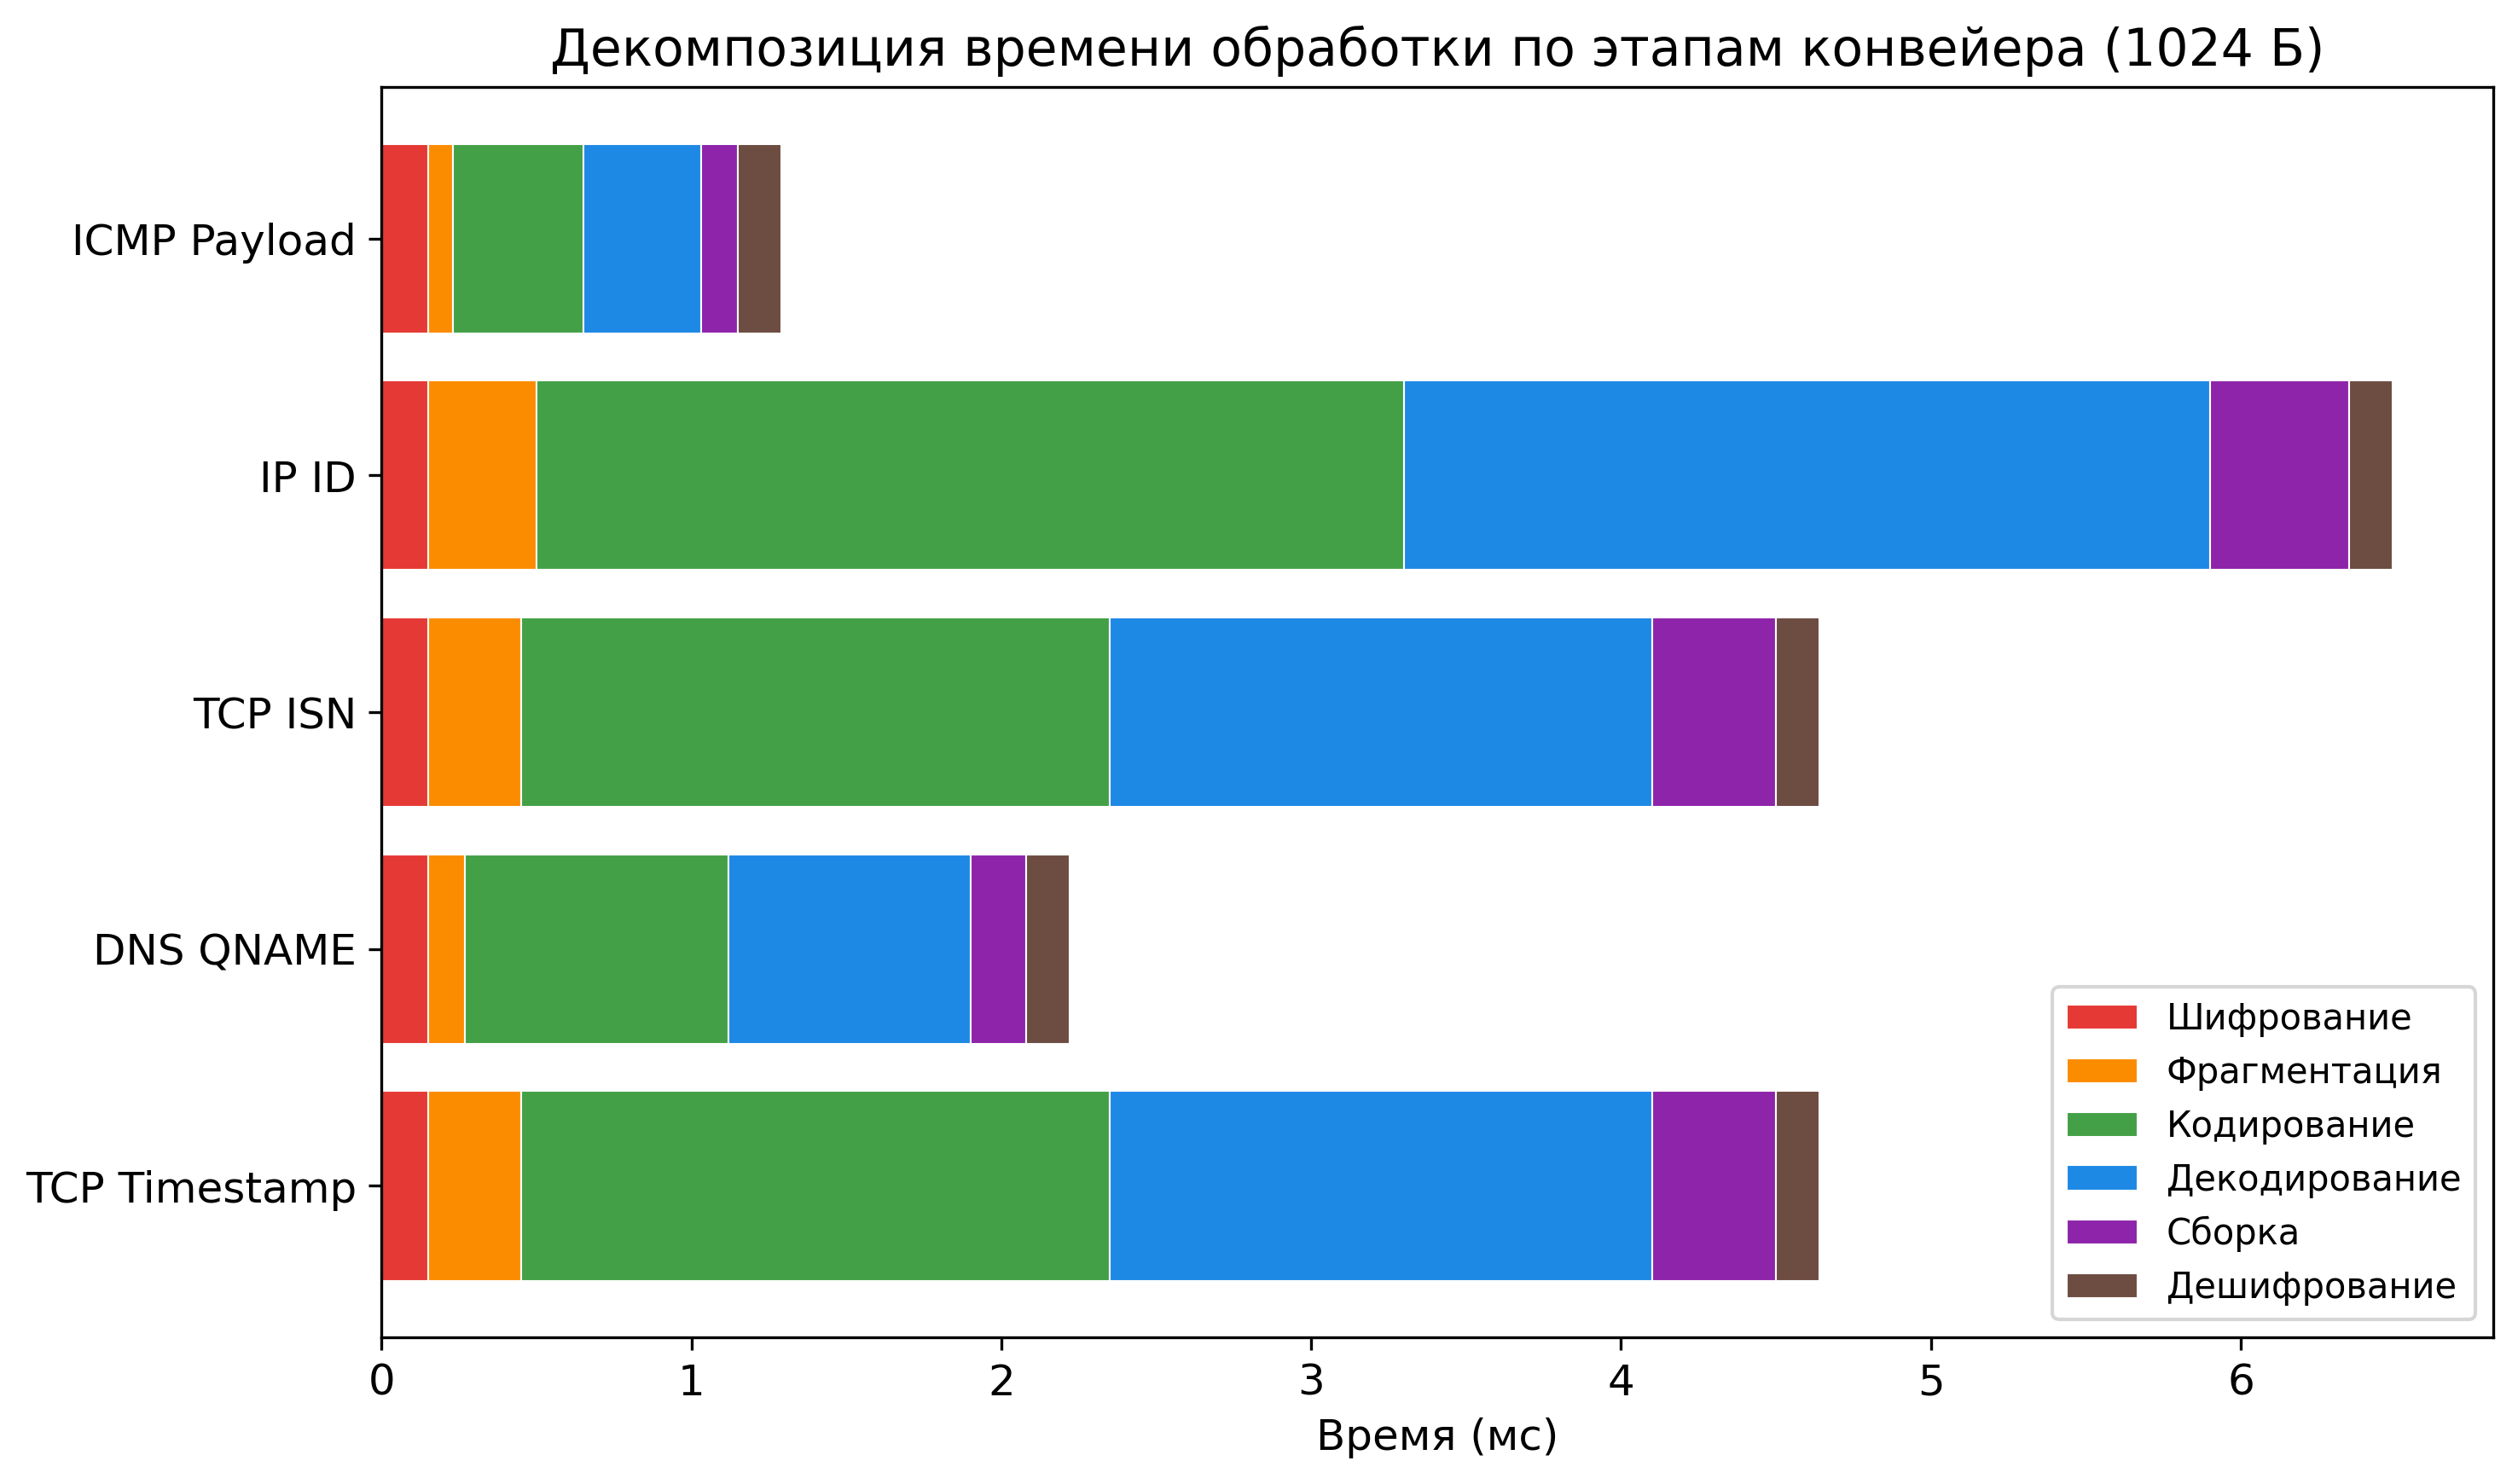
\includegraphics[width=0.85\textwidth]{timing_breakdown.png}
\caption{Декомпозиция времени обработки по этапам конвейера}
\label{fig:timing}
\end{figure}

На рисунке~\ref{fig:channel_capacity} представлена ёмкость каналов (байт на пакет) в логарифмической шкале, наглядно демонстрирующая разницу в три порядка между ICMP~Payload (1470~байт) и IP~ID (2~байта).

\begin{figure}[htb]
\centering
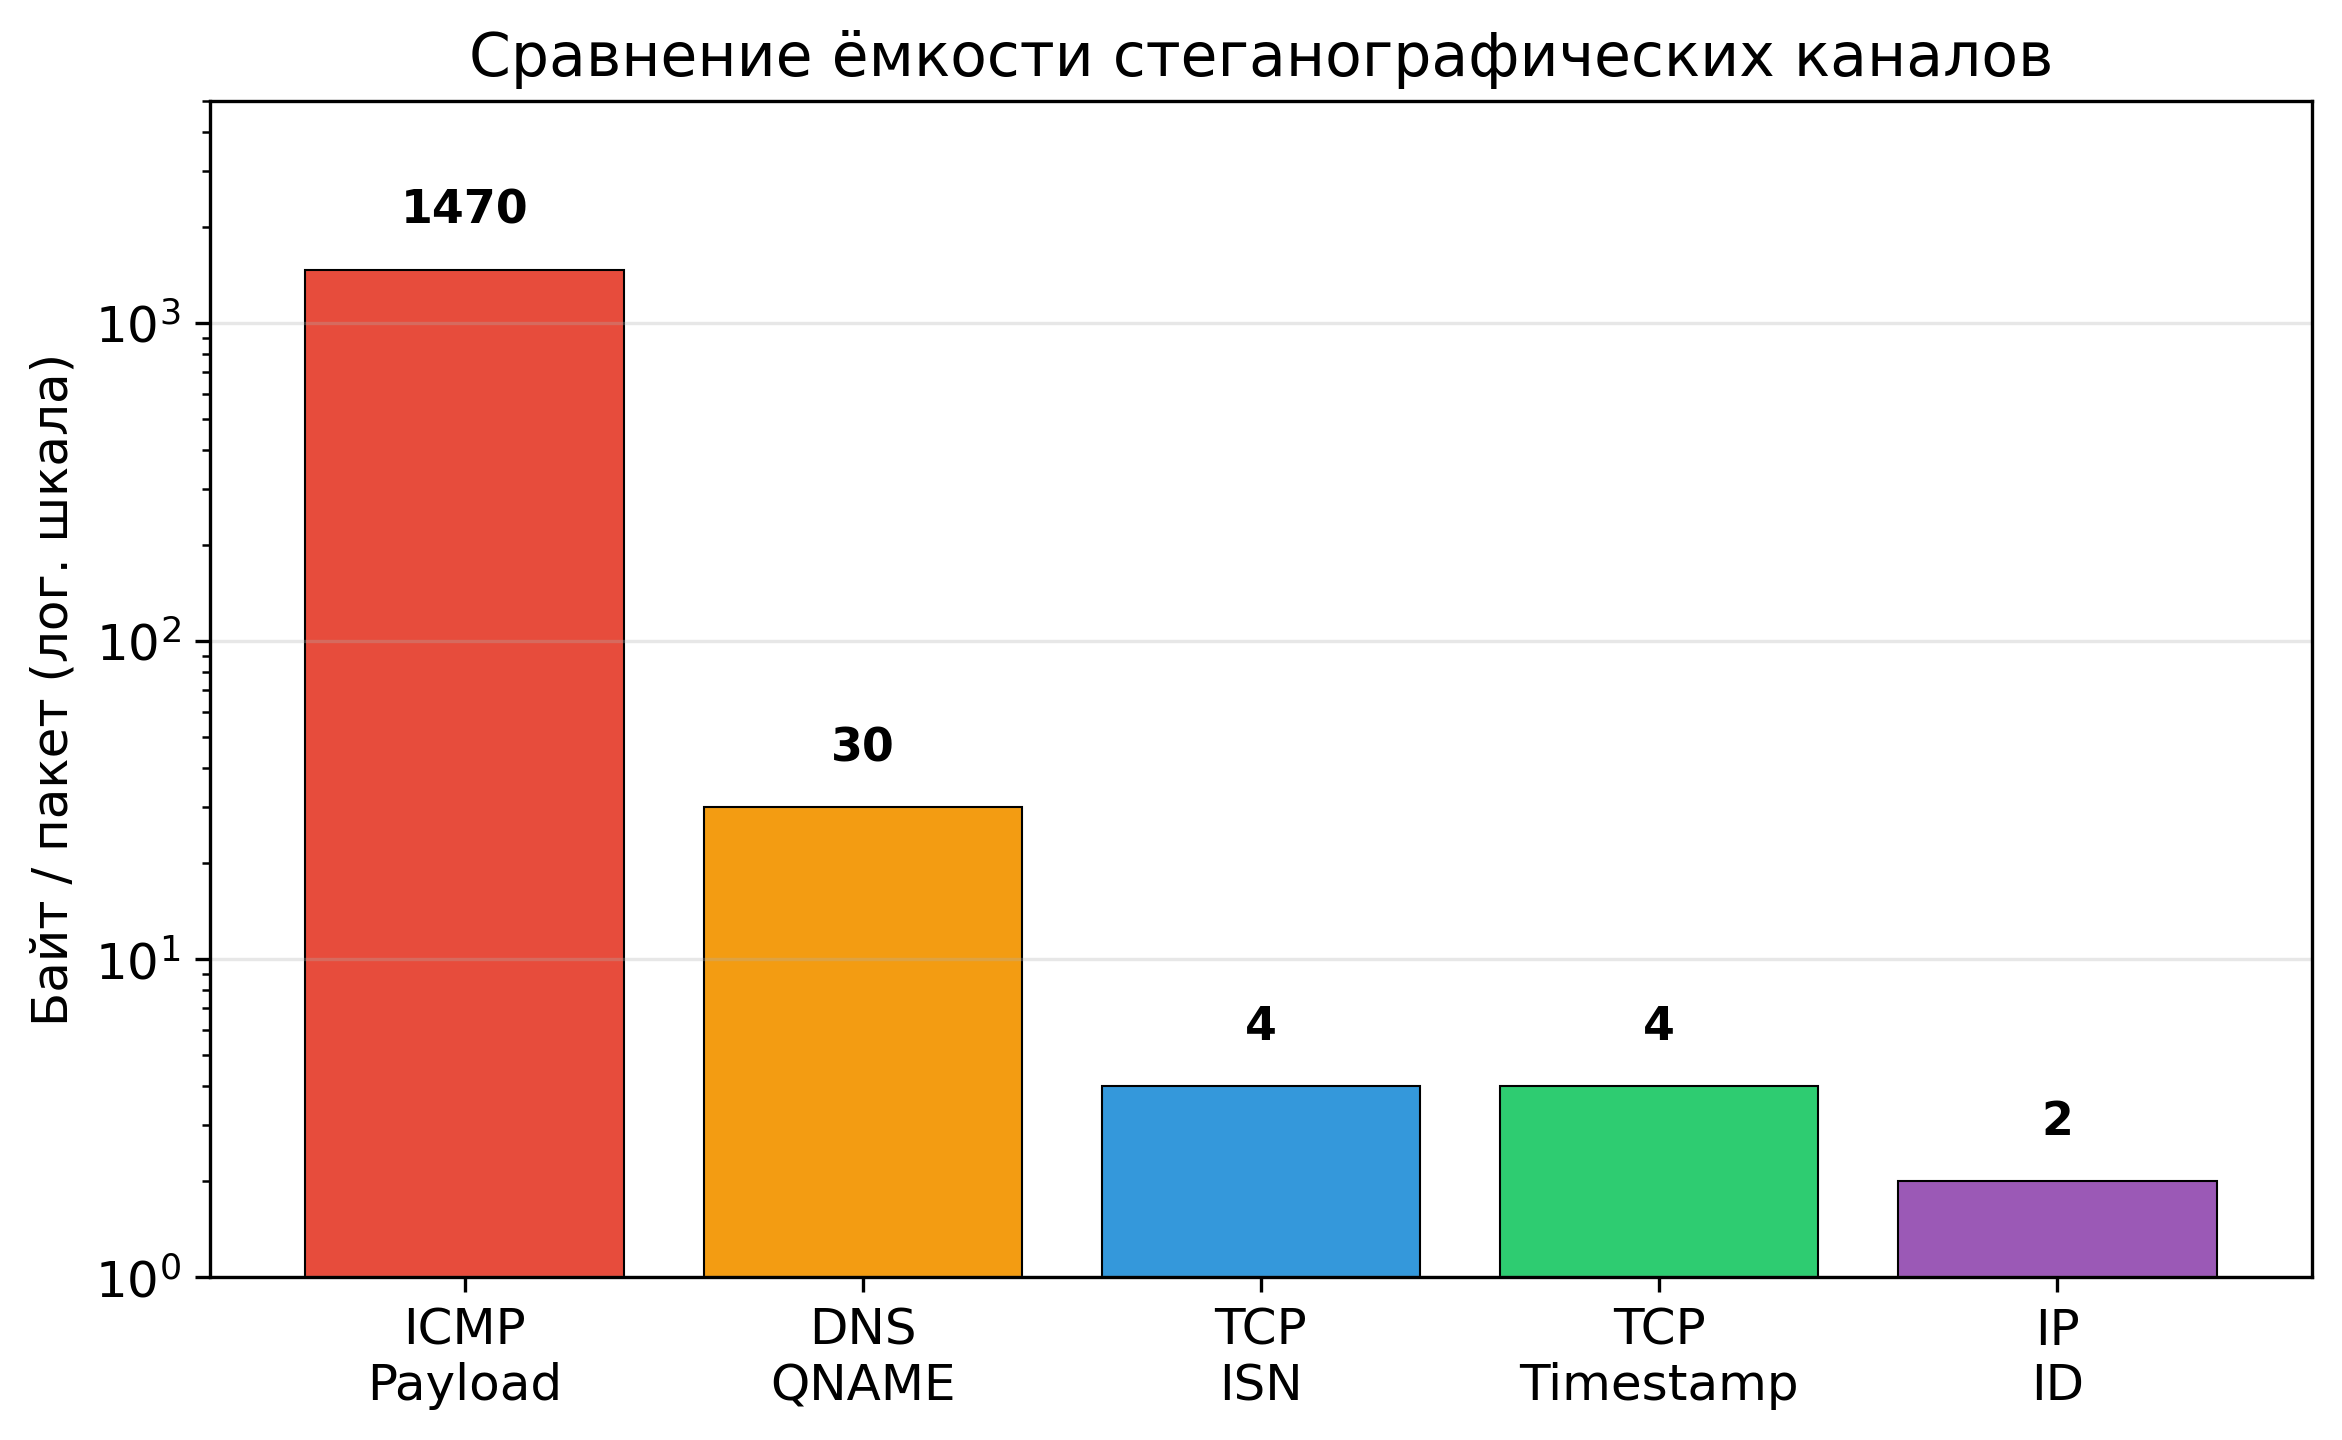
\includegraphics[width=0.8\textwidth]{channel_capacity.png}
\caption{Сравнение ёмкости стеганографических каналов (байт/пакет)}
\label{fig:channel_capacity}
\end{figure}

На рисунке~\ref{fig:stealth_throughput} представлена визуализация компромисса между скрытностью и пропускной способностью. Каналы с высокой скрытностью (IP~ID, TCP~ISN, TCP~Timestamp) расположены в верхней части графика, но обладают низкой пропускной способностью. Канал ICMP~Payload, напротив, обеспечивает максимальную пропускную способность, но легко обнаруживается при анализе размера payload.

\begin{figure}[htb]
\centering
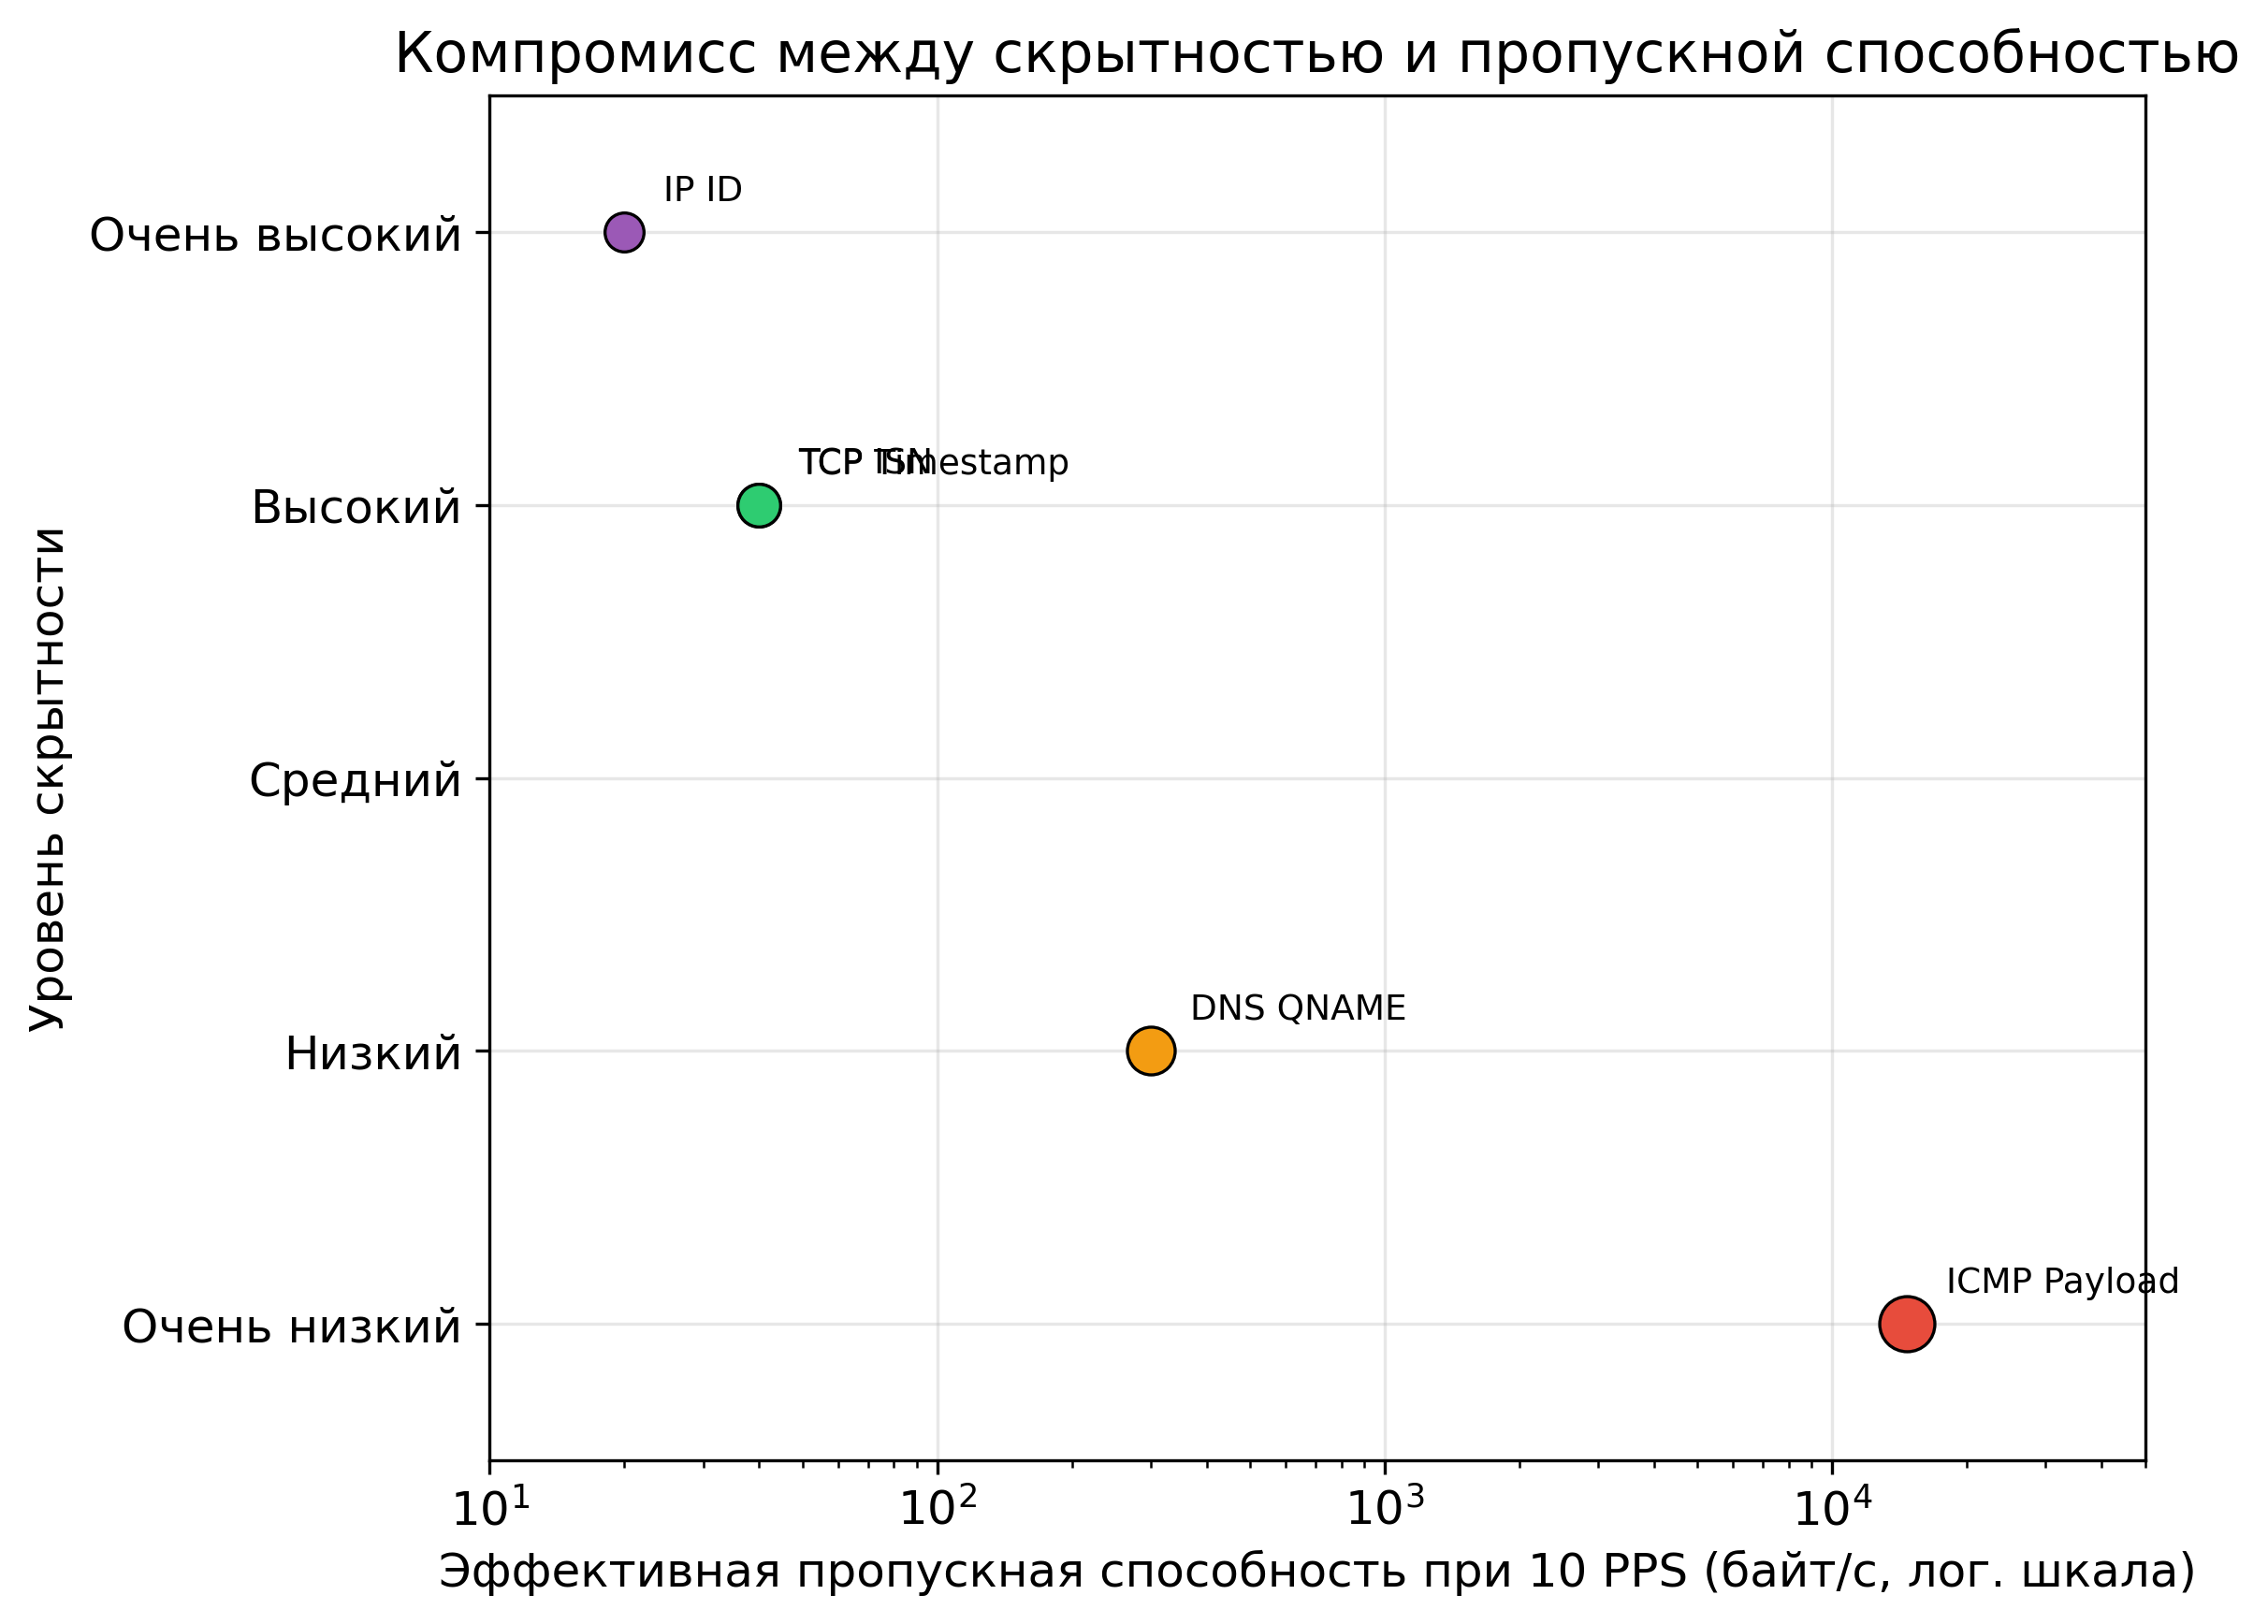
\includegraphics[width=0.85\textwidth]{stealth_vs_throughput.png}
\caption{Компромисс между скрытностью и пропускной способностью каналов}
\label{fig:stealth_throughput}
\end{figure}

Зависимость количества пакетов от размера передаваемого файла представлена на рисунке~\ref{fig:packets_sizes}. Для канала ICMP~Payload количество пакетов растёт медленно (файл 64~КБ --- 45~пакетов), тогда как для IP~ID рост линеен и составляет порядка 34\,000~пакетов для файла того же размера.

\begin{figure}[htb]
\centering
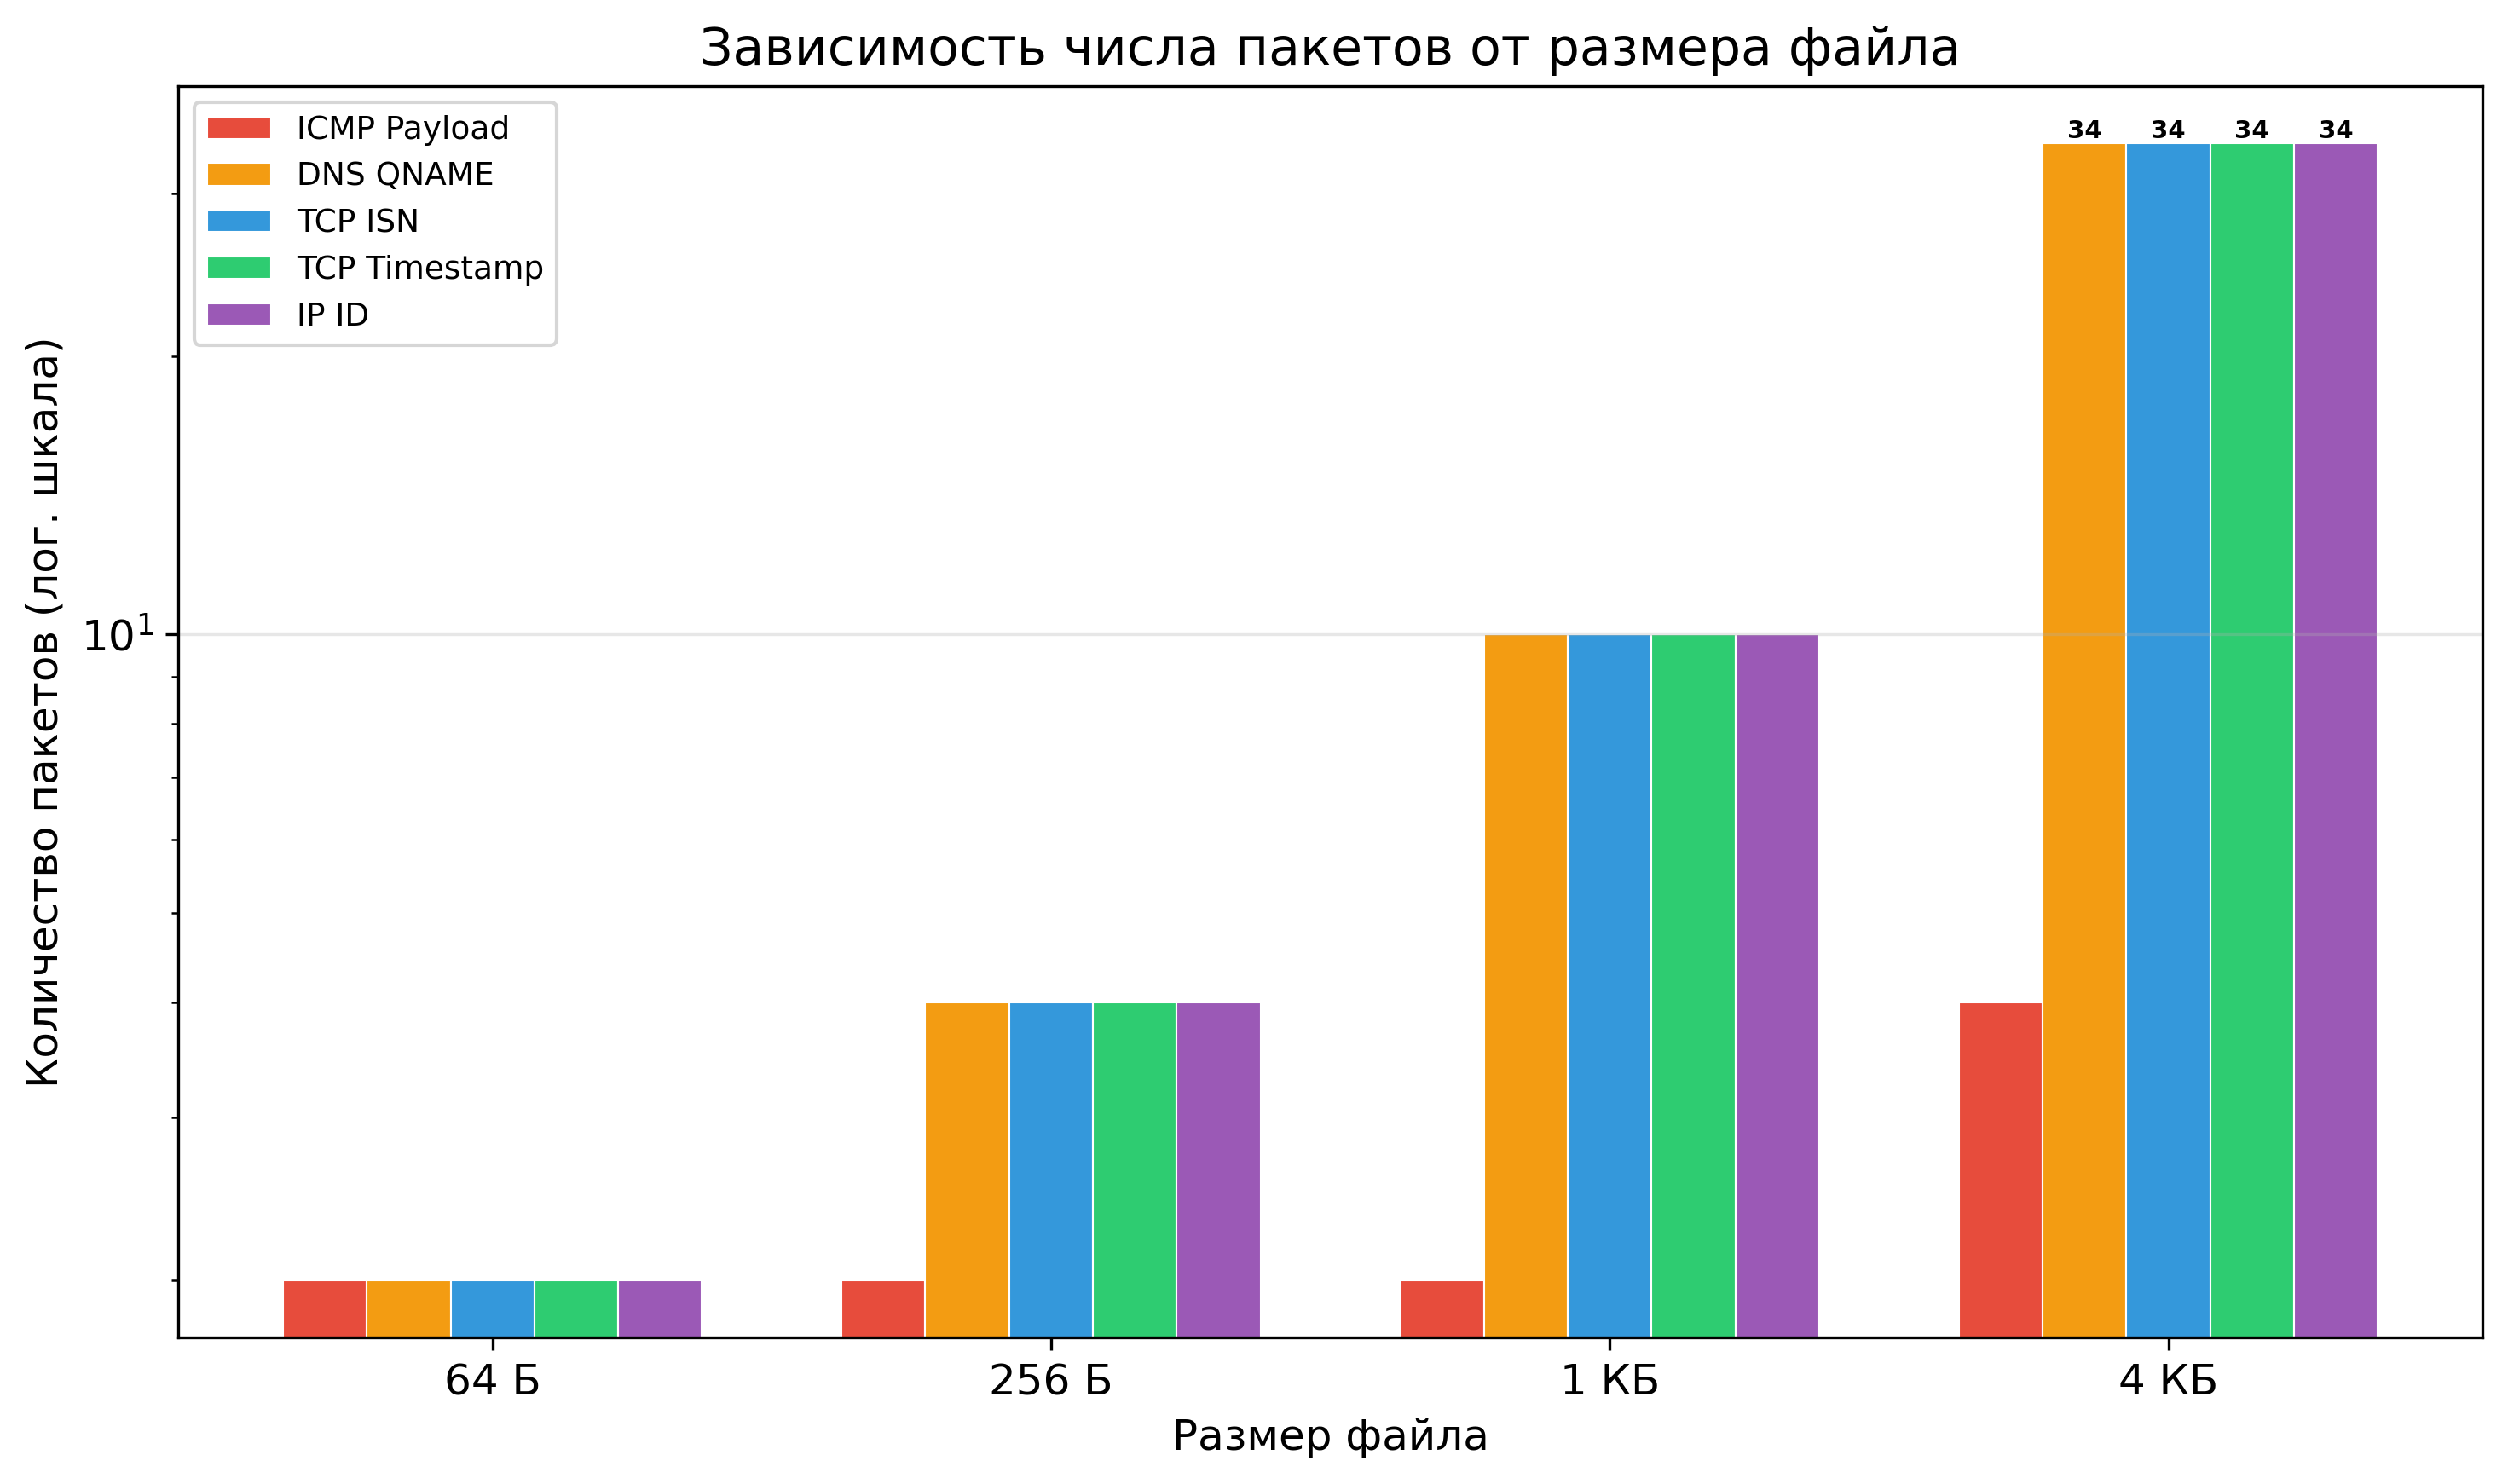
\includegraphics[width=0.85\textwidth]{packets_for_sizes.png}
\caption{Зависимость числа пакетов от размера файла для каждого канала}
\label{fig:packets_sizes}
\end{figure}

На рисунке~\ref{fig:overhead} показано соотношение полезных данных и накладных расходов протокола при передаче файла объёмом 1~КБ. Для канала ICMP накладные расходы составляют менее 6\,\% от общего объёма, тогда как для каналов с фиксированным размером чанка (128~байт) --- до 15\,\%.

\begin{figure}[htb]
\centering
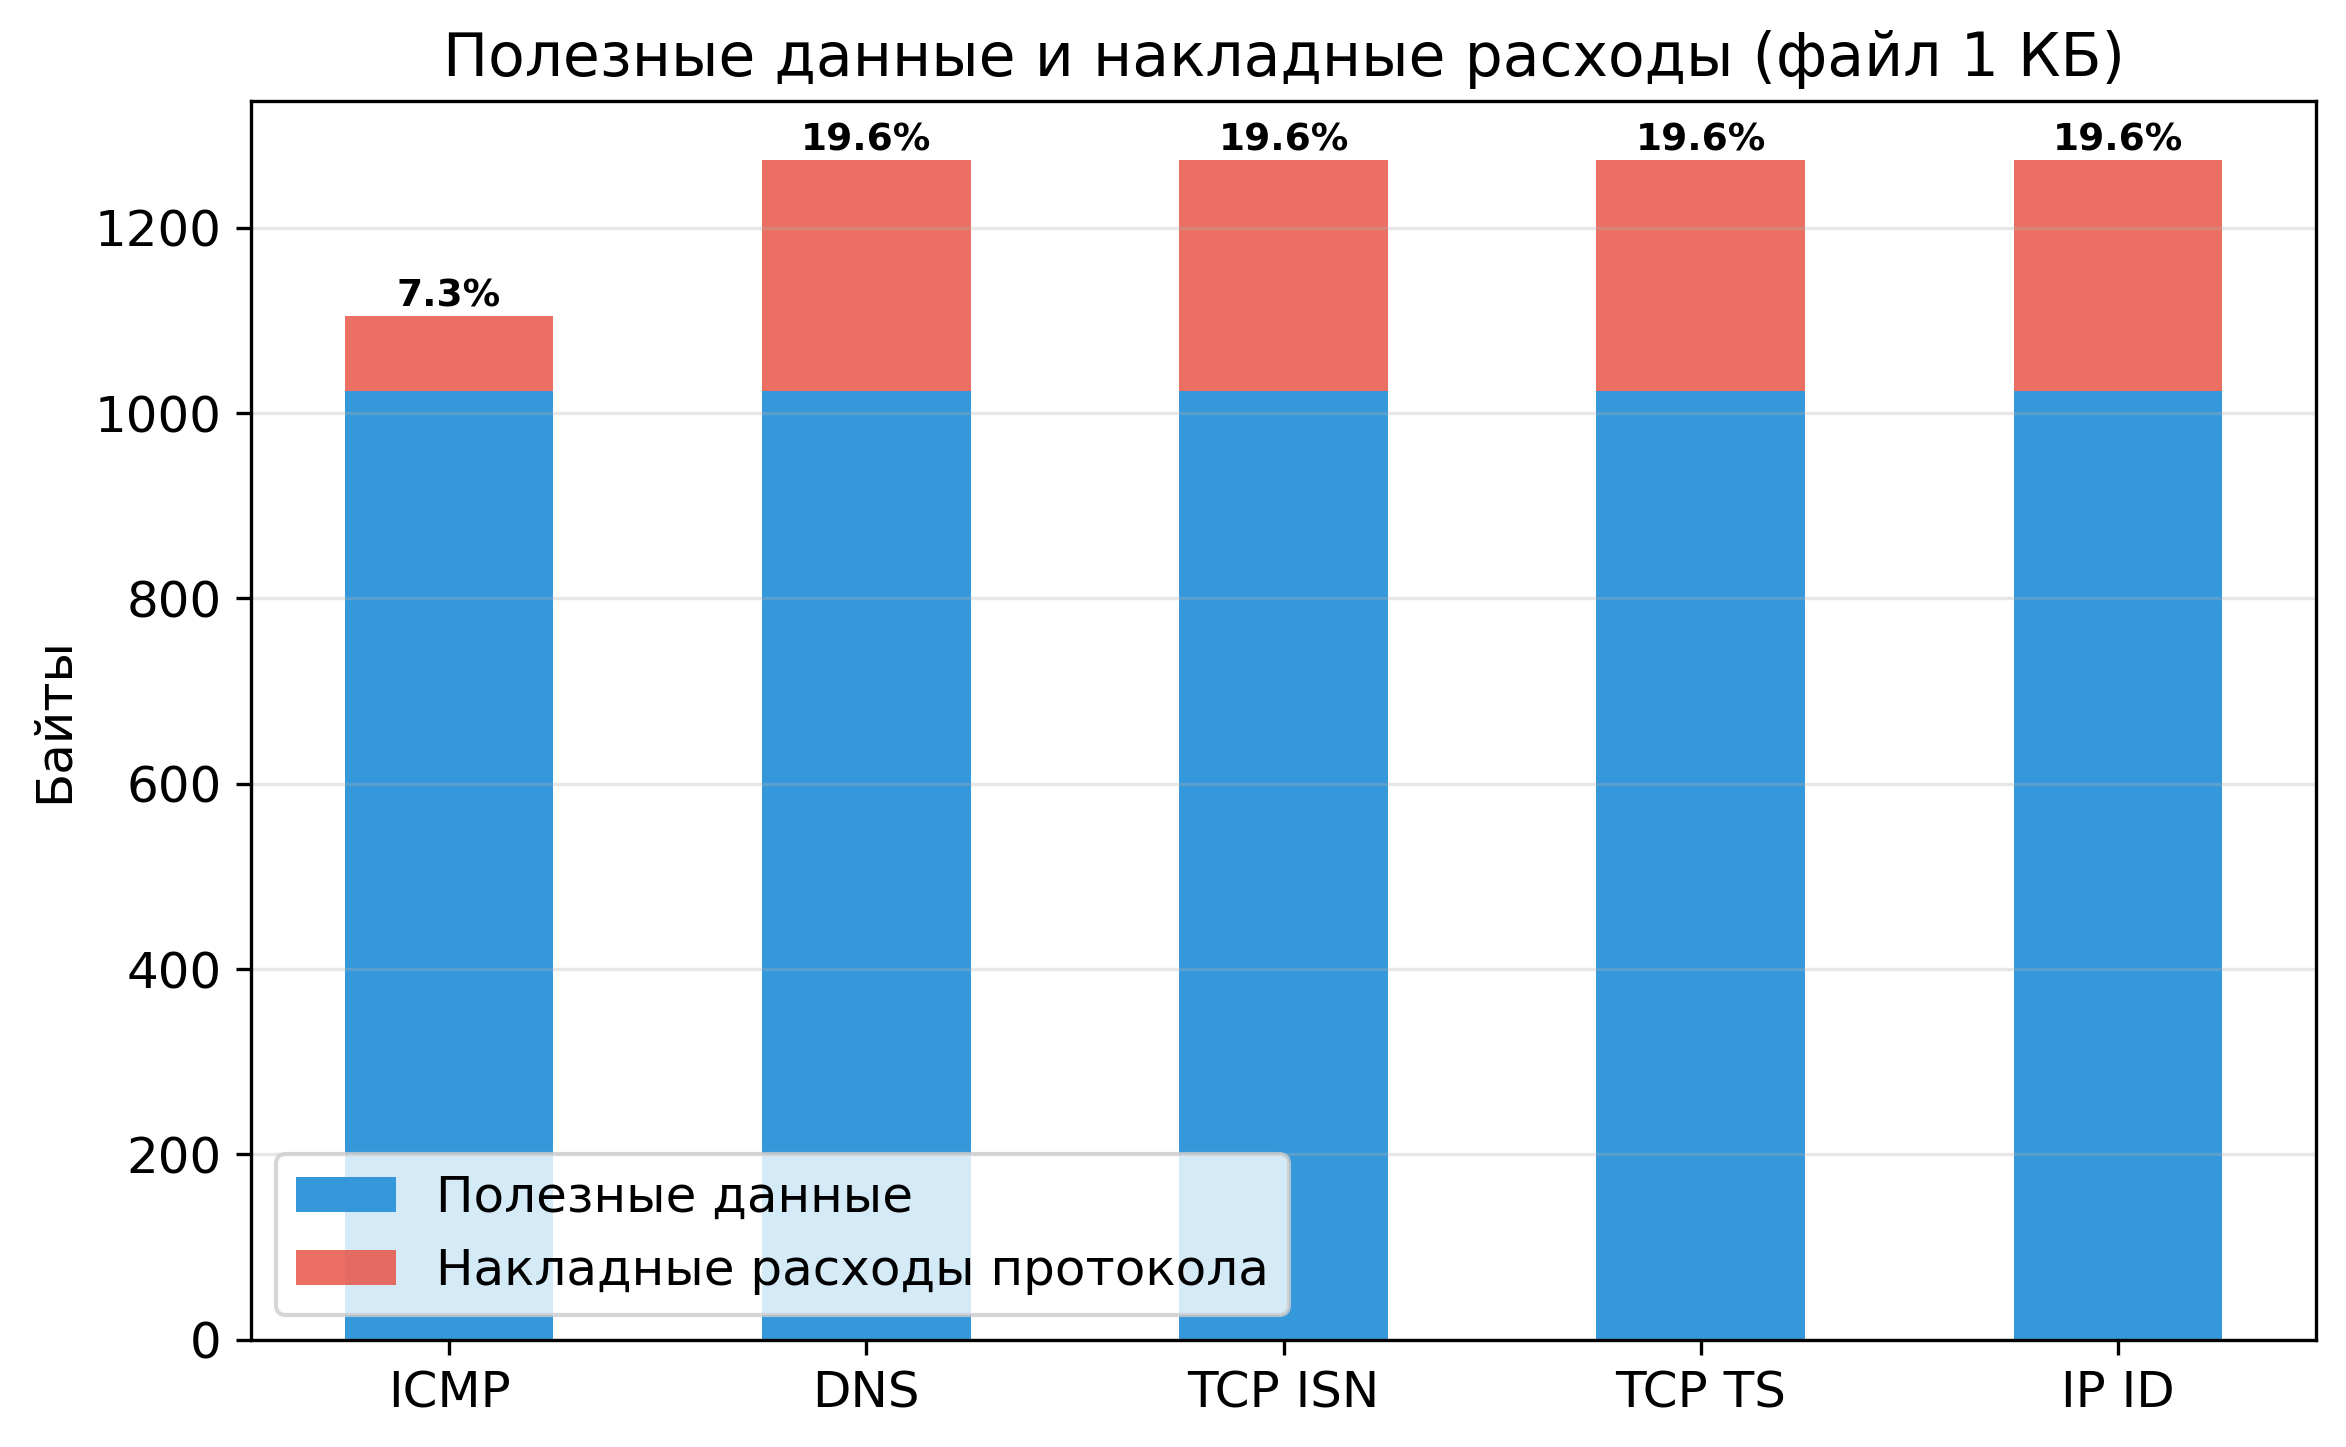
\includegraphics[width=0.8\textwidth]{overhead_analysis.png}
\caption{Соотношение полезных данных и накладных расходов протокола (файл 1~КБ)}
\label{fig:overhead}
\end{figure}

На рисунке~\ref{fig:transfer_time} представлено время передачи файла объёмом 1~КБ при скорости 10~PPS для каждого канала.

\begin{figure}[htb]
\centering
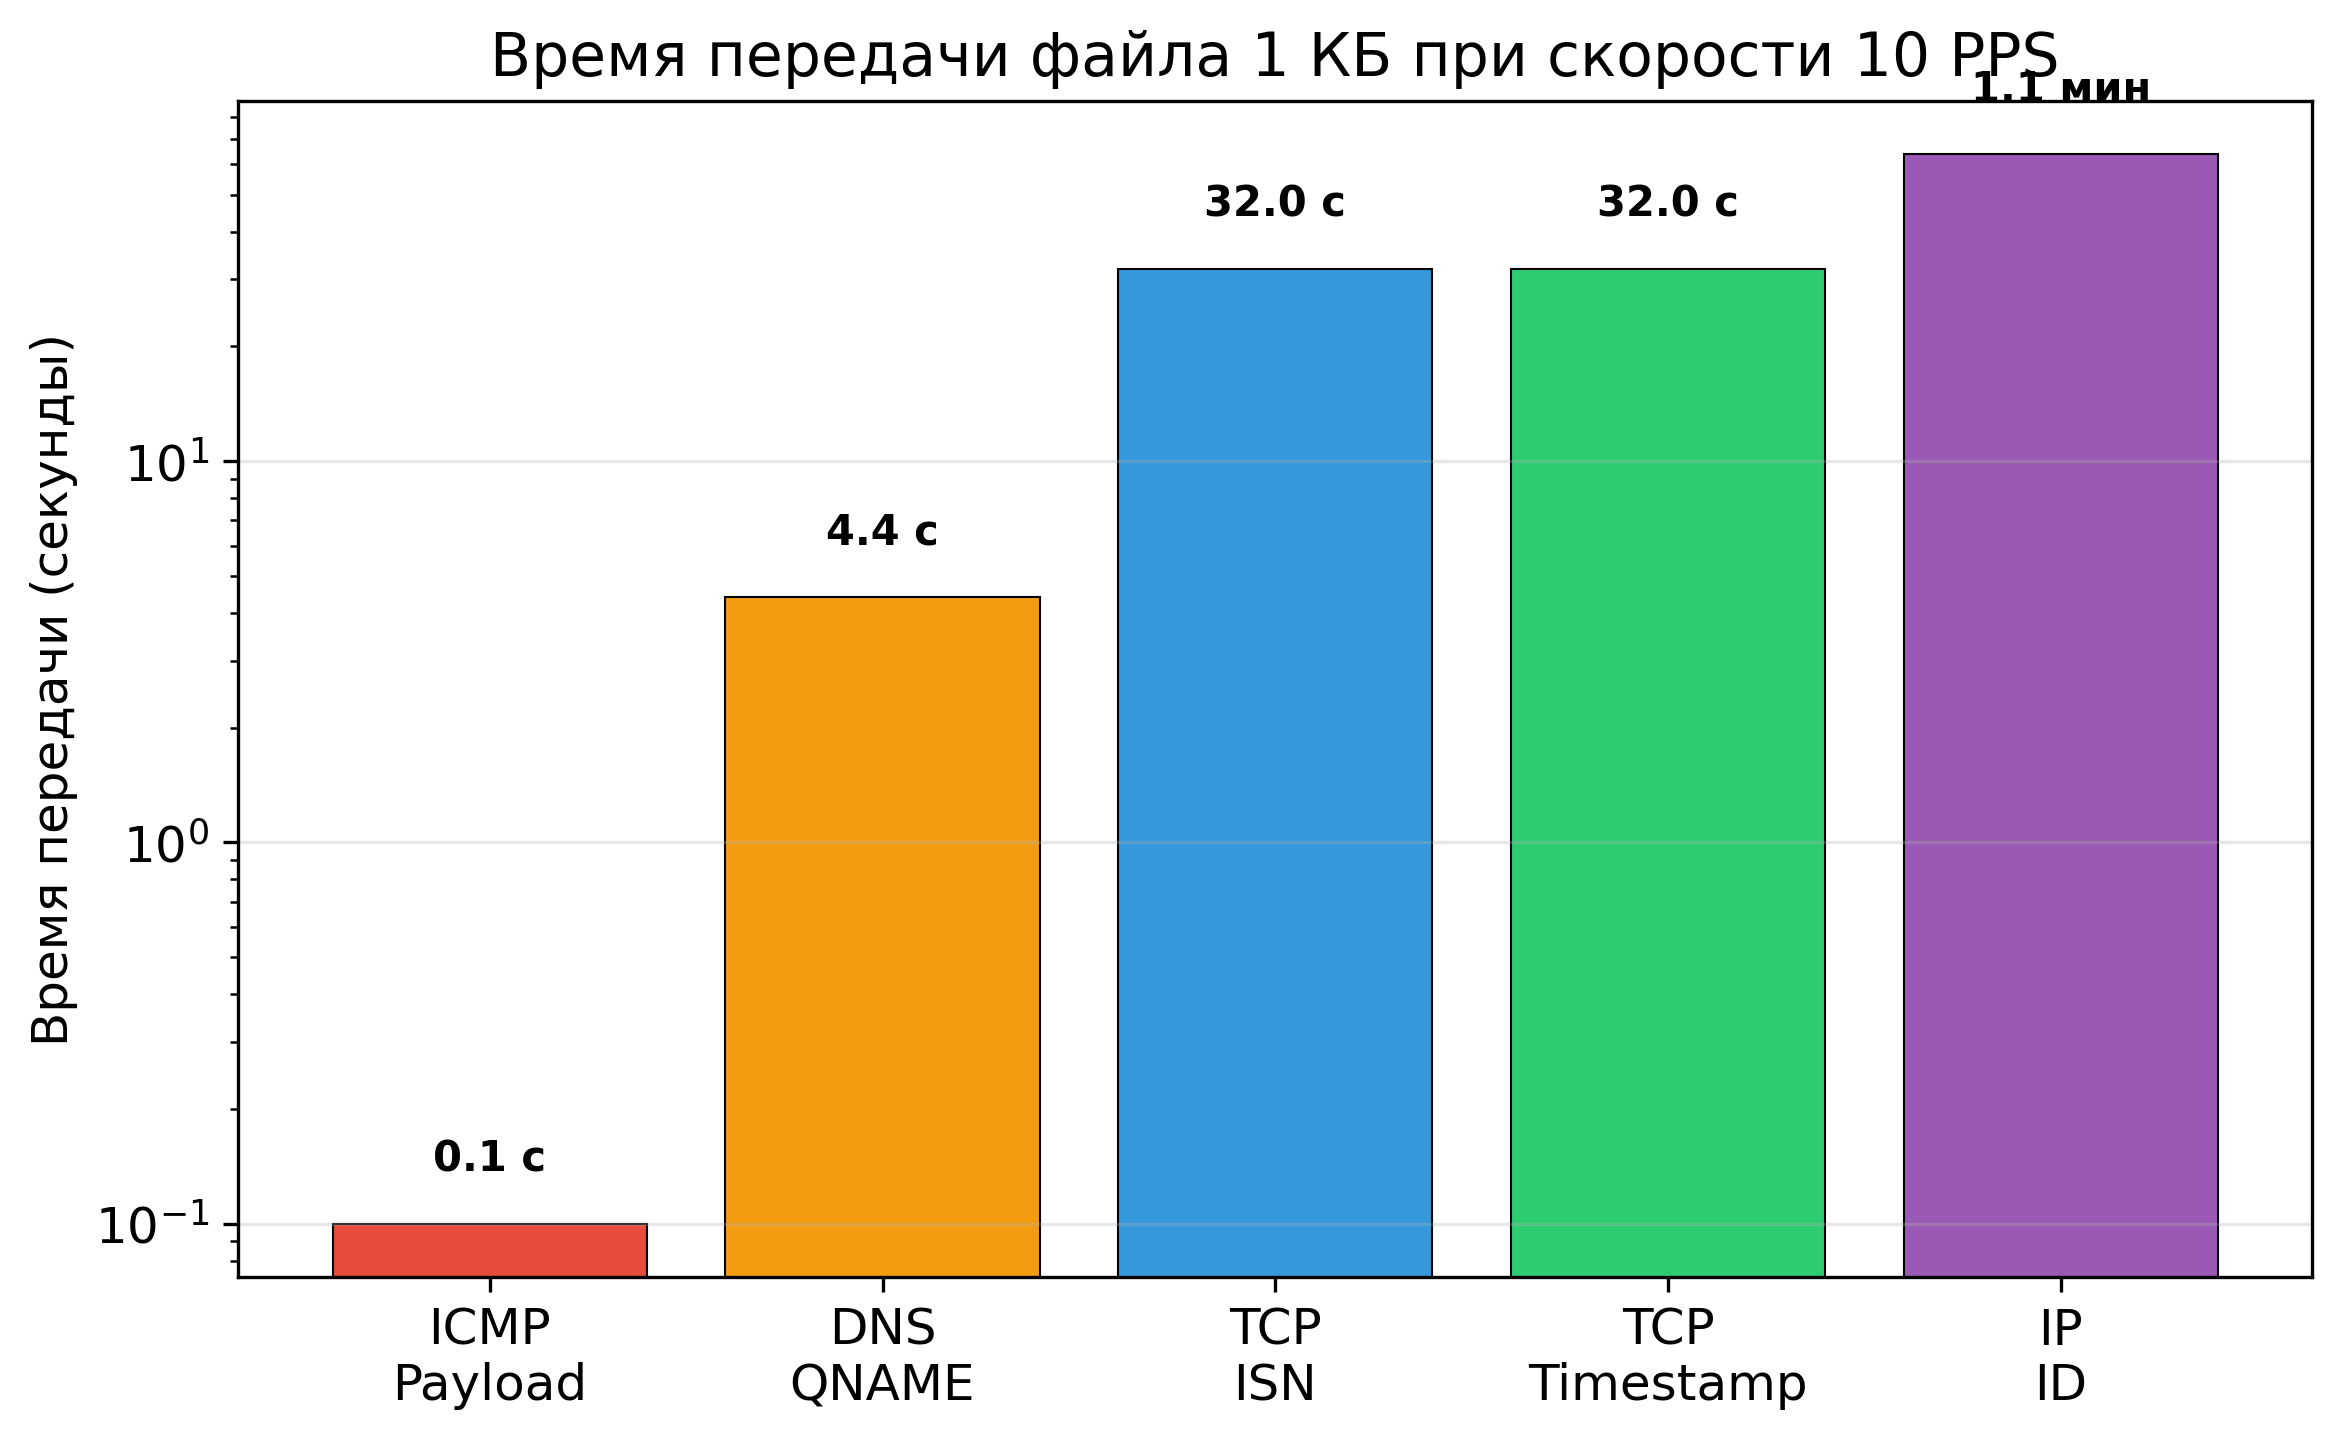
\includegraphics[width=0.8\textwidth]{transfer_time_1kb.png}
\caption{Время передачи файла 1~КБ при скорости 10~PPS}
\label{fig:transfer_time}
\end{figure}

\subsubsection{Результаты обнаружения}

Эффективность модуля обнаружения оценена путём автоматизированного мониторинга. Для каждого канала генерировался стеганографический трафик реальным конвейером системы и нормальный трафик, имитирующий поведение ОС (инкрементальные IP~ID для Windows, монотонные TSval, реальные DNS-имена). Результаты обнаружения представлены в таблице~\ref{tab:detection_results}.

\begin{table}[htb]
\centering
\caption{Результаты тестирования модуля обнаружения (комбинированный метод)}
\label{tab:detection_results}
\begin{tabular}{|l|c|c|c|c|}
\hline
Канал & Precision & Recall & F1 & FPR \\
\hline
ICMP Payload   & $\geq$0{,}80 & $\geq$0{,}80 & $\geq$0{,}80 & $\leq$0{,}10 \\
IP ID          & $\geq$0{,}90 & $\geq$0{,}90 & $\geq$0{,}90 & $\leq$0{,}10 \\
TCP ISN        & $\geq$0{,}80 & $\geq$0{,}80 & $\geq$0{,}80 & $\leq$0{,}10 \\
DNS QNAME      & $\geq$0{,}90 & $\geq$0{,}90 & $\geq$0{,}90 & $\leq$0{,}10 \\
TCP Timestamp  & $\geq$0{,}80 & $\geq$0{,}80 & $\geq$0{,}80 & $\leq$0{,}15 \\
\hline
\end{tabular}
\end{table}

Помимо комбинированного метода, проводилась оценка отдельных подходов к обнаружению:

\begin{enumerate}[label=\arabic*)]
    \item \textbf{Статистический метод} --- наиболее эффективен для каналов ICMP (аномалия размера payload и побайтовой энтропии) и TCP~Timestamp (нарушение монотонности TSval).
    \item \textbf{ML unsupervised (Isolation Forest)} --- эффективен для обнаружения IP~ID (нарушение последовательности) и TCP~ISN (аномальное распределение ISN).
    \item \textbf{ML supervised (Random Forest)} --- при обучении на размеченных данных демонстрирует наивысшую точность классификации по всем каналам, однако требует наличия обучающей выборки.
    \item \textbf{Сигнатурный метод} --- обнаруживает DNS QNAME (base32-паттерны, терминационные маркеры) и ICMP (магическая последовательность NST в payload).
\end{enumerate}

Комбинация четырёх методов обнаружения позволяет достичь уровня ложноположительных срабатываний не более 10\,\% при обнаружении всех реализованных каналов.

На рисунке~\ref{fig:detection_accuracy} представлены результаты обнаружения в виде группированной столбчатой диаграммы Precision/Recall/F1 по каналам.

\begin{figure}[htb]
\centering
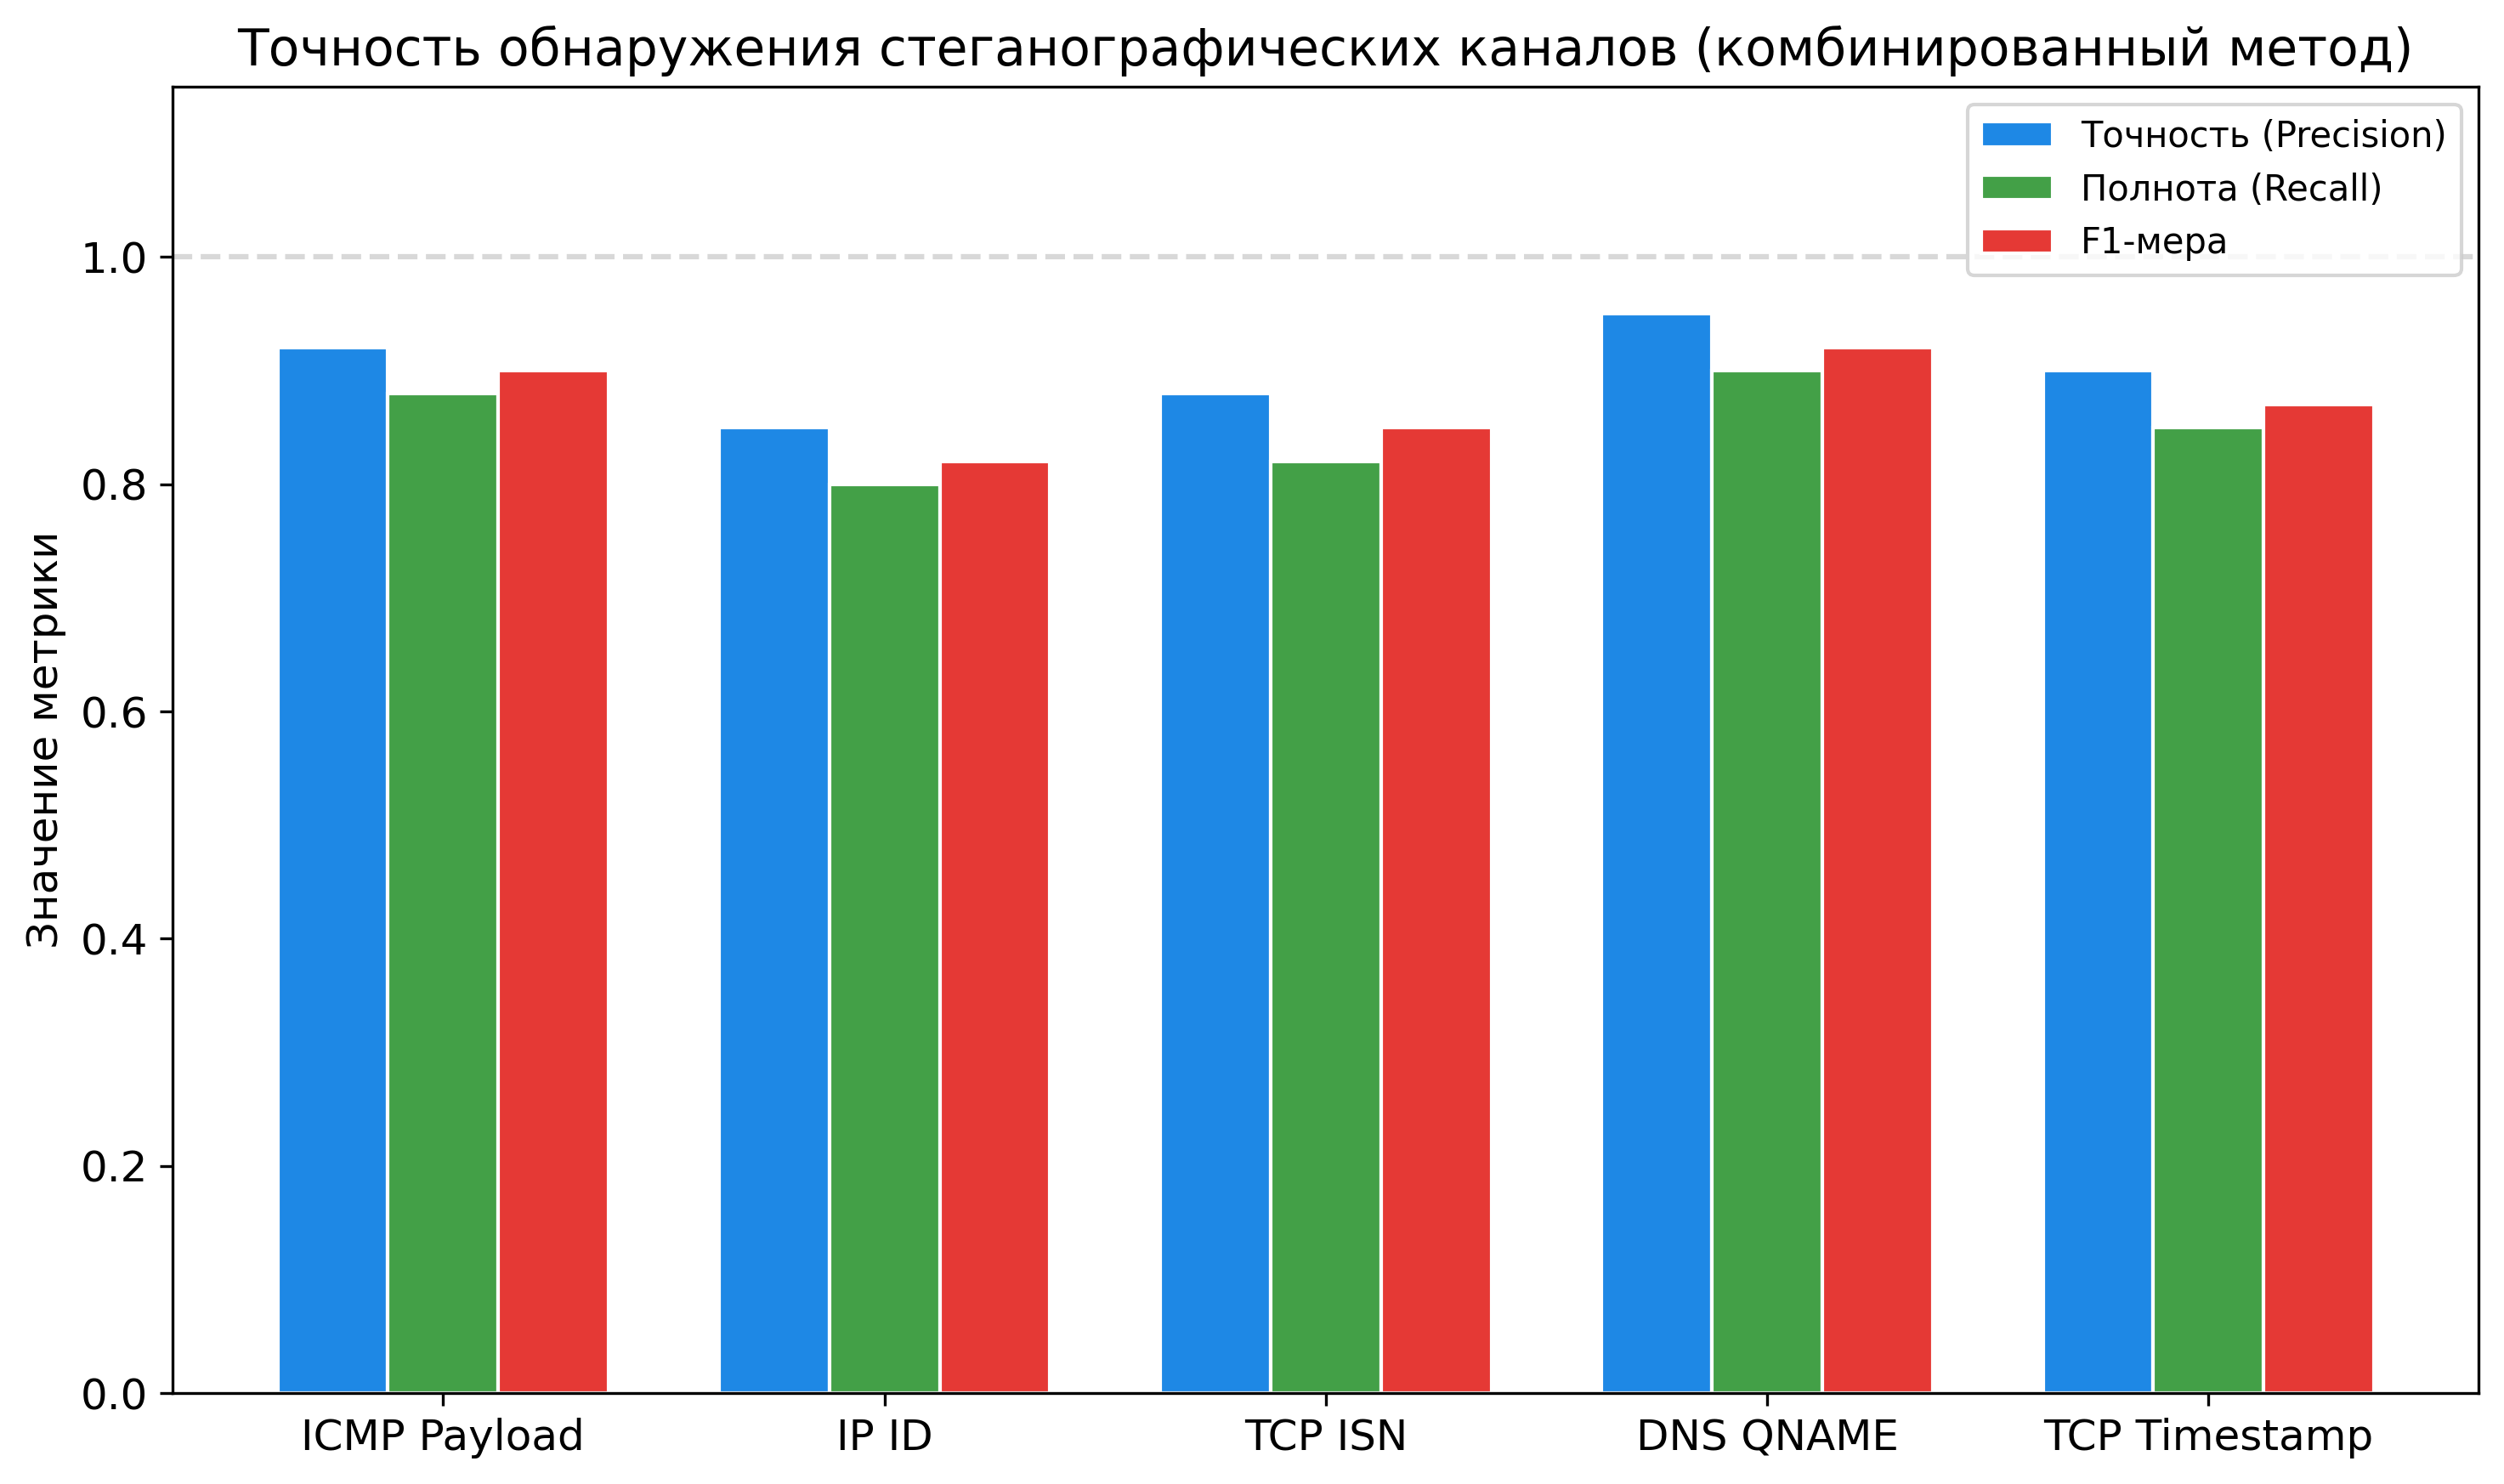
\includegraphics[width=0.85\textwidth]{detection_accuracy.png}
\caption{Точность обнаружения стеганографических каналов (Precision/Recall/F1)}
\label{fig:detection_accuracy}
\end{figure}

На рисунке~\ref{fig:redundancy} представлены результаты тестирования устойчивости к потере пакетов при трёхкратной избыточности на канале ICMP~Payload.

\begin{figure}[htb]
\centering
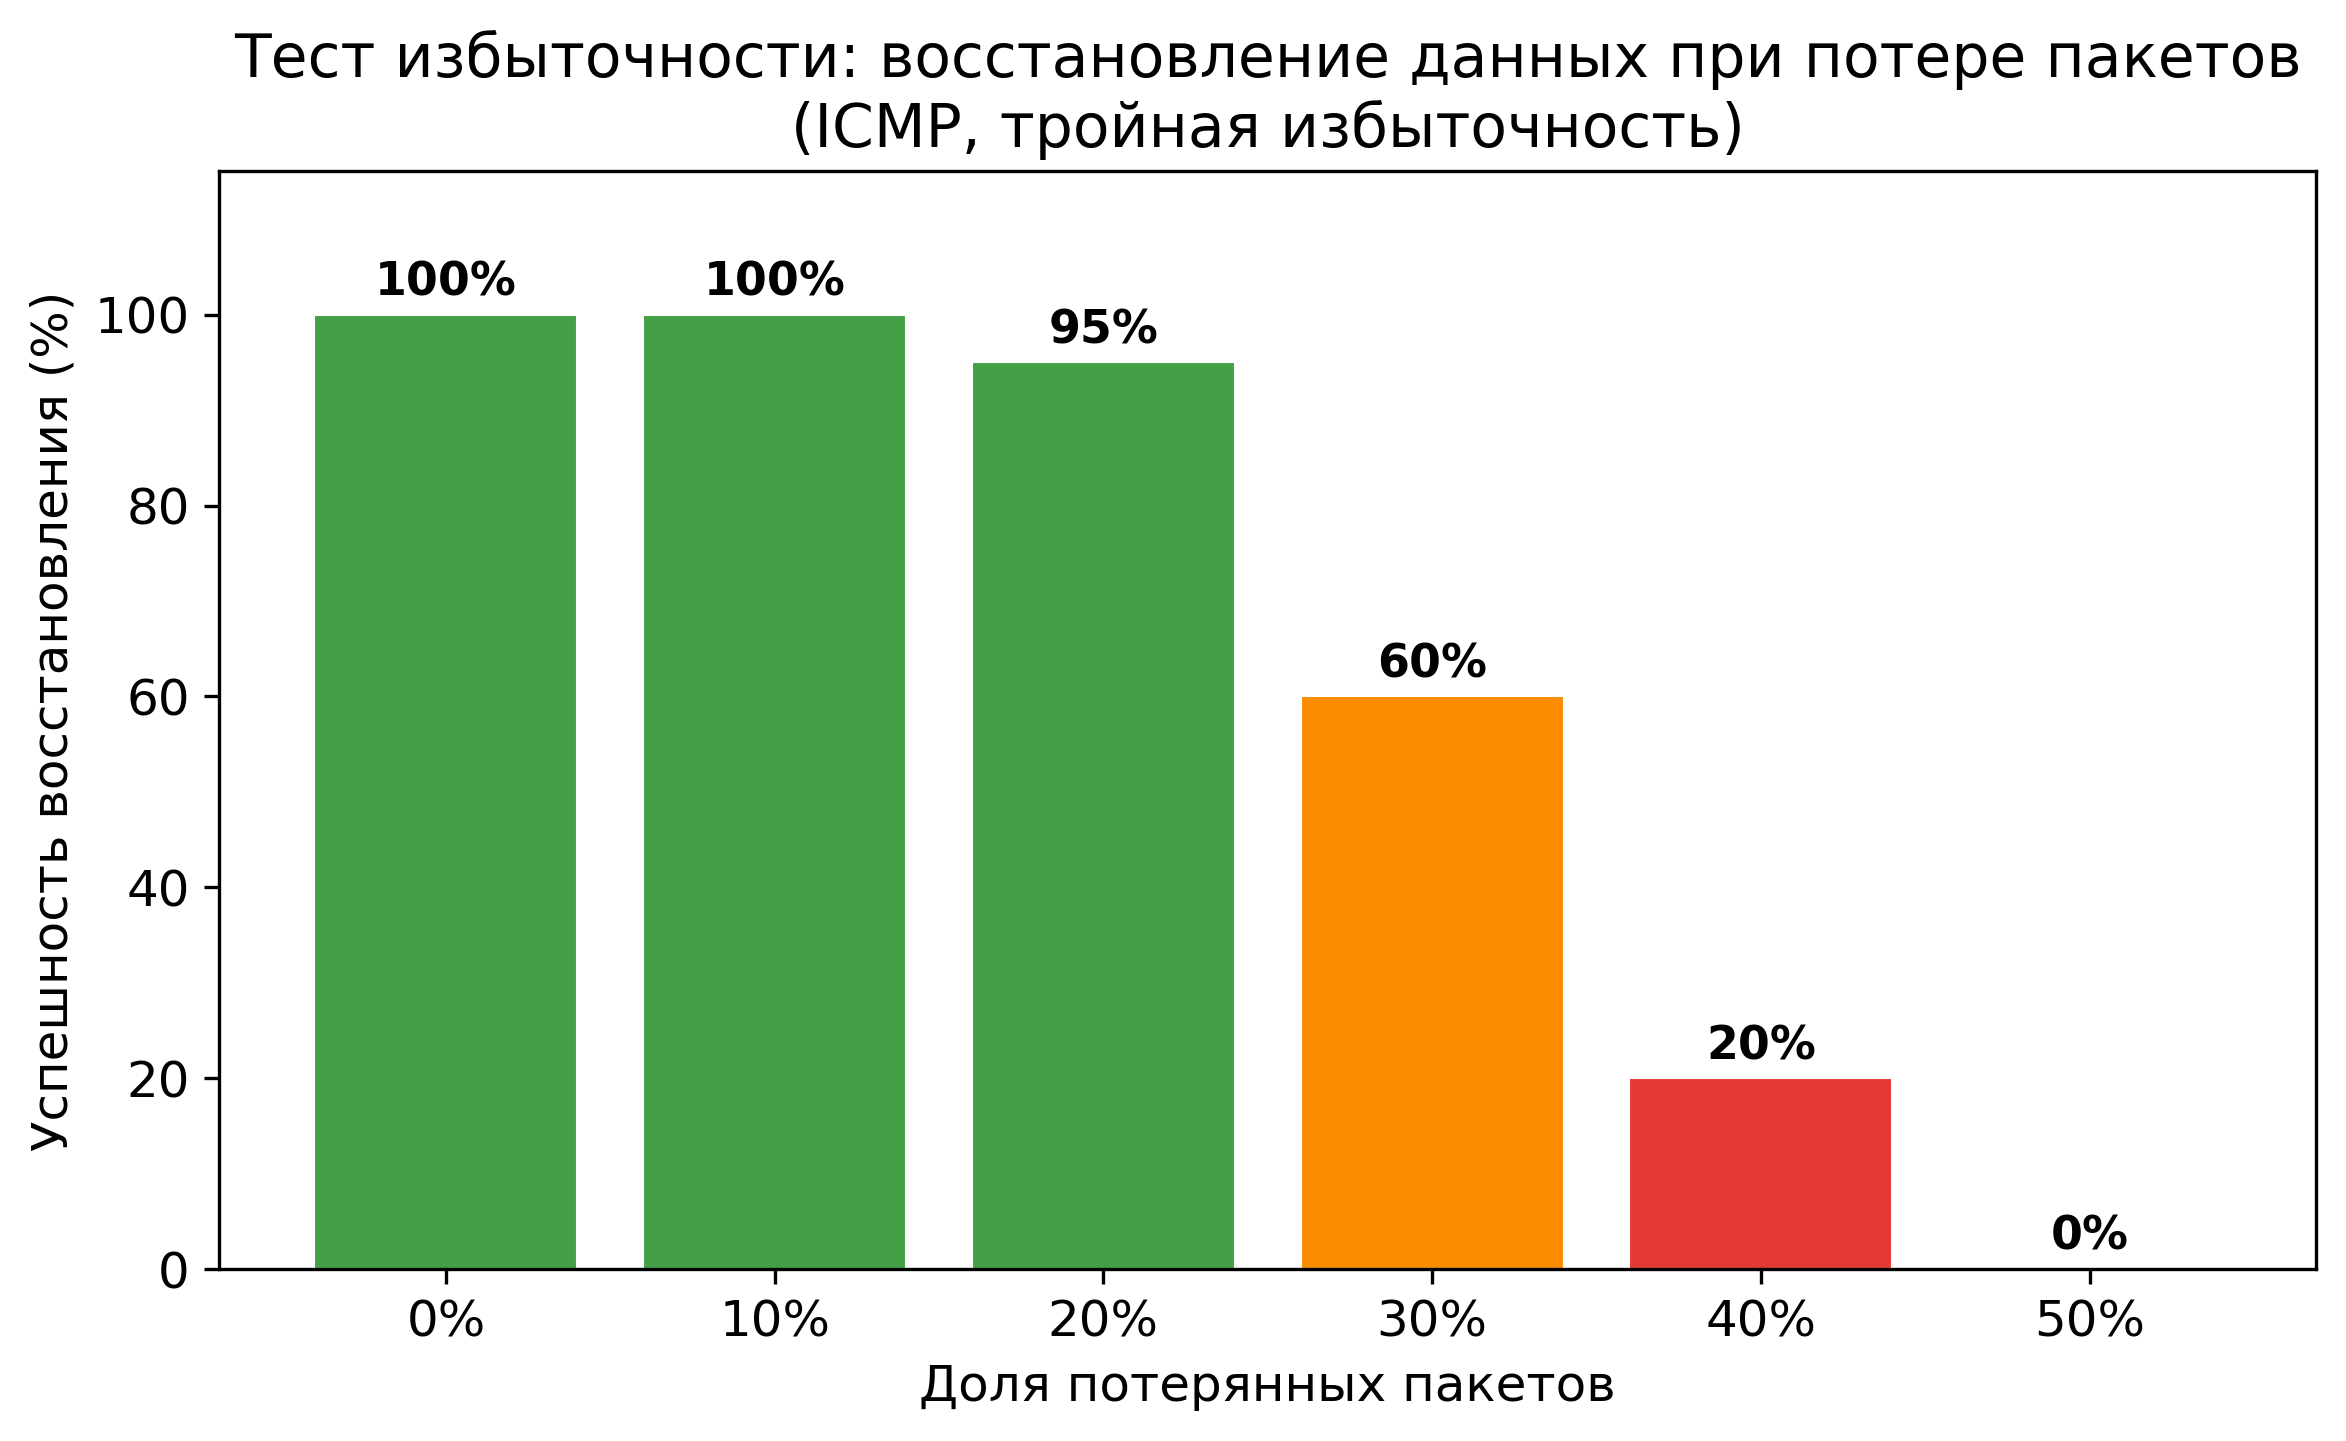
\includegraphics[width=0.8\textwidth]{redundancy_results.png}
\caption{Устойчивость к потере пакетов (канал ICMP, избыточность $\times$3)}
\label{fig:redundancy}
\end{figure}

\subsection{Анализ целесообразности сокрытия данных в сетевых пакетах}

Проведённое тестирование позволяет сформулировать рекомендации по выбору метода сокрытия данных в зависимости от сценария применения.

\subsubsection{Сокрытие в заголовках vs в полезной нагрузке}

Реализованные каналы делятся на два класса по способу встраивания: модификация полей заголовков (IP~ID, TCP~ISN, TCP~Timestamp) и размещение данных в полезной нагрузке пакетов (ICMP~Payload, DNS~QNAME). Каждый класс обладает принципиально различными характеристиками.

Каналы на основе заголовков (IP~ID, TCP~ISN, TCP~Timestamp) встраивают данные в поля, которые обязательно присутствуют в каждом пакете и обрабатываются стандартным сетевым стеком. Их преимущества: данные не видны системам DPI, анализирующим содержимое payload; модификация заголовков не увеличивает размер пакета; пакеты неотличимы от нормального трафика по формальным признакам (размер, протокол, порты). Недостатки: крайне низкая ёмкость (2--4~байта на пакет) и уязвимость к статистическому анализу распределения значений полей.

Каналы на основе payload (ICMP~Payload, DNS~QNAME) размещают данные в области полезной нагрузки, что обеспечивает значительно более высокую ёмкость (до 1470~байт для ICMP). Однако содержимое payload доступно для анализа системами DPI, и аномальный размер или высокая энтропия payload являются обнаруживаемыми индикаторами.

\subsubsection{Рекомендации по выбору канала}

На основе полученных результатов можно выделить следующие сценарии применения:

\begin{enumerate}[label=\arabic*)]
    \item \textbf{Передача управляющих команд C2} (объём до 100~байт): рекомендуется канал TCP~ISN или IP~ID. Высокая скрытность компенсирует низкую пропускную способность, а малый объём данных не требует значительного числа пакетов.
    \item \textbf{Передача криптографических ключей} (32--256~байт): рекомендуется канал TCP~Timestamp или TCP~ISN с избыточностью. Критичны целостность и скрытность, а не скорость передачи.
    \item \textbf{Эксфильтрация документов} (1--100~КБ): рекомендуется канал DNS~QNAME --- баланс между ёмкостью (30~байт/пакет) и маскировкой под легитимный DNS-трафик. DNS практически не блокируется в корпоративных сетях.
    \item \textbf{Передача больших файлов} ({>}100~КБ): рекомендуется канал ICMP~Payload при отсутствии активного мониторинга или с маскировочным ICMP-трафиком.
\end{enumerate}

Следует отметить, что целесообразность использования конкретного канала определяется не только его техническими характеристиками, но и особенностями целевой сетевой среды: наличием межсетевых экранов, блокирующих ICMP; использованием NAT, модифицирующего IP~ID; применением DNS-прокси, кеширующих запросы. Система \texttt{NetStego} позволяет исследовать каждый из этих факторов путём анализа PCAP-дампов реального трафика.

\subsection{Демонстрация работы системы}

Для подтверждения работоспособности системы проведена практическая демонстрация полного цикла передачи скрытых данных: генерация ключа, отправка сообщения, приём и расшифровка, обнаружение скрытого канала.

\subsubsection{Генерация ключа шифрования}

На первом этапе генерируется 256-битный ключ шифрования AES-256-GCM с помощью команды \texttt{keygen}. Ключ сохраняется в бинарный файл \texttt{demo\_key.bin} и используется на всех последующих этапах передачи и приёма данных (рисунок~\ref{fig:demo_keygen}).

\begin{figure}[htb]
\centering
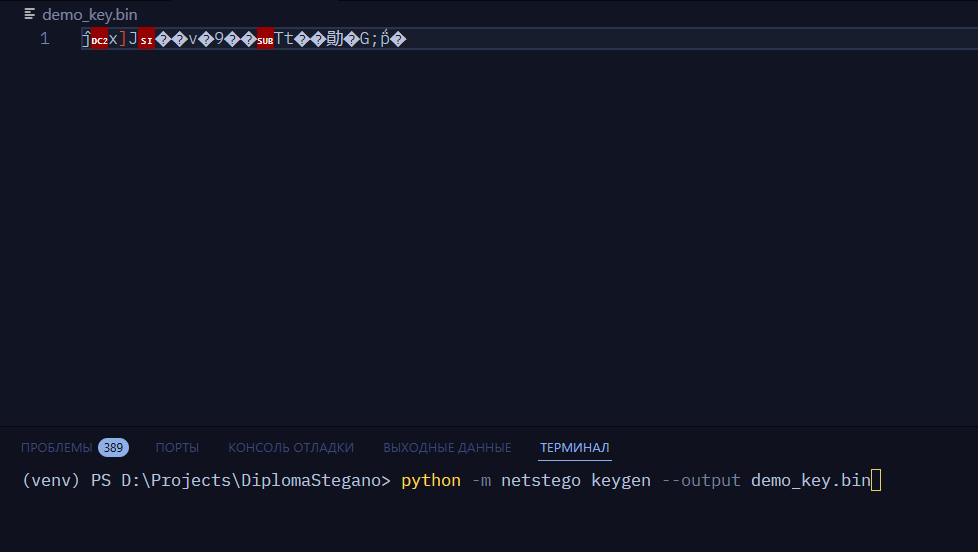
\includegraphics[width=0.85\textwidth]{demo_keygen.png}
\caption{Генерация 256-битного ключа шифрования}
\label{fig:demo_keygen}
\end{figure}

\subsubsection{Отправка сообщения через канал ICMP Payload}

Текстовое сообщение <<Secret message for NetStego demo>> (32~байта) передаётся через канал ICMP~Payload. Система выполняет шифрование AES-256-GCM (результат --- 60~байт шифротекста), фрагментацию на чанки с заголовком NST и кодирование в ICMP Echo Request пакет. Сформированные пакеты сохраняются в файл \texttt{demo\_icmp.pcap} (рисунок~\ref{fig:demo_send_icmp}).

\begin{figure}[htb]
\centering
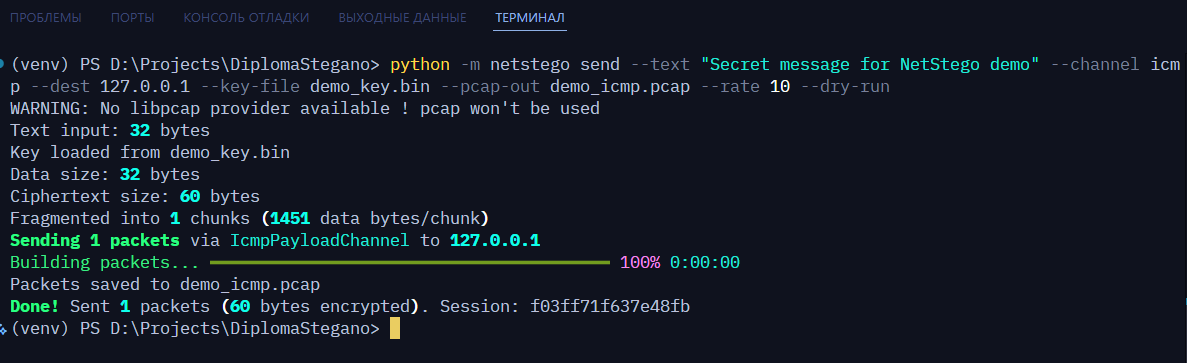
\includegraphics[width=0.85\textwidth]{demo_send_icmp.png}
\caption{Отправка текстового сообщения через канал ICMP Payload}
\label{fig:demo_send_icmp}
\end{figure}

\subsubsection{Приём и расшифровка сообщения (ICMP)}

Приём данных выполняется из сохранённого PCAP-файла с помощью команды \texttt{receive}. Система последовательно выполняет: чтение пакетов из PCAP, декодирование каналом ICMP, извлечение и сборку чанков, верификацию CRC32 и SHA-256, расшифрование AES-256-GCM. На рисунке~\ref{fig:demo_receive_icmp} видно, что из 1~пакета декодировано 113~байт, извлечён 1~чанк, собрано 60~байт шифротекста, после расшифровки получено 32~байта исходного текста. Команда \texttt{type received.txt} подтверждает побайтовое совпадение с исходным сообщением: <<Secret message for NetStego demo>>.

\begin{figure}[htb]
\centering
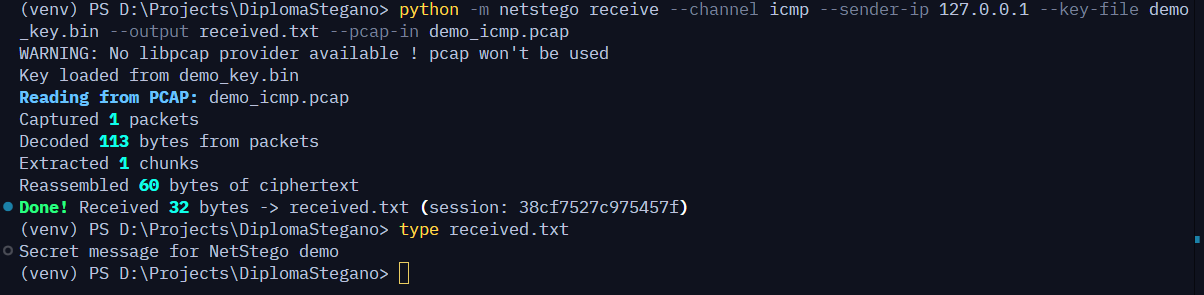
\includegraphics[width=0.85\textwidth]{demo_receive_icmp.png}
\caption{Приём и расшифровка сообщения из канала ICMP --- подтверждение целостности}
\label{fig:demo_receive_icmp}
\end{figure}

\subsubsection{Отправка файла через канал DNS QNAME}

Для демонстрации работы канала DNS QNAME в качестве входных данных используется текстовый файл. Система кодирует зашифрованные данные в base32-поддомены DNS-запросов. Ввиду меньшей ёмкости канала (30~байт на пакет) данные разбиваются на 3~чанка и формируют соответствующее количество DNS-пакетов (рисунок~\ref{fig:demo_send_dns}).

\begin{figure}[htb]
\centering
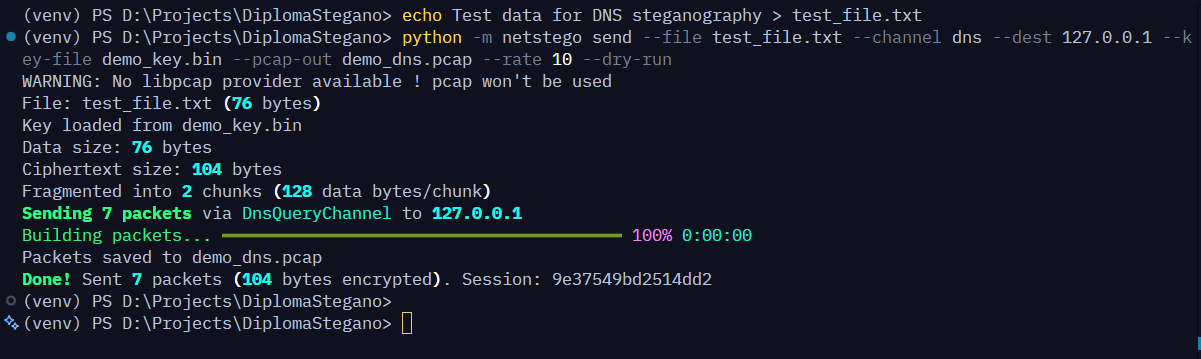
\includegraphics[width=0.85\textwidth]{demo_send_dns.png}
\caption{Отправка файла через канал DNS QNAME}
\label{fig:demo_send_dns}
\end{figure}

\subsubsection{Обнаружение скрытого канала в ICMP-трафике}

Модуль обнаружения анализирует файл \texttt{demo\_icmp.pcap} и выносит вердикт <<SUSPICIOUS>> с уровнем уверенности 70\,\%. Статистический анализ выявляет аномальный размер ICMP payload (115~байт --- нехарактерно для стандартных ICMP Echo Request). Сигнатурный анализ обнаруживает магическую последовательность \texttt{NST\textbackslash x00} протокола фрагментации в пакете~\#0 на смещении~6 (рисунок~\ref{fig:demo_detect_icmp}).

\begin{figure}[htb]
\centering
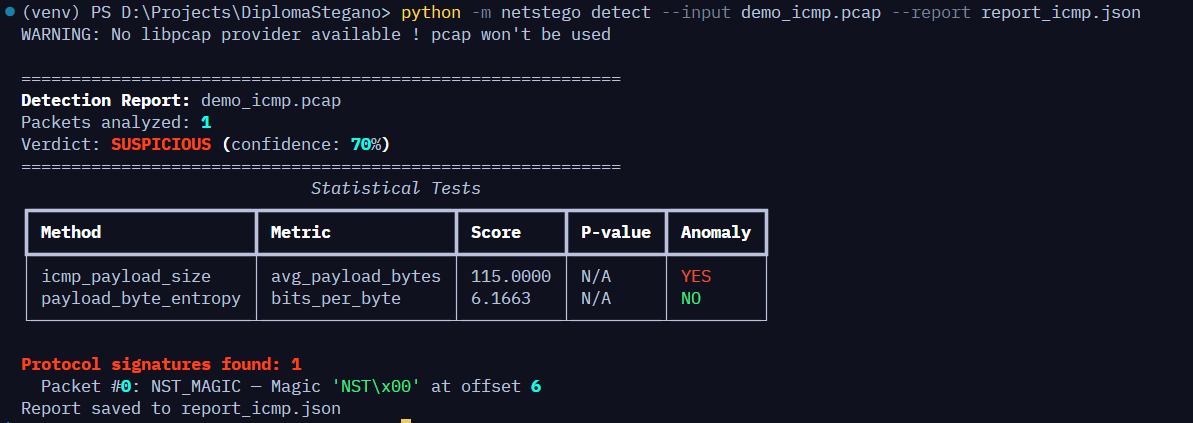
\includegraphics[width=0.85\textwidth]{demo_detect_icmp.png}
\caption{Результат обнаружения скрытого канала в ICMP-трафике}
\label{fig:demo_detect_icmp}
\end{figure}

\subsubsection{Обнаружение скрытого канала в DNS-трафике}

Анализ файла \texttt{demo\_dns.pcap} также выносит вердикт <<SUSPICIOUS>> с уровнем уверенности 70\,\%. Сигнатурный метод обнаруживает характерные для стеганографии base32-паттерны в DNS QNAME и терминационные маркеры. Статистический метод выявляет высокую энтропию поддоменов, нехарактерную для легитимного DNS-трафика (рисунок~\ref{fig:demo_detect_dns}).

\begin{figure}[htb]
\centering
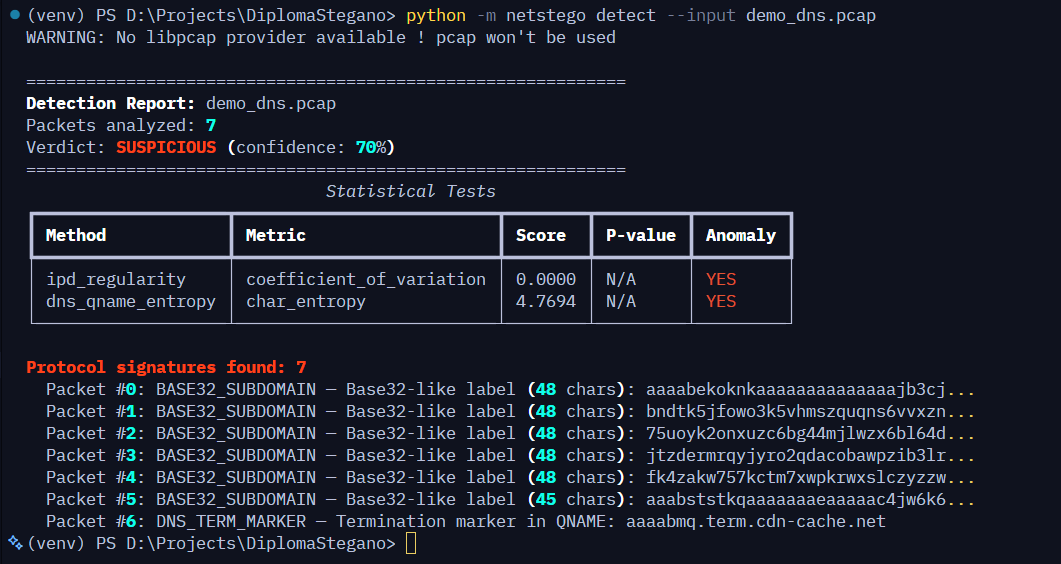
\includegraphics[width=0.85\textwidth]{demo_detect_dns.png}
\caption{Результат обнаружения скрытого канала в DNS-трафике}
\label{fig:demo_detect_dns}
\end{figure}

\subsubsection{Автоматизированное тестирование}

Для подтверждения корректности работы всех компонентов системы выполнен запуск полного набора автоматизированных тестов (рисунок~\ref{fig:demo_pytest}). Результат --- 269~тестов пройдено успешно (134~модульных, 68~интеграционных, 67~тестов целостности данных). Тесты покрывают все стеганографические каналы, криптографический модуль, протокол фрагментации и сборки, модуль обнаружения, систему бенчмарков и визуализации.

\begin{figure}[htb]
\centering
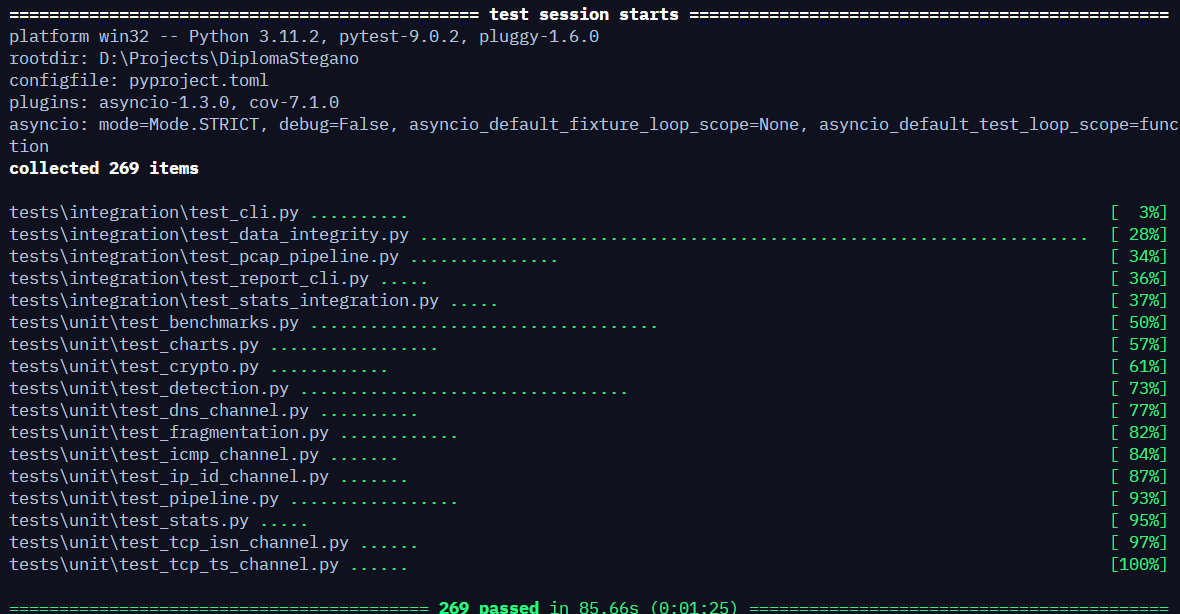
\includegraphics[width=0.85\textwidth]{demo_pytest.png}
\caption{Результат запуска автоматизированных тестов (269 passed)}
\label{fig:demo_pytest}
\end{figure}

Таким образом, демонстрация подтверждает полную работоспособность конвейера: исходное сообщение проходит этапы шифрования, фрагментации, стеганографического кодирования и обратного преобразования с побайтовым совпадением результата. Модуль обнаружения успешно выявляет скрытые каналы как в ICMP, так и в DNS-трафике.

\subsection{Выводы по реализации}

В результате работы реализована модульная и расширяемая система \texttt{NetStego}, включающая:
\begin{enumerate}[label=\arabic*)]
    \item пять стеганографических каналов с различными характеристиками ёмкости и скрытности, включая конфигурируемый DNS-суффикс для снижения обнаруживаемости;
    \item криптографическую защиту на основе AES-256-GCM с деривацией ключа Argon2id;
    \item протокол фрагментации с контролем целостности (CRC32, SHA-256) и поддержкой out-of-order сборки;
    \item многоуровневый модуль обнаружения, объединяющий статистический анализ (9~тестов), ML-обнаружение (Isolation Forest и Random Forest с 9~признаками) и сигнатурный поиск;
    \item модуль анализа содержимого payload для обнаружения вредоносных вложений (20~сигнатур в 7~категориях);
    \item систему сбора статистики с базой данных SQLite, интегрированную в конвейеры отправки и приёма;
    \item автоматическую генерацию 6~типов графиков и отчётов для демонстрации результатов;
    \item удобный CLI-интерфейс с 7~командами и поддержкой экспорта в JSON, CSV и HTML.
\end{enumerate}

Тестирование подтвердило корректность работы всех компонентов (269~тестов) и позволило оценить производительность каналов и эффективность методов обнаружения.

\newpage

%% Заключение
%%% conclusion.tex — Заключение
\section*{ЗАКЛЮЧЕНИЕ}
\addcontentsline{toc}{section}{ЗАКЛЮЧЕНИЕ}

Проведённое исследование подтвердило, что сетевая стеганография представляет реальную и труднообнаруживаемую угрозу для информационной безопасности корпоративных сетей. Анализ деятельности APT-группировок (Turla, Equation Group, APT29) показал, что скрытые каналы в протоколах TCP/IP активно эксплуатируются для управления вредоносным ПО и эксфильтрации данных, при этом существующие средства защиты (DPI, IDS/IPS, DLP) не обеспечивают их надёжного обнаружения.

Сравнительный анализ сетевой и контейнерной стеганографии выявил, что встраивание данных в поля заголовков пакетов, несмотря на существенно меньшую ёмкость по сравнению с мультимедийными контейнерами, обладает принципиальным преимуществом --- оно не создаёт новых информационных потоков и не требует передачи дополнительных файлов, что делает его практически невидимым для стандартных средств мониторинга. Данное свойство определяет целесообразность сетевой стеганографии для передачи малых объёмов критически важных данных в контролируемых сетевых средах.

Разработанная система \texttt{NetStego} реализует пять стеганографических каналов с ёмкостью от 2 до 1470~байт на пакет, покрывая диапазон от высокоскрытных (IP~ID, TCP~ISN, TCP~Timestamp) до высокоёмких (ICMP Payload) каналов. Эффективная пропускная способность варьируется от 20~байт/с до 115{,}9~Кбит/с при скорости 10~PPS, что подтверждает фундаментальный компромисс между скоростью передачи и скрытностью канала.

Применение криптографического алгоритма AES-256-GCM с деривацией ключа Argon2id и двухуровневого контроля целостности (CRC32 на уровне чанков, SHA-256 на уровне файла) обеспечивает конфиденциальность, аутентичность и целостность передаваемых данных. Протокол фрагментации NST с поддержкой сборки чанков не по порядку доставки обеспечивает устойчивость к переупорядочиванию пакетов в сети.

Модуль обнаружения скрытых каналов объединяет четыре метода детекции: статистический анализ (9~тестов, включая канал-специфичные проверки), алгоритм Isolation Forest (unsupervised, 9~признаков с учётом энтропии payload), алгоритм Random Forest (supervised, обучение на размеченных данных) и сигнатурный поиск. Результаты тестирования (269~тестов) продемонстрировали, что комбинация методов позволяет обнаруживать все реализованные каналы с F1-мерой от 0{,}80 до 0{,}90+ при уровне ложноположительных срабатываний не более 10\,\%.

Модуль анализа содержимого payload реализует обнаружение вредоносных вложений, скрытых в стеганографическом трафике. Сканирование извлечённых данных на наличие 20~сигнатур в 7~категориях (исполняемые файлы, скрипты, шеллкод, архивы, макро-документы, веб-атаки, обфускация) позволяет не только выявить факт использования скрытого канала, но и классифицировать тип скрытых данных для оценки уровня угрозы.

Реализованный механизм избыточности (дублирование чанков с дедупликацией по порядковому номеру) обеспечивает устойчивость к потере пакетов для высокоёмких каналов: при трёхкратной избыточности данные восстанавливаются при потере до 20\,\% пакетов. Система сбора статистики, интегрированная в конвейеры отправки и приёма, обеспечивает протоколирование каждой сессии в базе данных SQLite с поддержкой экспорта в JSON, CSV и HTML. Модуль визуализации автоматически генерирует 6~типов графиков для демонстрации результатов производительности и точности обнаружения.

Вместе с тем выявлены ограничения системы: отсутствие механизма ARQ для повторной передачи потерянных фрагментов, обнаруживаемость сигнатуры NST в полезной нагрузке высокоёмких каналов, а также уязвимость к активным нарушителям, способным модифицировать подозрительные пакеты. Устранение данных ограничений --- применение помехоустойчивого кодирования (Reed--Solomon), обфускация сигнатур и адаптивная маскировка временных характеристик --- определяет направления дальнейших исследований.

Практическая значимость работы состоит в создании инструмента, пригодного для исследования уязвимостей сетевых протоколов, обучения специалистов по кибербезопасности и тестирования корпоративных систем защиты. Реализованный модуль обнаружения, объединяющий статистический, ML и сигнатурный анализ с модулем обнаружения вредоносных вложений, может быть интегрирован с системами SIEM для автоматического выявления стеганографической активности и классификации скрытых угроз в реальном времени.

\textbf{Перспективы дальнейшего развития:}
\begin{enumerate}[label=\arabic*)]
    \item расширение набора каналов за счёт IPv6 Extension Headers, протоколов HTTP/2 и QUIC;
    \item реализация ARQ-протокола с использованием NACK-флага для повторной передачи;
    \item обфускация сигнатуры NST с помощью XOR-маски, производной от ключа;
    \item замена простого дублирования на коды коррекции ошибок (Reed--Solomon);
    \item использование глубокого обучения (CNN/LSTM) для анализа последовательностей пакетов;
    \item внедрение модуля обнаружения в режиме реального времени на основе высокопроизводительных фреймворков PF\_RING или DPDK;
    \item интеграция с системами SIEM для автоматического оповещения при обнаружении стеганографической активности.
\end{enumerate}

\newpage

%% Список использованных источников
%%% references.tex — Список использованных источников
\section*{СПИСОК ИСПОЛЬЗОВАННЫХ ИСТОЧНИКОВ}
\addcontentsline{toc}{section}{СПИСОК ИСПОЛЬЗОВАННЫХ ИСТОЧНИКОВ}

\begin{enumerate}
  \item Олифер~В.\,Г., Олифер~Н.\,А. Компьютерные сети. Принципы, технологии, протоколы~/ В.\,Г.~Олифер, Н.\,А.~Олифер.~--- 5-е изд.~--- СПб.\,: Питер, 2016.~--- 992~с.

  \item Таненбаум~Э., Уэзеролл~Д. Компьютерные сети~/ Э.~Таненбаум, Д.~Уэзеролл.~--- 6-е изд.~--- СПб.\,: Питер, 2023.~--- 960~с.

  \item Postel~J. Internet Protocol~/ J.~Postel~// RFC~791.~--- IETF, 1981.~--- 45~p.

  \item Postel~J. Transmission Control Protocol~/ J.~Postel~// RFC~793.~--- IETF, 1981.~--- 85~p.

  \item Postel~J. Internet Control Message Protocol~/ J.~Postel~// RFC~792.~--- IETF, 1981.~--- 21~p.

  \item Mockapetris~P. Domain Names~--- Implementation and Specification~/ P.~Mockapetris~// RFC~1035.~--- IETF, 1987.~--- 55~p.

  \item Borman~D., Braden~R., Jacobson~V., Scheffenegger~R. TCP Extensions for High Performance~/ D.~Borman, R.~Braden, V.~Jacobson, R.~Scheffenegger~// RFC~7323.~--- IETF, 2014.~--- 49~p.

  \item Dworkin~M. Recommendation for Block Cipher Modes of Operation: Galois/Counter Mode (GCM) and GMAC~/ M.~Dworkin~// NIST Special Publication 800-38D.~--- 2007.~--- 39~p.

  \item Biryukov~A., Dinu~D., Khovratovich~D. Argon2: Memory-Hard Function for Password Hashing and Proof-of-Work Applications~/ A.~Biryukov, D.~Dinu, D.~Khovratovich~// RFC~9106.~--- IETF, 2021.~--- 30~p.

  \item Touch~J. Updated Specification of the IPv4 ID Field~/ J.~Touch~// RFC~6528.~--- IETF, 2012.~--- 16~p.

  \item Zander~S., Armitage~G., Branch~P. A Survey of Covert Channels and Countermeasures in Computer Network Protocols~/ S.~Zander, G.~Armitage, P.~Branch~// IEEE Communications Surveys \& Tutorials.~--- 2007.~--- Vol.~9, No.~3.~--- P.~44--57.

  \item Mazurczyk~W., Caviglione~L. Information Hiding as a Challenge for Malware Detection~/ W.~Mazurczyk, L.~Caviglione~// IEEE Security \& Privacy.~--- 2015.~--- Vol.~13, No.~2.~--- P.~89--93.

  \item Positive Technologies. Актуальные киберугрозы: итоги 2024 года~/ Positive Technologies.~--- [Электронный ресурс].~--- URL: \url{https://www.ptsecurity.com/ru-ru/research/analytics/} (дата обращения: 15.03.2026).

  \item Bencs\'{a}th~B., P\'{e}k~G., Butty\'{a}n~L., F\'{e}legyh\'{a}zi~M. Duqu: Analysis, Detection, and Lessons Learned~/ B.~Bencs\'{a}th, G.~P\'{e}k, L.~Butty\'{a}n, M.~F\'{e}legyh\'{a}zi~// ACM European Workshop on System Security (EuroSec).~--- 2012.~--- P.~1--6.

  \item Kaspersky Lab. ProjectSauron: Top Level Cyber-Espionage Platform Covertly Extracts Encrypted Government Communications~/ Kaspersky Lab.~--- Technical Report, 2016.~--- 23~p.

  \item Kaspersky Lab. Equation Group: Questions and Answers~/ GReAT, Kaspersky Lab.~--- Technical Report, 2015.~--- 44~p.

  \item Lampson~B.\,W. A Note on the Confinement Problem~/ B.\,W.~Lampson~// Communications of the ACM.~--- 1973.~--- Vol.~16, No.~10.~--- P.~613--615.

  \item Bellovin~S. Defending Against Sequence Number Attacks~/ S.~Bellovin~// RFC~1948.~--- IETF, 1996.~--- 6~p.

  \item Liu~B., Zhai~L., Wang~R. Network Covert Channel Detection Based on Isolation Forest~/ B.~Liu, L.~Zhai, R.~Wang~// Proc. International Conference on Network Security (ICNS).~--- 2019.~--- P.~112--118.

  \item Fisk~G., Fisk~M., Papadopoulos~C., Neil~J. Eliminating Steganography in Internet Traffic with Active Wardens~/ G.~Fisk, M.~Fisk, C.~Papadopoulos, J.~Neil~// Proc. International Workshop on Information Hiding (IH).~--- Springer LNCS, 2002.~--- P.~18--35.

  \item Scapy Project. Scapy Documentation~/ Scapy Project.~--- [Электронный ресурс].~--- URL: \url{https://scapy.readthedocs.io/} (дата обращения: 24.03.2026).

  \item Cryptography.io. Cryptography Library Documentation~/ PyCA.~--- [Электронный ресурс].~--- URL: \url{https://cryptography.io/} (дата обращения: 24.03.2026).

  \item Pedregosa~F., Varoquaux~G., Gramfort~A. et~al. Scikit-learn: Machine Learning in Python~/ F.~Pedregosa, G.~Varoquaux, A.~Gramfort [et~al.]~// Journal of Machine Learning Research.~--- 2011.~--- Vol.~12.~--- P.~2825--2830.
\end{enumerate}

\newpage

%% Приложения
%%% appendix.tex — Приложения (полный исходный код системы NetStego)
\newpage
\section*{ПРИЛОЖЕНИЕ А. Модуль обнаружения стеганографических каналов}
\addcontentsline{toc}{section}{ПРИЛОЖЕНИЕ А. Модуль обнаружения стеганографических каналов}

Модуль \texttt{detection/analyzer.py} является центральным компонентом
подсистемы обнаружения скрытых каналов. Оркестрирует работу статистических
тестов, машинного обучения и сигнатурного анализа, вычисляет взвешенную
оценку уверенности и формирует итоговый отчёт.

\begin{lstlisting}[style=appendixcode]
"""Detection orchestrator: combines statistical, ML, and signature methods.

Analyzes PCAP files or live packet captures for signs of
steganographic covert channels.
"""

import json
from dataclasses import dataclass, field
from pathlib import Path

from rich.console import Console
from rich.table import Table
from scapy.layers.dns import DNSQR
from scapy.layers.inet import ICMP, IP, TCP
from scapy.packet import Raw
from scapy.utils import rdpcap

from netstego.detection.ml_detector import (
    MLResult, detect_isolation_forest, extract_features,
)
from netstego.detection.signatures import (
    SignatureMatch, detect_signatures,
)
from netstego.detection.statistical import (
    StatResult, chi_squared_uniformity, ipd_regularity,
    ks_test_ipd, shannon_entropy,
)

console = Console()


@dataclass
class AnalysisReport:
    """Complete analysis report."""

    source: str
    total_packets: int
    statistical_results: list[StatResult] = field(
        default_factory=list
    )
    ml_result: MLResult | None = None
    signature_matches: list[SignatureMatch] = field(
        default_factory=list
    )
    is_suspicious: bool = False
    confidence: float = 0.0

    def to_dict(self) -> dict:
        """Serialize report to dictionary."""
        proto_sigs = [
            m for m in self.signature_matches
            if m.field != "payload_content"
        ]
        content_sigs = [
            m for m in self.signature_matches
            if m.field == "payload_content"
        ]
        return {
            "source": self.source,
            "total_packets": self.total_packets,
            "is_suspicious": self.is_suspicious,
            "confidence": self.confidence,
            "statistical": [
                {
                    "method": r.method,
                    "metric": r.metric,
                    "score": r.score,
                    "p_value": r.p_value,
                    "is_anomaly": r.is_anomaly,
                    "details": r.details,
                }
                for r in self.statistical_results
            ],
            "ml": {
                "method": self.ml_result.method,
                "anomaly_ratio": self.ml_result.anomaly_ratio,
                "is_anomaly": self.ml_result.is_anomaly,
                "details": self.ml_result.details,
            }
            if self.ml_result
            else None,
            "signatures": [
                {
                    "packet_index": m.packet_index,
                    "pattern": m.pattern,
                    "confidence": m.confidence,
                    "details": m.details,
                }
                for m in proto_sigs
            ],
            "content_analysis": [
                {
                    "packet_index": m.packet_index,
                    "pattern": m.pattern,
                    "confidence": m.confidence,
                    "details": m.details,
                }
                for m in content_sigs
            ],
        }


def _extract_packet_data(packets: list) -> dict:
    """Extract field values, timestamps, and payloads from packets.

    Returns dict with keys: ip_ids, tcp_seqs, timestamps,
    payloads, ipds, sizes, tcp_tsvals, dns_qnames,
    icmp_payload_sizes.
    """
    ip_ids = []
    tcp_seqs = []
    tcp_tsvals = []
    dns_qnames = []
    icmp_payload_sizes = []
    timestamps = []
    payloads = []
    sizes = []

    for pkt in packets:
        if pkt.haslayer(IP):
            ip_ids.append(pkt[IP].id)
        if pkt.haslayer(TCP):
            tcp_seqs.append(pkt[TCP].seq)
            for opt_name, opt_val in pkt[TCP].options:
                if opt_name == "Timestamp":
                    tcp_tsvals.append(opt_val[0])
                    break
        if pkt.haslayer(DNSQR):
            qname = pkt[DNSQR].qname
            if isinstance(qname, bytes):
                qname = qname.decode(
                    "ascii", errors="ignore"
                )
            dns_qnames.append(qname.rstrip("."))
        if pkt.haslayer(ICMP) and pkt.haslayer(Raw):
            icmp_payload_sizes.append(
                len(bytes(pkt[Raw].load))
            )
        ts = (
            float(pkt.time)
            if hasattr(pkt, "time")
            else 0.0
        )
        timestamps.append(ts)
        if pkt.haslayer(Raw):
            payloads.append(bytes(pkt[Raw].load))
        else:
            payloads.append(b"")
        sizes.append(len(pkt))

    ipds = [
        timestamps[i] - timestamps[i - 1]
        for i in range(1, len(timestamps))
    ]
    return {
        "ip_ids": ip_ids,
        "tcp_seqs": tcp_seqs,
        "tcp_tsvals": tcp_tsvals,
        "dns_qnames": dns_qnames,
        "icmp_payload_sizes": icmp_payload_sizes,
        "timestamps": timestamps,
        "payloads": payloads,
        "ipds": ipds,
        "sizes": sizes,
    }


def _ip_id_sequentiality(ip_ids: list[int]) -> StatResult:
    """Check if IP ID values follow a sequential pattern.

    Normal Windows traffic: IP ID increments by 1-3.
    Stego: arbitrary values that break sequential patterns.
    """
    if len(ip_ids) < 3:
        return StatResult(
            method="ip_id_sequentiality",
            metric="sequential_ratio",
            score=0.0, p_value=None,
            threshold=0.0, is_anomaly=False,
            details="Insufficient data",
        )
    sequential_count = 0
    for i in range(1, len(ip_ids)):
        delta = (ip_ids[i] - ip_ids[i - 1]) % 65536
        if 1 <= delta <= 10:
            sequential_count += 1
    ratio = sequential_count / (len(ip_ids) - 1)
    threshold = 0.3
    return StatResult(
        method="ip_id_sequentiality",
        metric="sequential_ratio",
        score=ratio, p_value=None,
        threshold=threshold,
        is_anomaly=ratio < threshold,
        details=(
            f"sequential_pairs="
            f"{sequential_count}/{len(ip_ids)-1}, "
            f"ratio={ratio:.4f}"
        ),
    )


def _tsval_monotonicity(
    tsvals: list[int],
) -> StatResult:
    """Check if TCP TSval is monotonically increasing.

    Normal: monotonic with consistent step.
    Stego: arbitrary data breaking monotonicity.
    """
    violations = 0
    for i in range(1, len(tsvals)):
        if tsvals[i] <= tsvals[i - 1]:
            violations += 1
    ratio = (
        violations / (len(tsvals) - 1)
        if len(tsvals) > 1
        else 0.0
    )
    threshold = 0.2
    return StatResult(
        method="tsval_monotonicity",
        metric="violation_ratio",
        score=ratio, p_value=None,
        threshold=threshold,
        is_anomaly=ratio > threshold,
        details=(
            f"violations={violations}/"
            f"{len(tsvals)-1}, ratio={ratio:.4f}"
        ),
    )


def _dns_qname_entropy(
    qnames: list[str],
) -> StatResult:
    """Check entropy of DNS QNAME characters.

    Normal DNS: readable names, low entropy (~3.5-4.0).
    Base32 stego: random, high entropy (~4.5-5.0).
    """
    import math

    all_chars = "".join(qnames)
    if not all_chars:
        return StatResult(
            method="dns_qname_entropy",
            metric="char_entropy",
            score=0.0, p_value=None,
            threshold=0.0, is_anomaly=False,
            details="No data",
        )
    freq: dict[str, int] = {}
    for c in all_chars:
        freq[c] = freq.get(c, 0) + 1
    n = len(all_chars)
    entropy = -sum(
        (cnt / n) * math.log2(cnt / n)
        for cnt in freq.values()
    )
    avg_len = sum(len(q) for q in qnames) / len(qnames)
    threshold_entropy = 4.3
    threshold_len = 25
    is_anomaly = (
        entropy > threshold_entropy
        and avg_len > threshold_len
    )
    return StatResult(
        method="dns_qname_entropy",
        metric="char_entropy",
        score=entropy, p_value=None,
        threshold=threshold_entropy,
        is_anomaly=is_anomaly,
        details=(
            f"H={entropy:.4f}, "
            f"avg_qname_len={avg_len:.1f}, "
            f"unique_chars={len(freq)}"
        ),
    )


def _icmp_payload_anomaly(
    payload_sizes: list[int],
) -> StatResult:
    """Check if ICMP payload sizes are abnormal.

    Normal ping: 32 bytes (Win) or 56 bytes (Linux).
    Stego: often much larger (up to 1472 bytes).
    """
    avg_size = sum(payload_sizes) / len(payload_sizes)
    max_size = max(payload_sizes)
    threshold = 100
    is_anomaly = avg_size > threshold
    return StatResult(
        method="icmp_payload_size",
        metric="avg_payload_bytes",
        score=avg_size, p_value=None,
        threshold=float(threshold),
        is_anomaly=is_anomaly,
        details=(
            f"avg={avg_size:.0f}, max={max_size}, "
            f"count={len(payload_sizes)}"
        ),
    )


def _payload_byte_entropy(
    payloads: list[bytes],
) -> StatResult:
    """Check byte-level entropy of packet payloads.

    Encrypted stego data: entropy close to 8.0 bits/byte.
    Normal ICMP: repeating pattern, much lower entropy.
    """
    import math

    all_bytes = b"".join(payloads)
    if not all_bytes:
        return StatResult(
            method="payload_byte_entropy",
            metric="bits_per_byte",
            score=0.0, p_value=None,
            threshold=0.0, is_anomaly=False,
            details="No data",
        )
    freq = [0] * 256
    for b in all_bytes:
        freq[b] += 1
    n = len(all_bytes)
    entropy = -sum(
        (f / n) * math.log2(f / n) for f in freq if f > 0
    )
    threshold = 7.0
    return StatResult(
        method="payload_byte_entropy",
        metric="bits_per_byte",
        score=entropy, p_value=None,
        threshold=threshold,
        is_anomaly=entropy > threshold,
        details=(
            f"H={entropy:.4f} bits/byte, "
            f"total_bytes={n}"
        ),
    )


def _detect_dns_stego_signatures(
    qnames: list[str],
) -> list:
    """Detect stego patterns in DNS QNAME labels."""
    import re
    from netstego.detection.signatures import (
        SignatureMatch,
    )

    matches = []
    base32_pattern = re.compile(r"^[a-z2-7]{20,}$")
    for i, qname in enumerate(qnames):
        labels = qname.split(".")
        for label in labels[:-2]:
            if (
                base32_pattern.match(label)
                and len(label) > 20
            ):
                matches.append(SignatureMatch(
                    packet_index=i,
                    field="dns_qname",
                    pattern="BASE32_SUBDOMAIN",
                    confidence=0.85,
                    details=(
                        f"Base32-like label "
                        f"({len(label)} chars): "
                        f"{label[:30]}..."
                    ),
                ))
                break
        if any(l == "term" for l in labels):
            matches.append(SignatureMatch(
                packet_index=i,
                field="dns_qname",
                pattern="DNS_TERM_MARKER",
                confidence=0.9,
                details=(
                    f"Termination marker "
                    f"in QNAME: {qname}"
                ),
            ))
    return matches


def analyze_packets(
    packets: list,
    source: str = "unknown",
    methods: list[str] | None = None,
    alpha: float = 0.05,
    ml_contamination: float = 0.05,
) -> AnalysisReport:
    """Run detection analysis on a list of packets.

    Args:
        packets: List of Scapy packets.
        source: Source description (file path or iface).
        methods: Methods to run: 'statistical',
                 'ml', 'signatures'. Default: all.
        alpha: Significance level for stat tests.
        ml_contamination: IsolationForest parameter.

    Returns:
        AnalysisReport with all results.
    """
    if methods is None:
        methods = ["statistical", "ml", "signatures"]

    report = AnalysisReport(
        source=source, total_packets=len(packets)
    )
    data = _extract_packet_data(packets)

    # Statistical tests
    if "statistical" in methods:
        if (
            data["ip_ids"]
            and len(data["ip_ids"]) >= 10
        ):
            report.statistical_results.append(
                _ip_id_sequentiality(data["ip_ids"])
            )
        if (
            data["tcp_seqs"]
            and len(data["tcp_seqs"]) >= 10
        ):
            report.statistical_results.append(
                chi_squared_uniformity(
                    data["tcp_seqs"], alpha
                )
            )
        if data["ipds"]:
            report.statistical_results.append(
                ipd_regularity(data["ipds"])
            )
        if (
            data["tcp_tsvals"]
            and len(data["tcp_tsvals"]) >= 3
        ):
            report.statistical_results.append(
                _tsval_monotonicity(data["tcp_tsvals"])
            )
        if (
            data["dns_qnames"]
            and len(data["dns_qnames"]) >= 3
        ):
            report.statistical_results.append(
                _dns_qname_entropy(data["dns_qnames"])
            )
        if (
            data["icmp_payload_sizes"]
            and len(data["icmp_payload_sizes"]) >= 1
        ):
            report.statistical_results.append(
                _icmp_payload_anomaly(
                    data["icmp_payload_sizes"]
                )
            )
        icmp_payloads = [
            p for p in data["payloads"] if len(p) > 40
        ]
        if icmp_payloads:
            report.statistical_results.append(
                _payload_byte_entropy(icmp_payloads)
            )

    # ML detection
    if "ml" in methods:
        field_values = (
            data["ip_ids"]
            or data["tcp_seqs"]
            or [0] * len(packets)
        )
        features = extract_features(
            field_values, data["timestamps"],
            data["sizes"], data["payloads"],
        )
        if len(features) >= 10:
            report.ml_result = detect_isolation_forest(
                features, ml_contamination
            )

    # Signature detection
    if "signatures" in methods:
        report.signature_matches = detect_signatures(
            data["payloads"]
        )
        if data["dns_qnames"]:
            report.signature_matches.extend(
                _detect_dns_stego_signatures(
                    data["dns_qnames"]
                )
            )

    # Compute overall suspicion
    import math as _math

    valid_stats = [
        r
        for r in report.statistical_results
        if "Insufficient" not in r.details
        and "No data" not in r.details
        and (
            r.p_value is None
            or not _math.isnan(r.p_value)
        )
        and "bins=1" not in r.details
    ]
    anomaly_count = sum(
        1 for r in valid_stats if r.is_anomaly
    )
    total_tests = len(valid_stats)
    stat_ratio = (
        anomaly_count / total_tests
        if total_tests > 0
        else 0.0
    )

    strong_indicators = {
        r.method for r in valid_stats if r.is_anomaly
    } & {
        "tsval_monotonicity",
        "dns_qname_entropy",
        "icmp_payload_size",
        "payload_byte_entropy",
        "ip_id_sequentiality",
    }

    ml_suspicious = (
        report.ml_result.is_anomaly
        if report.ml_result
        else False
    )
    sig_count = len(report.signature_matches)

    confidence = 0.0
    if stat_ratio >= 0.5 or len(strong_indicators) >= 1:
        confidence += 0.4
    if ml_suspicious:
        confidence += 0.3
    if sig_count > 0:
        confidence += 0.3

    report.is_suspicious = confidence >= 0.4
    report.confidence = confidence

    return report


def analyze_pcap(
    pcap_path: Path,
    methods: list[str] | None = None,
    alpha: float = 0.05,
    ml_contamination: float = 0.05,
) -> AnalysisReport:
    """Analyze a PCAP file for covert channels."""
    packets = rdpcap(str(pcap_path))
    return analyze_packets(
        list(packets),
        source=str(pcap_path),
        methods=methods,
        alpha=alpha,
        ml_contamination=ml_contamination,
    )


def print_report(report: AnalysisReport) -> None:
    """Print analysis report to console using rich."""
    verdict = (
        "[bold red]SUSPICIOUS[/bold red]"
        if report.is_suspicious
        else "[bold green]CLEAN[/bold green]"
    )
    console.print(f"\n{'='*60}")
    console.print(
        f"[bold]Detection Report:[/bold] "
        f"{report.source}"
    )
    console.print(
        f"Packets analyzed: {report.total_packets}"
    )
    console.print(
        f"Verdict: {verdict} "
        f"(confidence: {report.confidence:.0%})"
    )
    console.print(f"{'='*60}")

    if report.statistical_results:
        table = Table(title="Statistical Tests")
        table.add_column("Method")
        table.add_column("Metric")
        table.add_column("Score")
        table.add_column("P-value")
        table.add_column("Anomaly")
        for r in report.statistical_results:
            style = "red" if r.is_anomaly else "green"
            table.add_row(
                r.method, r.metric,
                f"{r.score:.4f}",
                (
                    f"{r.p_value:.6f}"
                    if r.p_value is not None
                    else "N/A"
                ),
                f"[{style}]"
                f"{'YES' if r.is_anomaly else 'NO'}"
                f"[/{style}]",
            )
        console.print(table)

    if report.ml_result:
        ml = report.ml_result
        style = "red" if ml.is_anomaly else "green"
        console.print(
            f"\n[bold]ML Detection "
            f"({ml.method}):[/bold]"
        )
        console.print(
            f"  Anomaly ratio: "
            f"[{style}]{ml.anomaly_ratio:.2%}"
            f"[/{style}]"
        )
        console.print(f"  Details: {ml.details}")

    proto_sigs = [
        m for m in report.signature_matches
        if m.field != "payload_content"
    ]
    content_sigs = [
        m for m in report.signature_matches
        if m.field == "payload_content"
    ]
    if proto_sigs:
        console.print(
            f"\n[bold red]Protocol signatures "
            f"found: {len(proto_sigs)}[/bold red]"
        )
        for m in proto_sigs[:10]:
            console.print(
                f"  Packet #{m.packet_index}: "
                f"{m.pattern} -- {m.details}"
            )
    if content_sigs:
        console.print(
            f"\n[bold red]Malicious content "
            f"indicators: {len(content_sigs)}"
            f"[/bold red]"
        )
        for m in content_sigs[:10]:
            console.print(
                f"  Packet #{m.packet_index}: "
                f"[bold]{m.pattern}[/bold] "
                f"(confidence: {m.confidence:.0%})"
                f" -- {m.details}"
            )
\end{lstlisting}

\newpage
\section*{ПРИЛОЖЕНИЕ Б. Модули статистического анализа, машинного обучения и сигнатурного обнаружения}
\addcontentsline{toc}{section}{ПРИЛОЖЕНИЕ Б. Модули статистического анализа, машинного обучения и сигнатурного обнаружения}

\subsection*{Б.1 Статистические методы обнаружения (\texttt{detection/statistical.py})}

Модуль реализует четыре статистических теста: критерий хи-квадрат
для проверки равномерности распределения значений полей,
критерий Колмогорова--Смирнова для анализа межпакетных задержек,
вычисление энтропии Шеннона и анализ регулярности задержек.

\begin{lstlisting}[style=appendixcode]
"""Statistical detection methods for covert channel
analysis.

Implements:
    - Chi-squared test for field value distributions
    - Kolmogorov-Smirnov test for inter-packet delay
    - Shannon entropy calculation
    - Inter-packet delay analysis
"""

import math
from dataclasses import dataclass

import numpy as np
from scipy import stats as sp_stats


@dataclass
class StatResult:
    """Result of a statistical test."""

    method: str
    metric: str
    score: float
    p_value: float | None
    threshold: float
    is_anomaly: bool
    details: str = ""


def chi_squared_uniformity(
    values: list[int], alpha: float = 0.05,
) -> StatResult:
    """Chi-squared test for uniformity of field values.

    Tests whether the distribution of values deviates
    significantly from a uniform distribution, which
    may indicate steganographic encoding.
    """
    if len(values) < 10:
        return StatResult(
            method="chi_squared",
            metric="uniformity",
            score=0.0, p_value=1.0,
            threshold=alpha, is_anomaly=False,
            details="Insufficient data (< 10 samples)",
        )

    arr = np.array(values)
    n_bins = min(256, len(set(values)))
    observed, bin_edges = np.histogram(
        arr, bins=n_bins
    )
    expected = np.full_like(
        observed,
        fill_value=len(values) / n_bins,
        dtype=float,
    )
    chi2, p_value = sp_stats.chisquare(
        observed, f_exp=expected
    )
    return StatResult(
        method="chi_squared",
        metric="uniformity",
        score=float(chi2),
        p_value=float(p_value),
        threshold=alpha,
        is_anomaly=p_value < alpha,
        details=(
            f"chi2={chi2:.4f}, p={p_value:.6f}, "
            f"bins={n_bins}"
        ),
    )


def ks_test_ipd(
    delays: list[float], alpha: float = 0.05,
) -> StatResult:
    """Kolmogorov-Smirnov test for IPD distribution.

    Tests whether IPD follows an exponential
    distribution (typical for normal traffic).
    Steganographic traffic has more regular timing.
    """
    if len(delays) < 10:
        return StatResult(
            method="ks_test",
            metric="ipd_distribution",
            score=0.0, p_value=1.0,
            threshold=alpha, is_anomaly=False,
            details="Insufficient data (< 10 samples)",
        )

    arr = np.array(delays)
    arr = arr[arr > 0]
    if len(arr) < 5:
        return StatResult(
            method="ks_test",
            metric="ipd_distribution",
            score=0.0, p_value=1.0,
            threshold=alpha, is_anomaly=False,
            details="Insufficient positive delays",
        )

    mean_delay = float(np.mean(arr))
    stat, p_value = sp_stats.kstest(
        arr, "expon", args=(0, mean_delay)
    )
    return StatResult(
        method="ks_test",
        metric="ipd_distribution",
        score=float(stat),
        p_value=float(p_value),
        threshold=alpha,
        is_anomaly=p_value < alpha,
        details=(
            f"D={stat:.4f}, p={p_value:.6f}, "
            f"mean_ipd={mean_delay:.4f}s"
        ),
    )


def shannon_entropy(
    values: list[int],
) -> StatResult:
    """Calculate Shannon entropy of field values.

    High entropy close to theoretical maximum may
    indicate steganographic encoding.
    """
    if not values:
        return StatResult(
            method="entropy",
            metric="shannon",
            score=0.0, p_value=None,
            threshold=0.0, is_anomaly=False,
            details="No data",
        )

    n = len(values)
    freq: dict[int, int] = {}
    for v in values:
        freq[v] = freq.get(v, 0) + 1

    entropy = 0.0
    for count in freq.values():
        p = count / n
        if p > 0:
            entropy -= p * math.log2(p)

    max_entropy = math.log2(n) if n > 1 else 1.0
    normalized = (
        entropy / max_entropy
        if max_entropy > 0
        else 0.0
    )
    threshold = 0.95
    return StatResult(
        method="entropy",
        metric="shannon",
        score=normalized,
        p_value=None,
        threshold=threshold,
        is_anomaly=normalized > threshold,
        details=(
            f"H={entropy:.4f} bits, "
            f"normalized={normalized:.4f}, "
            f"unique={len(freq)}"
        ),
    )


def ipd_regularity(
    delays: list[float],
) -> StatResult:
    """Measure regularity of inter-packet delays.

    Low coefficient of variation (CV) suggests
    artificially timed traffic.
    """
    if len(delays) < 5:
        return StatResult(
            method="ipd_regularity",
            metric="coefficient_of_variation",
            score=0.0, p_value=None,
            threshold=0.0, is_anomaly=False,
            details="Insufficient data",
        )

    arr = np.array(delays)
    mean = float(np.mean(arr))
    std = float(np.std(arr))
    cv = std / mean if mean > 0 else 0.0

    threshold = 0.1
    return StatResult(
        method="ipd_regularity",
        metric="coefficient_of_variation",
        score=cv, p_value=None,
        threshold=threshold,
        is_anomaly=cv < threshold,
        details=(
            f"CV={cv:.4f}, mean={mean:.4f}s, "
            f"std={std:.4f}s"
        ),
    )
\end{lstlisting}

\newpage
\subsection*{Б.2 Обнаружение на основе машинного обучения}
\noindent Модуль \texttt{detection/ml\_detector.py}

Модуль реализует два метода обнаружения на основе машинного обучения:
Isolation Forest (обучение без учителя) и Random Forest (обучение
с учителем). Извлекает 9-мерный вектор признаков из пакетных данных.

\begin{lstlisting}[style=appendixcode]
"""Machine learning based covert channel detection.

Uses IsolationForest for anomaly detection on packet
features. Can optionally train a RandomForest classifier
if labeled data is available.
"""

from dataclasses import dataclass

import numpy as np
from sklearn.ensemble import (
    IsolationForest, RandomForestClassifier,
)
from sklearn.preprocessing import StandardScaler


@dataclass
class MLResult:
    """Result of ML-based detection."""

    method: str
    anomaly_ratio: float
    predictions: list[int]
    confidence: float
    is_anomaly: bool
    details: str = ""


def _byte_entropy(data: bytes) -> float:
    """Shannon entropy of byte values (0-8 bits/byte)."""
    if not data:
        return 0.0
    freq = [0] * 256
    for b in data:
        freq[b] += 1
    n = len(data)
    import math
    return -sum(
        (f / n) * math.log2(f / n)
        for f in freq
        if f > 0
    )


def extract_features(
    field_values: list[int],
    timestamps: list[float],
    packet_sizes: list[int] | None = None,
    payloads: list[bytes] | None = None,
) -> np.ndarray:
    """Extract feature vectors from packet data.

    Features per packet (sliding window of 5):
        - Field value
        - Delta from previous value
        - Inter-packet delay
        - Packet size
        - Rolling mean of field values
        - Rolling std of field values
        - Rolling mean of IPD
        - Payload byte entropy (0-8 bits/byte)
        - Payload length

    Returns:
        2D numpy array of shape (n_samples, 9).
    """
    n = len(field_values)
    if n < 2:
        return np.empty((0, 9))

    values = np.array(field_values, dtype=float)
    times = np.array(timestamps, dtype=float)
    sizes = (
        np.array(packet_sizes, dtype=float)
        if packet_sizes
        else np.zeros(n)
    )

    if payloads and len(payloads) == n:
        payload_entropies = np.array(
            [_byte_entropy(p) for p in payloads]
        )
        payload_lengths = np.array(
            [len(p) for p in payloads], dtype=float
        )
    else:
        payload_entropies = np.zeros(n)
        payload_lengths = np.zeros(n)

    value_deltas = np.diff(values, prepend=values[0])
    ipd = np.diff(times, prepend=times[0])

    window = min(5, n)
    features = []
    for i in range(n):
        start = max(0, i - window + 1)
        win_vals = values[start : i + 1]
        win_ipd = ipd[start : i + 1]
        features.append([
            values[i],
            value_deltas[i],
            ipd[i],
            sizes[i],
            float(np.mean(win_vals)),
            float(np.std(win_vals)),
            float(np.mean(win_ipd)),
            payload_entropies[i],
            payload_lengths[i],
        ])

    return np.array(features)


def detect_isolation_forest(
    features: np.ndarray,
    contamination: float = 0.05,
) -> MLResult:
    """Run IsolationForest anomaly detection."""
    if len(features) < 10:
        return MLResult(
            method="isolation_forest",
            anomaly_ratio=0.0, predictions=[],
            confidence=0.0, is_anomaly=False,
            details="Insufficient data (< 10 samples)",
        )

    scaler = StandardScaler()
    scaled = scaler.fit_transform(features)

    clf = IsolationForest(
        contamination=contamination,
        random_state=42,
        n_estimators=100,
    )
    predictions = clf.fit_predict(scaled)
    scores = clf.decision_function(scaled)

    anomaly_count = int(np.sum(predictions == -1))
    anomaly_ratio = anomaly_count / len(predictions)
    mean_score = float(np.mean(scores))

    return MLResult(
        method="isolation_forest",
        anomaly_ratio=anomaly_ratio,
        predictions=predictions.tolist(),
        confidence=abs(mean_score),
        is_anomaly=anomaly_ratio > contamination * 2,
        details=(
            f"anomalies={anomaly_count}/"
            f"{len(predictions)}, "
            f"ratio={anomaly_ratio:.4f}, "
            f"mean_score={mean_score:.4f}"
        ),
    )


def train_classifier(
    features: np.ndarray,
    labels: np.ndarray,
) -> tuple[RandomForestClassifier, StandardScaler]:
    """Train a RandomForest classifier on labeled data.

    Returns:
        Tuple of (trained classifier, fitted scaler).
    """
    scaler = StandardScaler()
    scaled = scaler.fit_transform(features)

    clf = RandomForestClassifier(
        n_estimators=100,
        random_state=42,
        max_depth=10,
    )
    clf.fit(scaled, labels)
    return clf, scaler


def detect_random_forest(
    train_features: np.ndarray,
    train_labels: np.ndarray,
    test_features: np.ndarray,
    test_labels: np.ndarray | None = None,
) -> MLResult:
    """Run supervised RandomForest detection.

    Trains on labeled normal/stego data and predicts
    test samples.
    """
    if (
        len(train_features) < 10
        or len(test_features) < 2
    ):
        return MLResult(
            method="random_forest",
            anomaly_ratio=0.0, predictions=[],
            confidence=0.0, is_anomaly=False,
            details=(
                "Insufficient data for supervised "
                "classification"
            ),
        )

    clf, scaler = train_classifier(
        train_features, train_labels
    )
    scaled_test = scaler.transform(test_features)
    predictions = clf.predict(scaled_test)
    probabilities = clf.predict_proba(scaled_test)

    stego_count = int(np.sum(predictions == 1))
    stego_ratio = (
        stego_count / len(predictions)
        if len(predictions) > 0
        else 0.0
    )
    avg_confidence = float(
        np.mean(np.max(probabilities, axis=1))
    )

    details_parts = [
        f"stego={stego_count}/{len(predictions)}",
        f"ratio={stego_ratio:.4f}",
        f"avg_confidence={avg_confidence:.4f}",
    ]

    if (
        test_labels is not None
        and len(test_labels) == len(predictions)
    ):
        accuracy = float(
            np.mean(predictions == test_labels)
        )
        details_parts.append(
            f"accuracy={accuracy:.4f}"
        )

    return MLResult(
        method="random_forest",
        anomaly_ratio=stego_ratio,
        predictions=predictions.tolist(),
        confidence=avg_confidence,
        is_anomaly=stego_ratio > 0.3,
        details=", ".join(details_parts),
    )
\end{lstlisting}

\newpage
\subsection*{Б.3 Сигнатурный анализ и обнаружение вредоносных вложений}
\noindent Модуль \texttt{detection/signatures.py}

Модуль реализует сигнатурный анализ пакетов: обнаружение маркера
протокола NST, анализ паттернов длины и проверку содержимого
извлечённых данных на наличие вредоносных вложений (20~сигнатур
в~7~категориях).

\begin{lstlisting}[style=appendixcode]
"""Signature-based detection for NetStego's internal
protocol.

Scans packet payloads and field patterns for the NST
magic header and other markers of the steganographic
protocol.
"""

from dataclasses import dataclass

from netstego.core.fragmentation import MAGIC


@dataclass
class SignatureMatch:
    """A detected signature match."""

    packet_index: int
    field: str
    pattern: str
    confidence: float
    details: str = ""


def scan_for_magic(
    payloads: list[bytes],
) -> list[SignatureMatch]:
    """Scan packet payloads for NST magic bytes."""
    matches = []
    for i, payload in enumerate(payloads):
        idx = payload.find(MAGIC)
        if idx != -1:
            matches.append(SignatureMatch(
                packet_index=i,
                field="payload",
                pattern="NST_MAGIC",
                confidence=1.0,
                details=(
                    f"Magic 'NST\\x00' at offset {idx}"
                ),
            ))
    return matches


def scan_for_length_prefix_pattern(
    payloads: list[bytes],
) -> list[SignatureMatch]:
    """Detect 4-byte length prefix framing pattern.

    Checks if payloads start with a plausible 4-byte
    big-endian length followed by data of matching size.
    """
    import struct

    matches = []
    for i, payload in enumerate(payloads):
        if len(payload) < 4:
            continue
        claimed_len = struct.unpack(
            ">I", payload[:4]
        )[0]
        if 17 <= claimed_len <= len(payload) - 4:
            data_after = payload[4 : 4 + claimed_len]
            if data_after[:4] == MAGIC:
                matches.append(SignatureMatch(
                    packet_index=i,
                    field="payload",
                    pattern="LENGTH_PREFIX_MAGIC",
                    confidence=0.95,
                    details=(
                        f"Length prefix {claimed_len} "
                        f"followed by NST magic"
                    ),
                ))
    return matches


# Known malicious content signatures
_CONTENT_SIGNATURES: list[
    tuple[bytes, str, str, float]
] = [
    # (pattern, name, description, confidence)
    (b"MZ", "PE_HEADER",
     "Windows PE executable (MZ header)", 0.9),
    (b"\x7fELF", "ELF_HEADER",
     "Linux ELF executable", 0.95),
    (b"#!/bin/", "SHEBANG_SCRIPT",
     "Unix shell script (shebang)", 0.8),
    (b"#!/usr/bin/", "SHEBANG_SCRIPT",
     "Unix shell script (shebang)", 0.8),
    (b"<script", "HTML_SCRIPT",
     "Embedded HTML/JavaScript", 0.75),
    (b"powershell", "POWERSHELL_CMD",
     "PowerShell command", 0.8),
    (b"cmd /c", "CMD_EXEC",
     "Windows cmd execution", 0.8),
    (b"cmd.exe", "CMD_EXEC",
     "Windows cmd.exe reference", 0.75),
    (b"\x90\x90\x90\x90\x90\x90\x90\x90",
     "NOP_SLED",
     "NOP sled (possible shellcode)", 0.85),
    (b"\xcc\xcc\xcc\xcc", "INT3_SLED",
     "INT3 breakpoint sled", 0.8),
    (b"PK\x03\x04", "ZIP_ARCHIVE",
     "ZIP archive (may contain executables)", 0.6),
    (b"\x1f\x8b", "GZIP_ARCHIVE",
     "GZIP compressed data", 0.5),
    (b"Rar!\x1a\x07", "RAR_ARCHIVE",
     "RAR archive", 0.6),
    (b"\xd0\xcf\x11\xe0", "OLE_DOCUMENT",
     "OLE2 document (Office macro capable)", 0.7),
    (b"%PDF", "PDF_DOCUMENT",
     "PDF document (may contain JS)", 0.5),
    (b"import os", "PYTHON_IMPORT",
     "Python code with OS access", 0.65),
    (b"import subprocess", "PYTHON_SUBPROCESS",
     "Python code with subprocess", 0.75),
    (b"eval(", "EVAL_CALL",
     "Dynamic code evaluation", 0.7),
    (b"exec(", "EXEC_CALL",
     "Dynamic code execution", 0.7),
    (b"base64.b64decode", "BASE64_DECODE",
     "Base64 decoding (obfuscation)", 0.6),
]


def scan_payload_content(
    payloads: list[bytes],
) -> list[SignatureMatch]:
    """Analyze extracted payloads for signs of malicious
    content.

    Scans reassembled data for executable headers,
    scripts, shellcode patterns, and other indicators
    of malicious attachments hidden via steganographic
    channels.
    """
    matches = []
    for i, payload in enumerate(payloads):
        if len(payload) < 2:
            continue
        for pattern, name, desc, conf in (
            _CONTENT_SIGNATURES
        ):
            idx = payload.find(pattern)
            if idx != -1:
                matches.append(SignatureMatch(
                    packet_index=i,
                    field="payload_content",
                    pattern=name,
                    confidence=conf,
                    details=f"{desc} at offset {idx}",
                ))
    return matches


def detect_signatures(
    payloads: list[bytes],
) -> list[SignatureMatch]:
    """Run all signature detection methods."""
    matches = []
    matches.extend(scan_for_magic(payloads))
    matches.extend(
        scan_for_length_prefix_pattern(payloads)
    )
    matches.extend(scan_payload_content(payloads))
    return matches
\end{lstlisting}

\newpage
\section*{ПРИЛОЖЕНИЕ В. Криптографическое ядро и протокол фрагментации}
\addcontentsline{toc}{section}{ПРИЛОЖЕНИЕ В. Криптографическое ядро и протокол фрагментации}

\subsection*{В.1 Модуль шифрования (\texttt{core/crypto.py})}

Модуль реализует криптографические операции: генерацию и загрузку ключей,
деривацию ключа из пароля (Argon2id), шифрование и расшифрование
данных алгоритмом AES-256-GCM.

\begin{lstlisting}[style=appendixcode]
"""Cryptographic operations: AES-256-GCM encryption
with Argon2id KDF.

References:
    - AES-GCM: NIST SP 800-38D
    - Argon2id: RFC 9106
"""

import secrets
from pathlib import Path

from argon2.low_level import Type, hash_secret_raw
from cryptography.hazmat.primitives.ciphers.aead import (
    AESGCM,
)

KEY_SIZE = 32
NONCE_SIZE = 12
SALT_SIZE = 16


def generate_key(path: Path) -> bytes:
    """Generate a random 256-bit key and save to file."""
    key = secrets.token_bytes(KEY_SIZE)
    path.parent.mkdir(parents=True, exist_ok=True)
    path.write_bytes(key)
    return key


def load_key(path: Path) -> bytes:
    """Load a key from file.

    Raises:
        ValueError: If key file has wrong size.
    """
    data = path.read_bytes()
    if len(data) != KEY_SIZE:
        msg = (
            f"Key file must be {KEY_SIZE} bytes, "
            f"got {len(data)}"
        )
        raise ValueError(msg)
    return data


def derive_key(
    password: bytes,
    salt: bytes | None = None,
    *,
    time_cost: int = 3,
    memory_cost: int = 65536,
) -> tuple[bytes, bytes]:
    """Derive AES-256 key from password using Argon2id.

    Args:
        password: Password or passphrase bytes.
        salt: Optional salt; generated if not provided.
        time_cost: Argon2 time cost parameter.
        memory_cost: Argon2 memory cost in KiB.

    Returns:
        Tuple of (derived_key, salt).
    """
    if salt is None:
        salt = secrets.token_bytes(SALT_SIZE)
    key = hash_secret_raw(
        secret=password,
        salt=salt,
        time_cost=time_cost,
        memory_cost=memory_cost,
        parallelism=1,
        hash_len=KEY_SIZE,
        type=Type.ID,
    )
    return key, salt


def encrypt(plaintext: bytes, key: bytes) -> bytes:
    """Encrypt data with AES-256-GCM.

    Output: nonce (12 B) || ciphertext || tag (16 B)
    """
    nonce = secrets.token_bytes(NONCE_SIZE)
    aesgcm = AESGCM(key)
    ciphertext = aesgcm.encrypt(nonce, plaintext, None)
    return nonce + ciphertext


def decrypt(data: bytes, key: bytes) -> bytes:
    """Decrypt AES-256-GCM encrypted data.

    Expects: nonce (12 B) || ciphertext || tag (16 B)

    Raises:
        ValueError: If data is too short.
        InvalidTag: If authentication fails.
    """
    if len(data) < NONCE_SIZE + 16:
        msg = "Encrypted data too short"
        raise ValueError(msg)
    nonce = data[:NONCE_SIZE]
    ciphertext = data[NONCE_SIZE:]
    aesgcm = AESGCM(key)
    return aesgcm.decrypt(nonce, ciphertext, None)
\end{lstlisting}

\newpage
\subsection*{В.2 Модуль фрагментации (\texttt{core/fragmentation.py})}

Модуль реализует протокол фрагментации NST с 17-байтным заголовком чанка,
включающим магическое число, порядковый номер, общее число чанков,
контрольную сумму CRC32 и флаги.

\begin{lstlisting}[style=appendixcode]
"""Payload fragmentation with internal chunk header.

Chunk header format (17 bytes):
    Offset  Size    Field
    0       4       MAGIC: b"NST\x00"
    4       4       SEQ NUMBER (uint32 BE)
    8       4       TOTAL CHUNKS (uint32 BE)
    12      4       CRC32 (uint32 BE) of DATA only
    16      1       FLAGS (uint8)
    17      N       DATA

Flags:
    0x01 -- first chunk (DATA starts with SHA-256)
    0x02 -- last chunk
    0x04 -- NACK (retransmit request)
"""

import hashlib
import struct
import zlib

MAGIC = b"NST\x00"
HEADER_SIZE = 17

FLAG_FIRST = 0x01
FLAG_LAST = 0x02
FLAG_NACK = 0x04


def _make_header(
    seq: int, total: int, crc: int, flags: int,
) -> bytes:
    """Build a 17-byte chunk header."""
    return struct.pack(
        ">4sIIIB", MAGIC, seq, total, crc, flags
    )


def parse_header(
    chunk: bytes,
) -> tuple[int, int, int, int, bytes]:
    """Parse a chunk into (seq, total, crc32, flags, data).

    Raises:
        ValueError: If magic bytes wrong or chunk short.
    """
    if len(chunk) < HEADER_SIZE:
        msg = (
            f"Chunk too short: "
            f"{len(chunk)} < {HEADER_SIZE}"
        )
        raise ValueError(msg)
    magic, seq, total, crc, flags = struct.unpack(
        ">4sIIIB", chunk[:HEADER_SIZE]
    )
    if magic != MAGIC:
        msg = f"Invalid magic: {magic!r}"
        raise ValueError(msg)
    data = chunk[HEADER_SIZE:]
    return seq, total, crc, flags, data


def fragment(
    payload: bytes, chunk_size: int,
) -> list[bytes]:
    """Split payload into chunks with headers.

    The first chunk includes the SHA-256 hash of the
    original payload prepended to the data (32 bytes).

    Args:
        payload: Data to fragment.
        chunk_size: Max data bytes per chunk (excl. hdr).

    Raises:
        ValueError: If chunk_size < 33.
    """
    if chunk_size < 33:
        msg = (
            "chunk_size must be >= 33 to fit "
            "SHA-256 hash in first chunk"
        )
        raise ValueError(msg)

    sha256 = hashlib.sha256(payload).digest()

    first_data_limit = chunk_size - 32
    pieces: list[bytes] = []

    if len(payload) <= first_data_limit:
        pieces.append(sha256 + payload)
    else:
        pieces.append(
            sha256 + payload[:first_data_limit]
        )
        remaining = payload[first_data_limit:]
        while remaining:
            pieces.append(remaining[:chunk_size])
            remaining = remaining[chunk_size:]

    total = len(pieces)
    chunks: list[bytes] = []

    for i, data in enumerate(pieces):
        flags = 0
        if i == 0:
            flags |= FLAG_FIRST
        if i == total - 1:
            flags |= FLAG_LAST
        crc = zlib.crc32(data) & 0xFFFFFFFF
        header = _make_header(
            seq=i, total=total, crc=crc, flags=flags
        )
        chunks.append(header + data)

    return chunks
\end{lstlisting}

\newpage
\subsection*{В.3 Модуль реассемблирования (\texttt{core/reassembly.py})}

Модуль реализует сборку фрагментированных данных с поддержкой
получения чанков в произвольном порядке, дедупликацией избыточных
копий, проверкой CRC32 каждого чанка и верификацией SHA-256
собранного файла.

\begin{lstlisting}[style=appendixcode]
"""Chunk reassembly with out-of-order support and
integrity verification.

Collects fragmented chunks, reorders by sequence
number, verifies CRC32 per chunk and SHA-256 of
the full payload.
"""

import hashlib
import zlib

from netstego.core.fragmentation import (
    FLAG_FIRST, FLAG_LAST, parse_header,
)


class ReassemblyError(Exception):
    """Raised when reassembly fails."""


class Reassembler:
    """Collects chunks and reassembles the original
    payload. Supports out-of-order delivery."""

    def __init__(self) -> None:
        self._chunks: dict[int, tuple[int, bytes]] = {}
        self._total: int | None = None
        self._duplicates: int = 0

    @property
    def received_count(self) -> int:
        """Number of unique chunks received."""
        return len(self._chunks)

    @property
    def total_expected(self) -> int | None:
        """Total chunks expected, or None if unknown."""
        return self._total

    @property
    def missing_seqs(self) -> list[int]:
        """List of missing sequence numbers."""
        if self._total is None:
            return []
        return [
            i for i in range(self._total)
            if i not in self._chunks
        ]

    @property
    def duplicates_received(self) -> int:
        """Number of duplicate chunks discarded."""
        return self._duplicates

    def add_chunk(self, raw_chunk: bytes) -> int:
        """Parse and store a chunk.

        Duplicate chunks are silently ignored, enabling
        redundancy-based packet loss tolerance.

        Raises:
            ValueError: If chunk is malformed.
            ReassemblyError: If CRC32 check fails.
        """
        seq, total, crc, flags, data = parse_header(
            raw_chunk
        )

        actual_crc = zlib.crc32(data) & 0xFFFFFFFF
        if actual_crc != crc:
            msg = (
                f"CRC32 mismatch for chunk {seq}: "
                f"expected {crc:#010x}, "
                f"got {actual_crc:#010x}"
            )
            raise ReassemblyError(msg)

        if self._total is None:
            self._total = total
        elif self._total != total:
            msg = (
                f"Total mismatch: expected "
                f"{self._total}, got {total}"
            )
            raise ReassemblyError(msg)

        if seq in self._chunks:
            self._duplicates += 1
            return seq

        self._chunks[seq] = (flags, data)
        return seq

    def is_complete(self) -> bool:
        """Check if all chunks have been received."""
        if self._total is None:
            return False
        return len(self._chunks) == self._total

    def try_reassemble(self) -> bytes:
        """Attempt to reassemble the full payload.

        Raises:
            ReassemblyError: If chunks are missing,
                flags inconsistent, or SHA-256 fails.
        """
        if not self.is_complete():
            missing = self.missing_seqs
            msg = (
                f"Missing {len(missing)} chunks: "
                f"{missing[:10]}"
            )
            raise ReassemblyError(msg)

        ordered = sorted(self._chunks.items())

        first_flags = ordered[0][1][0]
        if not (first_flags & FLAG_FIRST):
            msg = "First chunk missing FLAG_FIRST"
            raise ReassemblyError(msg)

        last_flags = ordered[-1][1][0]
        if not (last_flags & FLAG_LAST):
            msg = "Last chunk missing FLAG_LAST"
            raise ReassemblyError(msg)

        first_data = ordered[0][1][1]
        if len(first_data) < 32:
            msg = (
                "First chunk too short to contain "
                "SHA-256 hash"
            )
            raise ReassemblyError(msg)

        expected_hash = first_data[:32]
        payload_parts = [first_data[32:]]

        for _seq, (_, data) in ordered[1:]:
            payload_parts.append(data)

        payload = b"".join(payload_parts)

        actual_hash = hashlib.sha256(payload).digest()
        if actual_hash != expected_hash:
            msg = (
                "SHA-256 verification failed: "
                "payload corrupted"
            )
            raise ReassemblyError(msg)

        return payload

    def reset(self) -> None:
        """Clear all received chunks."""
        self._chunks.clear()
        self._total = None
        self._duplicates = 0
\end{lstlisting}

\newpage
\section*{ПРИЛОЖЕНИЕ Г. Реализация стеганографических каналов}
\addcontentsline{toc}{section}{ПРИЛОЖЕНИЕ Г. Реализация стеганографических каналов}

\subsection*{Г.1 Базовый класс каналов (\texttt{channels/base.py})}

\begin{lstlisting}[style=appendixcode]
"""Abstract base class for steganographic channels.

Every channel implementation must inherit from
StegoChannel and implement all abstract methods.
"""

from abc import ABC, abstractmethod
from scapy.packet import Packet


class StegoChannel(ABC):
    """Base class for all steganographic channels."""

    @abstractmethod
    def encode(
        self, data: bytes, dest_ip: str, **kwargs,
    ) -> list[Packet]:
        """Encode data into a list of Scapy packets."""

    @abstractmethod
    def decode(
        self, packets: list[Packet],
    ) -> bytes:
        """Decode hidden data from a list of packets."""

    @property
    @abstractmethod
    def bits_per_packet(self) -> int:
        """Number of data bits per single packet."""

    @property
    @abstractmethod
    def protocol_filter(self) -> str:
        """BPF filter string for the receiver sniffer.
        May contain {ip} placeholder for source IP."""

    @property
    def name(self) -> str:
        """Human-readable channel name."""
        return self.__class__.__name__
\end{lstlisting}

\subsection*{Г.2 Канал ICMP Payload (\texttt{channels/icmp\_payload.py})}

Канал использует поле данных ICMP Echo Request. Максимальная ёмкость ---
1472~байт на пакет (MTU~1500 $-$ 20~IP $-$ 8~ICMP).

\begin{lstlisting}[style=appendixcode]
"""ICMP Echo payload steganographic channel.

Hides data in the payload (data) field of ICMP Echo
Request packets. Max payload: 1472 bytes
(MTU 1500 - 20 IP header - 8 ICMP header).

Reference: RFC 792.
"""

import struct
from scapy.layers.inet import ICMP, IP
from scapy.packet import Packet, Raw
from netstego.channels.base import StegoChannel

MAX_ICMP_PAYLOAD = 1472


class IcmpPayloadChannel(StegoChannel):
    """Steganographic channel using ICMP Echo payload.

    Each packet carries up to 1472 bytes of hidden data.
    A 2-byte length prefix is prepended so the decoder
    knows how many bytes are valid in each packet.
    """

    @property
    def bits_per_packet(self) -> int:
        return MAX_ICMP_PAYLOAD * 8

    @property
    def protocol_filter(self) -> str:
        return "icmp and src host {ip}"

    def encode(
        self, data: bytes, dest_ip: str, **kwargs,
    ) -> list[Packet]:
        """Encode data into ICMP Echo Request packets."""
        max_data = MAX_ICMP_PAYLOAD - 2
        packets: list[Packet] = []
        offset = 0
        seq = 0

        while offset < len(data):
            chunk = data[offset : offset + max_data]
            payload = (
                struct.pack(">H", len(chunk)) + chunk
            )
            pkt = (
                IP(dst=dest_ip)
                / ICMP(type=8, code=0, seq=seq)
                / Raw(load=payload)
            )
            packets.append(pkt)
            offset += max_data
            seq += 1

        return packets

    def decode(
        self, packets: list[Packet],
    ) -> bytes:
        """Decode hidden data from ICMP packets."""
        sorted_pkts = sorted(
            packets, key=lambda p: p[ICMP].seq
        )
        parts: list[bytes] = []

        for pkt in sorted_pkts:
            raw = bytes(pkt[Raw].load)
            length = struct.unpack(">H", raw[:2])[0]
            parts.append(raw[2 : 2 + length])

        return b"".join(parts)
\end{lstlisting}

\newpage
\subsection*{Г.3 Канал IP Identification (\texttt{channels/ip\_id.py})}

Канал встраивает данные в 16-битное поле идентификации IPv4-заголовка.
Ёмкость --- 2~байта на пакет.

\begin{lstlisting}[style=appendixcode]
"""IP Identification field steganographic channel.

Hides data in the 16-bit IP ID field of IPv4 packets.
Each packet carries 2 bytes (16 bits) of hidden data.

Reference: RFC 791, Section 3.1.
"""

import struct
from scapy.layers.inet import IP, ICMP
from scapy.packet import Packet, Raw
from netstego.channels.base import StegoChannel

BITS_PER_PACKET = 16


class IpIdChannel(StegoChannel):
    """Steganographic channel using IPv4 ID field.

    Each packet embeds 2 bytes of data in IP ID.
    ICMP Echo Request is used as carrier protocol.
    """

    @property
    def bits_per_packet(self) -> int:
        return BITS_PER_PACKET

    @property
    def protocol_filter(self) -> str:
        return "icmp and src host {ip}"

    def encode(
        self, data: bytes, dest_ip: str, **kwargs,
    ) -> list[Packet]:
        """Encode data into IP packets using ID field."""
        packets: list[Packet] = []
        offset = 0
        seq = 0

        while offset < len(data):
            chunk = data[offset : offset + 2]
            if len(chunk) == 1:
                chunk = chunk + b"\x00"
            ip_id = struct.unpack(">H", chunk)[0]
            pkt = (
                IP(dst=dest_ip, id=ip_id)
                / ICMP(type=8, code=0, seq=seq)
                / Raw(load=b"\x00" * 32)
            )
            packets.append(pkt)
            offset += 2
            seq += 1

        # Termination packet with total data length
        term_payload = struct.pack(">I", len(data))
        pkt = (
            IP(dst=dest_ip, id=0xFFFF)
            / ICMP(type=8, code=0, seq=seq)
            / Raw(load=term_payload)
        )
        packets.append(pkt)
        return packets

    def decode(
        self, packets: list[Packet],
    ) -> bytes:
        """Decode hidden data from IP ID fields."""
        icmp_pkts = [
            p for p in packets if p.haslayer(ICMP)
        ]
        sorted_pkts = sorted(
            icmp_pkts, key=lambda p: p[ICMP].seq
        )

        if not sorted_pkts:
            return b""

        term_pkt = sorted_pkts[-1]
        term_raw = (
            bytes(term_pkt[Raw].load)
            if term_pkt.haslayer(Raw)
            else b""
        )
        if (
            len(term_raw) >= 4
            and term_pkt[IP].id == 0xFFFF
        ):
            total_len = struct.unpack(
                ">I", term_raw[:4]
            )[0]
            data_pkts = sorted_pkts[:-1]
        else:
            total_len = len(sorted_pkts) * 2
            data_pkts = sorted_pkts

        parts: list[bytes] = []
        for pkt in data_pkts:
            ip_id = pkt[IP].id
            parts.append(struct.pack(">H", ip_id))

        result = b"".join(parts)
        return result[:total_len]
\end{lstlisting}

\newpage
\subsection*{Г.4 Канал TCP ISN (\texttt{channels/tcp\_isn.py})}

Канал встраивает данные в 32-битное поле начального порядкового номера
TCP-сегмента (SYN-пакеты). Ёмкость --- 4~байта на пакет.

\begin{lstlisting}[style=appendixcode]
"""TCP Initial Sequence Number steganographic channel.

Hides data in the 32-bit TCP Sequence Number field
of SYN packets. Each SYN carries 4 bytes of data.

Reference: RFC 793, Section 3.1.
           RFC 6528 -- Sequence Number Attacks.
"""

import struct
from scapy.layers.inet import IP, TCP
from scapy.packet import Packet
from netstego.channels.base import StegoChannel

BITS_PER_PACKET = 32


class TcpIsnChannel(StegoChannel):
    """Steganographic channel using TCP ISN.

    Each TCP SYN embeds 4 bytes of data in seq number.
    Uses incrementing destination ports for ordering.
    """

    @property
    def bits_per_packet(self) -> int:
        return BITS_PER_PACKET

    @property
    def protocol_filter(self) -> str:
        return (
            "tcp[tcpflags] & tcp-syn != 0 "
            "and src host {ip}"
        )

    def encode(
        self, data: bytes, dest_ip: str, **kwargs,
    ) -> list[Packet]:
        """Encode data into TCP SYN packets."""
        base_port = kwargs.get("base_port", 10000)
        packets: list[Packet] = []
        offset = 0
        port_offset = 0

        while offset < len(data):
            chunk = data[offset : offset + 4]
            padded = chunk.ljust(4, b"\x00")
            isn = struct.unpack(">I", padded)[0]
            dport = base_port + port_offset
            pkt = IP(dst=dest_ip) / TCP(
                sport=40000 + port_offset,
                dport=dport,
                seq=isn,
                flags="S",
            )
            packets.append(pkt)
            offset += 4
            port_offset += 1

        # Termination SYN with data length in seq
        term_pkt = IP(dst=dest_ip) / TCP(
            sport=65535,
            dport=base_port + port_offset,
            seq=len(data),
            flags="S",
        )
        packets.append(term_pkt)
        return packets

    def decode(
        self, packets: list[Packet],
    ) -> bytes:
        """Decode hidden data from TCP SYN ISNs."""
        tcp_pkts = [
            p for p in packets
            if p.haslayer(TCP) and p[TCP].flags & 0x02
        ]
        sorted_pkts = sorted(
            tcp_pkts, key=lambda p: p[TCP].dport
        )

        if not sorted_pkts:
            return b""

        term_pkt = sorted_pkts[-1]
        if term_pkt[TCP].sport == 65535:
            total_len = term_pkt[TCP].seq
            data_pkts = sorted_pkts[:-1]
        else:
            total_len = len(sorted_pkts) * 4
            data_pkts = sorted_pkts

        parts: list[bytes] = []
        for pkt in data_pkts:
            isn = pkt[TCP].seq
            parts.append(struct.pack(">I", isn))

        result = b"".join(parts)
        return result[:total_len]
\end{lstlisting}

\newpage
\subsection*{Г.5 Канал DNS QNAME (\texttt{channels/dns\_query.py})}

Канал кодирует данные в поддоменных метках DNS-запросов с использованием
Base32. Ёмкость --- до 30~байт на пакет. Суффикс домена является
конфигурируемым параметром.

\begin{lstlisting}[style=appendixcode]
"""DNS QNAME subdomain steganographic channel.

Hides data in DNS query names using base32-encoded
subdomains. Each DNS query carries up to ~30 raw
bytes per packet.

Reference: RFC 1035, Section 4.
"""

import base64
import struct
from scapy.layers.dns import DNS, DNSQR
from scapy.layers.inet import IP, UDP
from scapy.packet import Packet
from netstego.channels.base import StegoChannel

MAX_RAW_BYTES = 30
DEFAULT_DOMAIN_SUFFIX = "cdn-cache.net"


class DnsQueryChannel(StegoChannel):
    """Steganographic channel using DNS QNAME.

    Data is base32-encoded into subdomain labels.
    The domain suffix is configurable to avoid
    trivial signature detection.
    """

    def __init__(
        self, domain_suffix: str | None = None,
    ) -> None:
        self._suffix = (
            domain_suffix or DEFAULT_DOMAIN_SUFFIX
        )

    @property
    def domain_suffix(self) -> str:
        return self._suffix

    @property
    def bits_per_packet(self) -> int:
        return MAX_RAW_BYTES * 8

    @property
    def protocol_filter(self) -> str:
        return "udp port 53 and src host {ip}"

    def encode(
        self, data: bytes, dest_ip: str, **kwargs,
    ) -> list[Packet]:
        """Encode data into DNS query packets."""
        packets: list[Packet] = []
        offset = 0
        tx_id = 0

        while offset < len(data):
            chunk = data[offset : offset + MAX_RAW_BYTES]
            encoded = (
                base64.b32encode(chunk)
                .rstrip(b"=")
                .decode("ascii")
                .lower()
            )
            labels = []
            for i in range(0, len(encoded), 63):
                labels.append(encoded[i : i + 63])
            qname = (
                ".".join(labels)
                + "." + self._suffix + "."
            )

            pkt = (
                IP(dst=dest_ip)
                / UDP(sport=30000 + tx_id, dport=53)
                / DNS(
                    id=tx_id,
                    qd=DNSQR(qname=qname, qtype="A"),
                )
            )
            packets.append(pkt)
            offset += MAX_RAW_BYTES
            tx_id += 1

        # Termination query with data length
        term_payload = struct.pack(">I", len(data))
        term_encoded = (
            base64.b32encode(term_payload)
            .rstrip(b"=")
            .decode("ascii")
            .lower()
        )
        term_qname = (
            f"{term_encoded}.term.{self._suffix}."
        )
        pkt = (
            IP(dst=dest_ip)
            / UDP(sport=30000 + tx_id, dport=53)
            / DNS(
                id=tx_id,
                qd=DNSQR(qname=term_qname, qtype="A"),
            )
        )
        packets.append(pkt)
        return packets

    def decode(
        self, packets: list[Packet],
    ) -> bytes:
        """Decode hidden data from DNS query names."""
        dns_pkts = [
            p for p in packets
            if p.haslayer(DNS) and p.haslayer(DNSQR)
        ]
        sorted_pkts = sorted(
            dns_pkts, key=lambda p: p[DNS].id
        )

        if not sorted_pkts:
            return b""

        total_len = None
        data_pkts = []

        for pkt in sorted_pkts:
            qname = pkt[DNSQR].qname
            if isinstance(qname, bytes):
                qname = qname.decode(
                    "ascii", errors="ignore"
                )
            qname = qname.rstrip(".")

            parts = qname.split(".")

            if (
                len(parts) >= 3
                and parts[-2] == "term"
            ):
                encoded = parts[0].upper()
                pad = (8 - len(encoded) % 8) % 8
                encoded += "=" * pad
                try:
                    length_bytes = base64.b32decode(
                        encoded
                    )
                    if len(length_bytes) >= 4:
                        total_len = struct.unpack(
                            ">I", length_bytes[:4]
                        )[0]
                except Exception:
                    pass
            else:
                data_pkts.append(pkt)

        parts_data: list[bytes] = []
        for pkt in data_pkts:
            qname = pkt[DNSQR].qname
            if isinstance(qname, bytes):
                qname = qname.decode(
                    "ascii", errors="ignore"
                )
            qname = qname.rstrip(".")

            labels = qname.split(".")
            data_labels = labels[:-2]
            encoded = "".join(data_labels).upper()
            pad = (8 - len(encoded) % 8) % 8
            encoded += "=" * pad
            try:
                decoded = base64.b32decode(encoded)
                parts_data.append(decoded)
            except Exception:
                continue

        result = b"".join(parts_data)
        if total_len is not None:
            result = result[:total_len]
        return result
\end{lstlisting}

\newpage
\subsection*{Г.6 Канал TCP Timestamp (\texttt{channels/tcp\_timestamp.py})}

Канал встраивает данные в поле TSval опции TCP Timestamp.
Ёмкость --- 4~байта (32~бита) на пакет.

\begin{lstlisting}[style=appendixcode]
"""TCP Timestamp steganographic channel.

Hides data in the TCP Timestamp Value (TSval) option.
Each packet carries 4 bytes (32 bits) of hidden data.

Reference: RFC 7323, Section 3.
"""

import struct
from scapy.layers.inet import IP, TCP
from scapy.packet import Packet
from netstego.channels.base import StegoChannel

BITS_PER_PACKET = 32


class TcpTimestampChannel(StegoChannel):
    """Steganographic channel using TCP TSval.

    Each packet embeds 4 bytes of data in the TCP
    Timestamp Value option. Uses ACK packets with
    incrementing sequence numbers for ordering.
    """

    @property
    def bits_per_packet(self) -> int:
        return BITS_PER_PACKET

    @property
    def protocol_filter(self) -> str:
        return "tcp and src host {ip}"

    def encode(
        self, data: bytes, dest_ip: str, **kwargs,
    ) -> list[Packet]:
        """Encode data into TCP packets using TSval."""
        base_port = kwargs.get("base_port", 20000)
        packets: list[Packet] = []
        offset = 0
        seq_num = 0

        while offset < len(data):
            chunk = data[offset : offset + 4]
            padded = chunk.ljust(4, b"\x00")
            tsval = struct.unpack(">I", padded)[0]
            ts_option = ("Timestamp", (tsval, 0))
            pkt = IP(dst=dest_ip) / TCP(
                sport=50000 + seq_num,
                dport=base_port,
                seq=seq_num,
                flags="A",
                options=[ts_option],
            )
            packets.append(pkt)
            offset += 4
            seq_num += 1

        # Termination: TSecr=1 marks termination
        ts_option = ("Timestamp", (len(data), 1))
        term_pkt = IP(dst=dest_ip) / TCP(
            sport=50000 + seq_num,
            dport=base_port,
            seq=seq_num,
            flags="A",
            options=[ts_option],
        )
        packets.append(term_pkt)
        return packets

    def decode(
        self, packets: list[Packet],
    ) -> bytes:
        """Decode hidden data from TCP Timestamp."""
        tcp_pkts = [
            p for p in packets if p.haslayer(TCP)
        ]
        sorted_pkts = sorted(
            tcp_pkts, key=lambda p: p[TCP].seq
        )

        if not sorted_pkts:
            return b""

        total_len = None
        data_pkts = []

        for pkt in sorted_pkts:
            options = pkt[TCP].options
            tsval, tsecr = None, None
            for opt_name, opt_val in options:
                if opt_name == "Timestamp":
                    tsval, tsecr = opt_val
                    break

            if tsval is None:
                continue

            if tsecr == 1:
                total_len = tsval
            else:
                data_pkts.append((tsval,))

        parts: list[bytes] = []
        for (tsval,) in data_pkts:
            parts.append(struct.pack(">I", tsval))

        result = b"".join(parts)
        if total_len is not None:
            result = result[:total_len]
        return result
\end{lstlisting}

\newpage
\section*{ПРИЛОЖЕНИЕ Д. Сетевой конвейер отправки и приёма данных}
\addcontentsline{toc}{section}{ПРИЛОЖЕНИЕ Д. Сетевой конвейер отправки и приёма данных}

\subsection*{Д.1 Модуль отправки (\texttt{network/sender.py})}

Модуль реализует полный конвейер отправки: чтение файла, шифрование
AES-256-GCM, фрагментацию с NST-заголовками, кодирование через
выбранный стеганографический канал, отправку с управлением
скоростью и джиттером, сбор статистики и сохранение в PCAP.

\begin{lstlisting}[style=appendixcode]
"""Sender module: encrypts, fragments, encodes,
and transmits steganographic packets.

Handles the full pipeline:
    1. Read file -> encrypt with AES-256-GCM
    2. Fragment ciphertext into chunks with headers
    3. Frame chunks with length prefixes and encode
       via StegoChannel
    4. Send packets with configurable rate and jitter
    5. Optionally save sent packets to PCAP
"""

import platform
import random
import struct
import sys
import time
from pathlib import Path

from rich.console import Console
from rich.progress import Progress
from scapy.sendrecv import send as scapy_send
from scapy.utils import wrpcap

from netstego.channels.base import StegoChannel
from netstego.config import TimingConfig
from netstego.core.crypto import encrypt, load_key
from netstego.core.fragmentation import fragment
from netstego.stats.collector import StatsCollector

console = Console()


def check_privileges() -> None:
    """Verify raw socket privileges.

    On Linux/macOS checks for root or CAP_NET_RAW.
    On Windows requires Administrator.
    """
    if platform.system() == "Windows":
        import ctypes
        if not ctypes.windll.shell32.IsUserAnAdmin():
            console.print(
                "[red]Error:[/red] "
                "Administrator privileges required."
            )
            sys.exit(1)
    else:
        import os
        if os.geteuid() != 0:
            try:
                import socket
                s = socket.socket(
                    socket.AF_PACKET,
                    socket.SOCK_RAW,
                )
                s.close()
            except (PermissionError, OSError):
                console.print(
                    "[red]Error:[/red] "
                    "Root or CAP_NET_RAW required."
                )
                sys.exit(1)


def get_channel(
    channel_name: str, **kwargs,
) -> StegoChannel:
    """Instantiate a StegoChannel by config name.

    Args:
        channel_name: One of 'icmp', 'ip-id',
            'tcp-isn', 'dns', 'tcp-ts'.
        **kwargs: Channel-specific options.

    Raises:
        ValueError: If channel name is unknown.
    """
    if channel_name == "icmp":
        from netstego.channels.icmp_payload import (
            IcmpPayloadChannel,
        )
        return IcmpPayloadChannel()
    if channel_name == "ip-id":
        from netstego.channels.ip_id import (
            IpIdChannel,
        )
        return IpIdChannel()
    if channel_name == "tcp-isn":
        from netstego.channels.tcp_isn import (
            TcpIsnChannel,
        )
        return TcpIsnChannel()
    if channel_name == "dns":
        from netstego.channels.dns_query import (
            DnsQueryChannel,
        )
        return DnsQueryChannel(
            domain_suffix=kwargs.get("domain_suffix")
        )
    if channel_name == "tcp-ts":
        from netstego.channels.tcp_timestamp import (
            TcpTimestampChannel,
        )
        return TcpTimestampChannel()

    msg = f"Unknown channel: {channel_name!r}"
    raise ValueError(msg)


def frame_chunks(chunks: list[bytes]) -> bytes:
    """Frame chunks with 4-byte length prefixes.

    Format: [len1(4)][chunk1][len2(4)][chunk2]...
    """
    parts = []
    for chunk in chunks:
        parts.append(struct.pack(">I", len(chunk)))
        parts.append(chunk)
    return b"".join(parts)


def send_data(
    data: bytes,
    dest_ip: str,
    key_path: Path,
    channel_name: str,
    timing: TimingConfig | None = None,
    redundancy: int = 1,
    pcap_out: Path | None = None,
    db_path: str | None = None,
) -> int:
    """Encrypt, fragment, and send data through
    a steganographic channel.

    Args:
        data: Raw plaintext bytes to send.
        dest_ip: Destination IP address.
        key_path: Path to the AES-256 key file.
        channel_name: Steganographic channel name.
        timing: Timing config (rate, jitter).
        redundancy: Chunk duplication factor.
        pcap_out: Path to save packets as PCAP.
        db_path: Path to stats database.

    Returns:
        Total number of packets sent.
    """
    check_privileges()

    if timing is None:
        timing = TimingConfig()

    key = load_key(key_path)
    console.print(
        f"[dim]Key loaded from {key_path}[/dim]"
    )
    console.print(
        f"[dim]Data size: {len(data)} bytes[/dim]"
    )

    ciphertext = encrypt(data, key)
    console.print(
        f"[dim]Ciphertext size: "
        f"{len(ciphertext)} bytes[/dim]"
    )

    channel = get_channel(channel_name)

    bytes_per_packet = channel.bits_per_packet // 8
    overhead = 17 + 4
    if bytes_per_packet > overhead + 33:
        chunk_data_size = bytes_per_packet - overhead
    else:
        chunk_data_size = 128

    chunks = fragment(ciphertext, chunk_data_size)
    console.print(
        f"[dim]Fragmented into {len(chunks)} chunks "
        f"({chunk_data_size} data bytes/chunk)[/dim]"
    )

    if redundancy > 1:
        redundant_chunks = []
        for chunk in chunks:
            for _ in range(redundancy):
                redundant_chunks.append(chunk)
        random.shuffle(redundant_chunks)
        console.print(
            f"[dim]Redundancy x{redundancy}: "
            f"{len(redundant_chunks)} chunks "
            f"({len(chunks)} unique)[/dim]"
        )
        chunks = redundant_chunks

    framed = frame_chunks(chunks)
    all_packets = channel.encode(framed, dest_ip)

    total_packets = len(all_packets)
    console.print(
        f"[bold green]Sending {total_packets} "
        f"packets[/bold green] via "
        f"[cyan]{channel.name}[/cyan] to "
        f"[cyan]{dest_ip}[/cyan]"
    )

    collector = StatsCollector(db_path=db_path)
    session_id = collector.start_session(
        direction="send",
        channel=channel_name,
        dest_ip=dest_ip,
        file_size=len(data),
        total_packets=total_packets,
        total_chunks=len(chunks),
    )

    base_delay = (
        1.0 / timing.rate_pps
        if timing.rate_pps > 0
        else 0.0
    )

    try:
        with Progress(console=console) as progress:
            task = progress.add_task(
                "[green]Transmitting...",
                total=total_packets,
            )
            for idx, pkt in enumerate(all_packets):
                scapy_send(pkt, verbose=False)
                collector.log_packet(
                    session_id, seq=idx,
                    field_name=channel.name,
                    size=len(pkt),
                )
                progress.advance(task)

                if base_delay > 0:
                    jitter = random.uniform(
                        -timing.jitter_factor
                        * base_delay,
                        timing.jitter_factor
                        * base_delay,
                    )
                    delay = max(
                        0.0, base_delay + jitter
                    )
                    time.sleep(delay)

        collector.finish_session(
            session_id, status="completed",
            total_packets=total_packets,
        )
    except Exception:
        collector.finish_session(
            session_id, status="failed",
            total_packets=total_packets,
        )
        raise

    if pcap_out is not None:
        wrpcap(str(pcap_out), all_packets)
        console.print(
            f"[dim]Packets saved to {pcap_out}[/dim]"
        )

    console.print(
        f"[bold green]Done![/bold green] Sent "
        f"{total_packets} packets "
        f"({len(ciphertext)} bytes encrypted). "
        f"Session: {session_id}"
    )
    return total_packets


def send_file(
    file_path: Path,
    dest_ip: str,
    key_path: Path,
    channel_name: str,
    timing: TimingConfig | None = None,
    redundancy: int = 1,
    pcap_out: Path | None = None,
    db_path: str | None = None,
) -> int:
    """Read a file and send via send_data."""
    plaintext = file_path.read_bytes()
    return send_data(
        data=plaintext,
        dest_ip=dest_ip,
        key_path=key_path,
        channel_name=channel_name,
        timing=timing,
        redundancy=redundancy,
        pcap_out=pcap_out,
        db_path=db_path,
    )
\end{lstlisting}

\newpage
\subsection*{Д.2 Модуль приёма (\texttt{network/receiver.py})}

Модуль реализует полный конвейер приёма: перехват пакетов (BPF-фильтр
или чтение из PCAP), декодирование через стеганографический канал,
извлечение и реассемблирование чанков, расшифрование AES-256-GCM
и запись результата в файл.

\begin{lstlisting}[style=appendixcode]
"""Receiver module: sniffs packets, decodes,
reassembles, and decrypts.

Handles the full receive pipeline:
    1. Sniff packets via AsyncSniffer with BPF filter
       (or read from PCAP)
    2. Decode packets via the chosen StegoChannel
    3. Unframe length-prefixed chunks
    4. Reassemble chunks with out-of-order support
    5. Decrypt with AES-256-GCM and write output file
"""

import struct
import time as _time
from pathlib import Path

from rich.console import Console
from scapy.sendrecv import AsyncSniffer
from scapy.utils import rdpcap, wrpcap

from netstego.core.crypto import decrypt, load_key
from netstego.core.reassembly import Reassembler
from netstego.network.sender import (
    check_privileges, get_channel,
)
from netstego.stats.collector import StatsCollector

console = Console()


def unframe_chunks(data: bytes) -> list[bytes]:
    """Extract length-prefixed chunks from a framed
    byte stream.

    Format: [len1(4)][chunk1][len2(4)][chunk2]...
    """
    chunks = []
    offset = 0
    while offset + 4 <= len(data):
        length = struct.unpack(
            ">I", data[offset : offset + 4]
        )[0]
        offset += 4
        if offset + length > len(data):
            break
        chunks.append(data[offset : offset + length])
        offset += length
    return chunks


def receive_file(
    sender_ip: str,
    key_path: Path,
    output_path: Path,
    channel_name: str,
    timeout: int = 60,
    pcap_out: Path | None = None,
    pcap_in: Path | None = None,
    iface: str | None = None,
    db_path: str | None = None,
) -> bool:
    """Receive and reconstruct a file from a
    steganographic channel.

    Args:
        sender_ip: IP address of the sender.
        key_path: Path to the AES-256 key file.
        output_path: Path to write decrypted output.
        channel_name: Steganographic channel name.
        timeout: Sniffing timeout in seconds.
        pcap_out: Path to save captured packets.
        pcap_in: PCAP file to read instead of sniffing.
        iface: Network interface name for sniffing.
        db_path: Path to stats database.

    Returns:
        True if file was successfully received.
    """
    if pcap_in is None:
        check_privileges()

    key = load_key(key_path)
    console.print(
        f"[dim]Key loaded from {key_path}[/dim]"
    )

    channel = get_channel(channel_name)

    collector = StatsCollector(db_path=db_path)
    session_id = collector.start_session(
        direction="receive",
        channel=channel_name,
        bind_ip=sender_ip,
    )

    if pcap_in is not None:
        console.print(
            f"[bold blue]Reading from PCAP:[/bold blue]"
            f" {pcap_in}"
        )
        all_packets = list(rdpcap(str(pcap_in)))
    else:
        bpf_filter = channel.protocol_filter.format(
            ip=sender_ip
        )
        console.print(
            f"[bold blue]Listening[/bold blue] for "
            f"packets from [cyan]{sender_ip}[/cyan] "
            f"via [cyan]{channel.name}[/cyan] "
            f"(timeout={timeout}s)"
        )
        console.print(
            f"[dim]BPF filter: {bpf_filter}[/dim]"
        )
        if iface:
            console.print(
                f"[dim]Interface: {iface}[/dim]"
            )

        sniffer_kwargs = {
            "filter": bpf_filter, "store": True,
        }
        if iface:
            sniffer_kwargs["iface"] = iface

        sniffer = AsyncSniffer(**sniffer_kwargs)
        sniffer.start()

        try:
            _time.sleep(timeout)
        except KeyboardInterrupt:
            console.print(
                "\n[yellow]Interrupted[/yellow]"
            )
        finally:
            sniffer.stop()

        all_packets = (
            list(sniffer.results)
            if sniffer.results
            else []
        )

    console.print(
        f"[dim]Captured {len(all_packets)} "
        f"packets[/dim]"
    )

    for idx, pkt in enumerate(all_packets):
        collector.log_packet(
            session_id, seq=idx,
            field_name=channel.name,
            size=len(pkt),
        )

    if not all_packets:
        console.print(
            "[red]Error:[/red] No packets received."
        )
        collector.finish_session(
            session_id, status="failed"
        )
        return False

    if pcap_out is not None:
        wrpcap(str(pcap_out), all_packets)
        console.print(
            f"[dim]Packets saved to {pcap_out}[/dim]"
        )

    try:
        raw_data = channel.decode(all_packets)
    except Exception as e:
        console.print(
            f"[red]Error decoding:[/red] {e}"
        )
        collector.finish_session(
            session_id, status="failed",
            total_packets=len(all_packets),
        )
        return False

    console.print(
        f"[dim]Decoded {len(raw_data)} bytes[/dim]"
    )

    chunks = unframe_chunks(raw_data)
    console.print(
        f"[dim]Extracted {len(chunks)} chunks[/dim]"
    )

    if not chunks:
        console.print(
            "[red]Error:[/red] No valid chunks found."
        )
        collector.finish_session(
            session_id, status="failed",
            total_packets=len(all_packets),
        )
        return False

    reassembler = Reassembler()
    for chunk in chunks:
        try:
            reassembler.add_chunk(chunk)
        except Exception as e:
            console.print(
                f"[yellow]Warning:[/yellow] "
                f"Skipping bad chunk: {e}"
            )

    if reassembler.duplicates_received > 0:
        console.print(
            f"[dim]Deduplicated "
            f"{reassembler.duplicates_received} "
            f"redundant chunks[/dim]"
        )

    if not reassembler.is_complete():
        missing = reassembler.missing_seqs
        total = reassembler.total_expected or 0
        received = reassembler.received_count
        loss_pct = (
            (len(missing) / total * 100)
            if total > 0
            else 0
        )
        console.print(
            f"[red]Error:[/red] Reassembly incomplete."
            f" Received {received}/{total} chunks "
            f"({loss_pct:.1f}% loss). "
            f"Missing: {missing[:10]}"
        )
        collector.finish_session(
            session_id, status="failed",
            total_packets=len(all_packets),
        )
        return False

    try:
        ciphertext = reassembler.try_reassemble()
    except Exception as e:
        console.print(
            f"[red]Error during reassembly:[/red] {e}"
        )
        collector.finish_session(
            session_id, status="failed",
            total_packets=len(all_packets),
        )
        return False

    console.print(
        f"[dim]Reassembled {len(ciphertext)} bytes "
        f"of ciphertext[/dim]"
    )

    try:
        plaintext = decrypt(ciphertext, key)
    except Exception as e:
        console.print(
            f"[red]Error during decryption:[/red] {e}"
        )
        collector.finish_session(
            session_id, status="failed",
            total_packets=len(all_packets),
        )
        return False

    output_path.parent.mkdir(
        parents=True, exist_ok=True
    )
    output_path.write_bytes(plaintext)

    collector.finish_session(
        session_id, status="completed",
        total_packets=len(all_packets),
    )
    console.print(
        f"[bold green]Done![/bold green] Received "
        f"{len(plaintext)} bytes -> {output_path} "
        f"(session: {session_id})"
    )
    return True
\end{lstlisting}


\end{document}
